\documentclass[phd]{uncgdissertation}
% default is 12pt, phd, doublespaced.
% Masters students should use the ma on as shown below.
% \documentclass[ma]{uncgdissertation}

%%------------------------------------------------------------------%%
%%------------------------- Import Packages ------------------------%%
%%------------------------------------------------------------------%%
%% This is where you can put other packages that you may need. 
%% Note that several packages including amsmath, amsthm, amsfonts,
%% hyperref have already been loaded.  
\usepackage{undertilde}
\usepackage{float}
\usepackage{enumerate}
\usepackage{graphicx}
\usepackage{framed}
\usepackage{subcaption}
\usepackage{multirow}
\usepackage{setspace}
\usepackage[font=doublespacing]{caption}



%%------------------------------------------------------------------%% 
%%--------------------------- Content ------------------------------%%
%%------------------------------------------------------------------%%
%% Members of committee
%% Masters students are required to have chair plus two
%% PhD students require chair plus three.
%% The class can handle up to chair plus five.
\chair{Haimeng Zhang}      % Guidelines say don't use Dr.
\member{Sat Gupta}    % Guidelines say don't use Dr.
\member{Scott Richter}    % Guidelines say don't use Dr.
\member{Xiaoli Gao}    % Guidelines say don't use Dr.
\member{Shan Suthaharan}    % Guidelines say don't use Dr.

%% Your name goes here.
\student{Christopher D.}{Vanlangenberg} 
%% Some other options

%% Thesis Title
%%    +  Capitalize first letter of important words. 
%%    +  Use inverted pyramid shape if title spans more than one line.
%%  Note: You can force break the title onto multiple lines using
%%  \break instead of \\. 
\title{Data Generation and Esimation for Axially Symmertic Processes on the Sphere }

%% Degree year.  
\degreeyear{2016}

%%------------------------------------------------------------------%% 
%%----------------------- Personal Macros --------------------------%%
%%------------------------------------------------------------------%%
%% A central location to add your favorite macros.  A few examples are
%% given below.  See tips for samples.

\newtheorem{thm}{\bf Theorem}

\newtheorem{defn}{Definition}
%\newtheorem{prop}{\bf Proposition}
\newcommand{\pro}[1]{\begin{prop}{#1}\end{prop}}
%\newtheorem{rmk}{\bf Remark}
\newcommand{\rmark}[1]{\begin{remark}{#1}\end{remark}}
\newcommand{\noi}{\noindent}

\newcommand{\eqn}[1]{\begin{equation}{#1}\end{equation}}

\newcommand{\beq}{\begin{equation}}
\newcommand{\eeq}{ \end{equation} }

\newcommand{\blue}[1]{\textcolor{blue}{\emph{#1}}}
\newcommand{\red}[1]{\textcolor{red}{\emph{#1}}}

\newcommand{\xn}{x_1,\ldots, x_n}
\newcommand{\Xn}{X_1,\ldots, X_n}
\newcommand\floor[1]{\lfloor{#1}\rfloor}
\newcommand\ceil[1]{\lceil{#1}\rceil}

\newcommand{\X}{\mathcal{X}}
\newcommand{\Sp}{\mathbb{S}}
\newcommand{\R}{\mathbb{R}}
\newcommand{\C}{\mathbb{C}}
\newcommand{\pd}{positive definite }
\newcommand{\cov}{covariance }

\newcommand{\code}[1]{{\small\texttt{#1}}}
\newcommand{\pkg}[1]{{\normalfont\textsf{#1}}}
\newcommand{\var}[1] {{\normalfont\textbf{#1}}}

\newcommand{\Cm}{$C_m(\phi_P, \phi_Q)\ $}


%% In order to get singlespacing, uncomment the line below.
%\renewcommand{\doublespacing}{\singlespacing}

%%------------------------------------------------------------------%%

\begin{document}  % required
\frontmatter      % required

%%------------------------------------------------------------------%%
%% -------------------------- Abstract -----------------------------%%
%%------------------------------------------------------------------%%
\begin{abstract}
\textcolor{red}{Review and update later}

\noindent Global-scale processes and phenomena are of utmost importance in the geophysical sciences. Data from global networks and satellite sensors have been used to monitor a wide array of processes and variables, such as temperature, precipitation, etc. In this dissertation, we are planning to achieve explicitly the following objectives,

\begin{enumerate}

\item Develop both non-parametric and parametric approaches to model global data dependency.

\item Generate global data based on given covariance structure.

\item Develop kriging methods for global prediction.

\item Explore one or more of the popularly discussed global data sets in literature such as MSU (Microwave Sounding Units) data, the tropospheric temperature data from National Oceanic and Atmospheric and TOMS (Total Ozone Mapping Spectrometer) data, total column ozone from the Laboratory for Atmospheres at NASA's Goddard Space Flight Center Administration satellite-based Microwave Sounding Unit.

\end{enumerate}

\noindent Global scale data have been widely studied in literature. A common assumption on describing global dependency is the second order stationarity. However, with the scale of the Earth, this assumption is in fact unrealistic. In recent years, researchers have focused on studying the so-called axially symmetric processes on the sphere, whose spatial dependency often exhibit homogeneity on each latitude, but not across the latitudes due to the geophysical nature of the Earth. In this research, we have obtained some results on the method of non-parametric estimation procedure, in particular, the method of moments, in the estimation of spatial dependency. Our initial result shows that the spatial dependency of axially symmetric processes exhibits both anti-symmetric and symmetric characteristics across latitudes. We will also discuss detailed methods on generating global data and finally we will outline our methodologies on kriging techniques to make global prediction.

\end{abstract}

%%------------------------------------------------------------------%%
%%---------------------------- Title page --------------------------%%
%%------------------------------------------------------------------%%
%% The title page is required. 
\maketitlepage  

%%------------------------------------------------------------------%%
%% ------------------------ Copyright page -------------------------%%
%%------------------------------------------------------------------%%
%% This page is required if you opt for a copyright.  Otherwise, don't
%% include it.
\makecopyrightpage

%%------------------------------------------------------------------%%
%%---------------------------- Dedication --------------------------%%
%%------------------------------------------------------------------%%
%% The dedication is often short.  Longer statements are usually in
%% the acknowledgements.  The dedication is optional.

\begin{dedication}
In memory of my fater, Donald Anthony Vanlangenberg
\end{dedication}

%%------------------------------------------------------------------%%
%%------------------------ Approval page  --------------------------%%
%%------------------------------------------------------------------%%
%% The approval page is required.  If all of your infomation is entered
%% correctly in the contents section, this should come out correctly.
\makeapprovalpage

%%------------------------------------------------------------------%%
%%-------------------------- Acknowledgements ----------------------%%
%%------------------------------------------------------------------%%
%% The acknowledgements are optional but highly recommended.  See tips
%% for details. 
\begin{acknowledgements}
\textcolor{red}{Complete later...............!}
\end{acknowledgements}

%%------------------------------------------------------------------%%
%%----------------------------- Preface ----------------------------%%
%%------------------------------------------------------------------%%
%% The preface is optional.
%\begin{preface}
%Your (optional) preface goes here.  See tips for description.
%\end{preface}

%%------------------------------------------------------------------%%
%%---------------------- Table of Contents -------------------------%%
%%------------------------------------------------------------------%%
%% The table of contents is required.  
\tableofcontents % required 


%%------------------------------------------------------------------%%
%%---------------------- List of Tables ----------------------------%%
%%------------------------------------------------------------------%%
% recommended if you have tables.  
\listoftables   


%%------------------------------------------------------------------%%
%%---------------------- List of Figures ---------------------------%%
%%------------------------------------------------------------------%%
% recommended if you have figures
\listoffigures   


%%------------------------------------------------------------------%%
%% This signifies that you are done with the frontmatter and ready to
%% proceed to the main part.  The rest of your document goes below.
\mainmatter % required


%%------------------------------------------------------------------%%
\chapter{Introduction}
%%-------------------------Introduction---------------------------------------%%


%% \documentclass[12pt, amstex, letterpaper] {report} %{article}


\usepackage[margin=1in]{geometry}
\topmargin -0.5in \textwidth 6.5in \textheight 9in
\footskip .5in
\headheight 0.3in


\usepackage{Sweave}

\DefineVerbatimEnvironment{Sinput}{Verbatim} {xleftmargin=0em,frame=single}
\DefineVerbatimEnvironment{Soutput}{Verbatim} {xleftmargin=0em,frame=single}

\usepackage{amssymb, mathrsfs, amsmath, amsfonts}
\usepackage{enumerate, comment}
\usepackage{hyperref, natbib,apalike, float} %cite
\usepackage{color, multirow, setspace, fancyhdr,graphicx}
\usepackage{undertilde}
\usepackage[bottom]{footmisc}
\usepackage{graphicx}
\usepackage{framed}
\usepackage{subcaption}
\usepackage{amsthm}

%\doublespacing
\pagestyle{empty}
\pagestyle{fancy}
\lhead{ }
%\rhead{May 2016}
\fancyfoot{ }
\rfoot{Dissertation $|$ \thepage}
\lfoot{Chris Vanlangenberg}
\date{}

\includecomment{comment}

\newtheorem{theorem}{Theorem}[section]
\newtheorem{defn}{Definition}[section]
\newtheorem{prop}{Proposition}
\newcommand{\pro}[1]{\begin{prop}{#1}\end{prop}}

%\newtheorem{proof}{proof}
\newtheorem{rmk}{Remark}
\newcommand{\rmark}[1]{\begin{rmk}{#1}\end{rmk}}

\numberwithin{equation}{section}
\renewcommand{\footrulewidth}{0.1pt}
\renewcommand{\headrulewidth}{0.1pt}


\newcommand{\eqn}[1]{\begin{equation}{#1}\end{equation}}

\newcommand{\beq}{\begin{equation}}
\newcommand{\eeq}{\end{equation}}
%\renewcommand\refname{Literature}
\newcommand{\blue}[1]{\textcolor{blue}{\emph{#1}}}
\newcommand{\red}[1]{\textcolor{red}{\emph{#1}}}
\newcommand{\twoc}[2]{{\textcolor{blue}{#1}} and {\textcolor{red}{#2}}}


\newcommand{\xn}{x_1,\ldots, x_n}
\newcommand{\Xn}{X_1,\ldots, X_n}
\newcommand\floor[1]{\lfloor{#1}\rfloor}
\newcommand\ceil[1]{\lceil{#1}\rceil}

\newcommand{\X}{\mathcal{X}}
\newcommand{\Sp}{\mathbb{S}}
\newcommand{\R}{\mathbb{R}}
\newcommand{\C}{\mathbb{C}}
\newcommand{\pd}{positive definite }



\newcommand{\code}[1]{{\small\texttt{#1}}}
\newcommand{\pkg}[1]{{\normalfont\textsf{#1}}}
\newcommand{\var}[1] {{\normalfont\textbf{#1}}}
\newcommand{\Cm}{$C_m(\phi_P, \phi_Q)\ $}

\newcommand{\jun}{\cite{JunStein2008}}
%
%% \begin{document}

In this chapter we will give a brief introduction to some of the basic concepts in spatial statistics, which are necessary to follow for the rest of this dissertation. More specifically, we will discuss stationarity and intrinsic stationarity, covariance and variogram functions and their properties, mean square continuity and differentiability, spectral representations and spectral densities, complex random processes and Gaussian random vectors, as well as some basic properties related to circulant and block circulant matrices.   %\\~\\


%%------------------------------------------------------------------%%
\section{Spatial random field}
%%------------------------------------------------------------------%%
A random process is a collection of random variables $\{Z(x): x \in \Omega\}$, defined in a common probability space that takes values on a specific domain $\Omega$. Generally, $\Omega$ may take a variety of forms as given below.

\begin{itemize}
	\item $x \in \Omega = N$: $Z(x)$ is a time series.
	\item $x \in \Omega = \R^1$: $Z(x)$ is a random process, commonly referred as a stochastic process.
	\item $x \in \Omega = \R^d$: $Z(x)$ is a random field or a spatial process if $d > 1$.
	\item $x \in \Omega = \Sp^2$: $Z(x)$ is a random process on the sphere.
	\item $x \in \Omega = \R^d\times R$: $Z(x)$ is a spatio-temporal process that involves both location and time.
\end{itemize}

We now denote $\{Z(x): x \in D \subset \mathbb{R}^d\}$ as a real-valued spatial random field in $d$-dimensional Euclidean space $R^d$, where $x$ is the location, varying over a fixed domain $D$. The distribution of $Z(x)$ is characterized by its finite-dimensional distribution function, that is, the distribution function of the random vector $ Z(\utilde{x})=(Z(x_1),\ldots, Z(x_n) )$ given by
\beq
% F\{Z(h_1),\ldots, Z(h_n)\} = P\{ Z(x_1)\le h_1,\ldots, Z(x_n)\le h_n \},
F(h_1,\ldots, h_n) = P( Z(x_1)\le h_1,\ldots, Z(x_n)\le h_n ),
\eeq
for any $n$ and any sequence of locations $(x_1, x_2, \ldots, x_n)$ and $h_1,\ldots, h_n \in \R$.\\


%-------------------------------------%
\subsection{Stationarity and Isotropy}
%-------------------------------------%

A spatial random field $Z(x)$ is said to be strictly stationary, if for any $n,\ \xn \in \mathbb{R}^d$, $h_1, \ldots, h_n\in\mathbb{R} \mbox{ and } x\in \mathbb{R}^d$, $Z(x)$ is invariant under translation, that is,

\beq
P(Z(x_1+x)\le h_1, \ldots, Z(x_n+x)\le h_n) = P( Z(x_1)\le h_1,\ldots, Z(x_n)\le h_n)
\eeq

Strict stationarity is normally too strong a condition as it involves the distribution of the random field. Another commonly used but weaker assumption is the weak stationarity. More specifically, A random process $Z(x)$ is weakly stationary if
\begin{eqnarray}
	E(Z(x))   & = & \mu \nonumber \\
	E(Z^2(x)) & < & \infty \nonumber \\
	C(h)      & = & Cov(Z(x),Z(x+h))
\end{eqnarray}

In other words a random process $Z(x)$ is weakly stationary (or simply stationarity throughout the rest of this dissertation) if it has constant mean and finite second moment as well as its (auto-)covariance function $C(h)$ solely depends on the spatial distance of two locations. Further, a strictly stationary random field with finite second moment is weakly stationary, but weak stationarity does not imply strict stationarity unless $Z(x)$ is a Gaussian random field, under which both stationarities are equivalent, as the finite-dimensional distribution of a Gaussian random field is multivariate normal, which is uniquely determined by the first and second moments. \\

The covariance function $C(h)$ of a stationary process $Z(x)$ on $\R^d$ has the following properties.

\begin{enumerate}[(i)]
	\item $C(0) \ge 0$;
	\item $C(h) = C(-h)$;
	\item $|C(h)| \le  C(0)$;
	\item If $C_1(h), C_2(h), \ldots, C_n(h)$ are valid covariance functions, then each of the following functions $C(h)$ is also a valid covariance function.
	
	      \begin{enumerate}
	      	\item $C(h) = a_1C_1(h)+a_2C_2(h)$, $\forall a_1,a_2\ge 0$;
	      	\item $C(h) = C_1(h)C_2(h)$;
	      	\item $\underset{n\to\infty} {\lim}\ C_n(h)=C(h),\ \forall h\in \R^d$.
	      \end{enumerate}
	
\end{enumerate}

A function $C(\cdot)$ on $\R^d$ is non-negative definite if and only if

\beq
\label{cov_pd}
\sum_{i,j=1}^{N} a_i a_j C(x_i - x_j) \ge 0,
\eeq
for any integer $N$, any constants $a_1, a_2, \ldots, a_N$, and any locations $x_1, x_2, \ldots, x_N \in \R^d$. \\

% Positive definiteness is a necessary and sufficient condition such that a function is a valid covariance function. \\

A valid \cov must be positive definite. On the other hand, given a \pd function, one can always define a family $Z(x), x \in D$ of zero-mean Gaussian random process with the given function as its \cov function. \\

		
A weakly stationary process with a covariance function $C(||h||)$ which is free from direction is called isotropy. The random field, $Z(x)$, on $\mathbb{R}^d$ is strictly isotropy if the joint distributions are invariant under all rigid motions. {\em i.e.,} for any orthogonal $d\times d$ matrix $H$ and any $x\in \R^d$
\beq
P(Z(Hx_1+x)\le h_1, \ldots, Z(Hx_n+x)\le h_n) = P( Z(x_1)\le h_1,\ldots, Z(x_n)\le h_n)
\eeq

Isotropy assumes that it is not required to distinguish one direction from another for the random field $Z(x)$. When describing the correlation between random fileds at two locations , that is, the correlation of $Z(\X)$ at any two locations is the same as long as these two points \blue{.......complete...........} \\

Variogram function is an alternative to the covariance function proposed by \cite{Matheron1973}. It is defined as the variance of the difference between random fields at two locations, that is
\begin{align}
	2\gamma(h) & = Var(Z(\X+h) -Z(\X)).
\end{align}

Here $\gamma(h)$ is called the semivariogram. If the variogram function solely depends on the distance of the two locations, then the process with finite constant mean is said to be intrinsically stationary. If $Z(x)$ is further assumed to be stationary with covariance function $C(h)$, then $\gamma(h) = C(0) - C(h)$. Intrinsic stationarity is defined in terms of variogram and it is more general than (weak) stationarity that is defined in terms of covariance. Clearly, when $C(h)$ is known, we can obtain $\gamma(h)$ but the reverse is not true. For example we consider a linear semivariogram function given below,
\[
	\gamma(h) = \left \{ \begin{array}{cc}
	a^2+\sigma^2h & h>0 \\
	0 & otherwise \\
	\end{array}
	\right.
\]

% \underset{h \to \infty} {\lim}

\noindent $\gamma(h) \to \infty$ as $h \to \infty$ thus the process with the above semivariogram is not weakly stationary and $C(h)$ does not exist. \\

Parallel to the positive definiteness for the covariance function, the variogram is conditionally negative definite, that is,
\beq
\sum_{i,j=1}^{N} a_i a_j 2\gamma(x_i - x_j) \le 0,
\eeq
for any integer $N$, any constants $a_1, a_2, \ldots, a_N$ with $\sum_{i=1}^N a_i = 0$, and any locations $x_1, x_2, \ldots, x_N \in \mathbb{R}^d$.

%\blue{spectral representation of variogram}

%-------------------------------------%
\subsection{\bf Mean square continuity}
%-------------------------------------%

For a sequence of random variables $X_1, X_2,\ldots$ and a random variable $X$ defined on a common probability space, define $X_n\overset{L^2}\to X$ if $E(X^2)<\infty$ and $E(X_n - X)^2\to 0$ as $n \rightarrow \infty$. We then say $\{X_n\}$ converges in $L^2$ to $X$ if there exists such a $X$.\\

There is no simple relationship between $C(h)$ and the smoothness of $Z(x)$. Suppose $Z(x)$ is a random field on $\R^d$, then $Z(x)$ is mean square continuous at $x$ if
\[
\lim_{h\to 0} E(Z(x+h)-Z(x))^2 =0.
\]
If $Z(x)$ is stationary and $C(\cdot)$ is its covariance function then $E(Z(x+h)-Z(x))^2=2(C(0)-C(h))$. Therefore $Z(x)$ is mean square continuous if and only if $C(\cdot)$ is continuous at the origin.\\

%-------------------------------------%
\subsection{\bf Spectral representation of a random field}
%-------------------------------------%

Suppose $\omega_1,\ldots, \omega_n \in \R^d$ and let $Z_1, \ldots, Z_n$ be mean zero complex-valued random variables with  $E(Z_i\bar{Z_j})=0$  ($\bar{a}$ represents the conjugate of the complex number $a$), $i\ne j$ and  $E|Z_i|^2=f_i$. Then the random sum
\beq
Z(x) = \sum_{k=1}^n Z_k e^{i\omega_k^Tx}, \quad x\in\R^d
\eeq
is a weakly stationary complex random field in $\R^d$ with possibly complex-valued covariance function $C(x) = \sum_{k=1}^n f_k e^{i\omega_k^Tx}$. \\

In spatial statistics, sometimes it is more convenient to use complex valued random functions, rather than real valued random functions. We say, $Z(x)=U(x) + i V(x)$ is a complex random field if $U(x),V(x)$ are real random fields. If $U(x),V(x)$ are stationary so does $Z(x)$. The covariance function can be defined as,
\[
	C(h) = cov(Z(x+h), \overline{Z(x)}), \quad C(-h)=\overline{C(h)}.
\]

For any complex constants $c_1,\ldots, c_n,$ and any locations $x_1, x_2, \ldots, x_n$,
\beq
\sum_{i,j=1}^n c_i\bar{c_j}C(x_i-x_j)\ge 0
\eeq

Further, if we consider the integral as a limit in $L^2$ of the above random sum, then the covariance function can be represented as,
\beq \label{cov_spectral}
C(x) = \int_{\mathbb{R}^d} e^{i\omega^Tx} F(d\omega)
\eeq
where $F$ is the so-called spectral distribution. Here is a more general result from Bochner.\\

%-------------------------------------%
\begin{theorem}[{\bf Bochner's Theorem}]\hfill \\
A complex valued covariance function $C(\cdot)$ on $\R^d$ for a weakly stationary mean square continuous complex-valued random field on $\mathbb{R}^d$ if and only if it can be represented as \eqref{cov_spectral} , where $F$ is a positive measure.
\end{theorem}

If $F$ has a density (spectral density, denoted by $f$ with respect to Lebesgue measure, ($i.e.$ if such a $f$ exists) we can use the inversion formula to obtain $f$
%-------------------------------------%


\beq
f(\omega) = \frac{1}{(2\pi)^d}  \int_{\mathbb{R}^d} e^{-i\omega^Tx} C(x) dx
\eeq

\vskip 16pt 
%-------------------------------------%
\subsection{\bf Spectral densities}
%-------------------------------------%

Here we provide some examples of isotropic covariance functions and their corresponding spectral densities.
\begin{enumerate}[(i)]
	\item Rational Functions that are even,  non-negative and integrable the corresponding covariance functions can be expressed in terms of elementary functions. For example if $f(\omega) =\phi (\alpha^2+\omega^2)^{-1}$, then $C(h) = \pi\phi\alpha^{-1}e^{-\alpha|h|}$ (obtained by contour integration).
	
	\item Gaussian are the most commonly used covariance function for a smooth process on $\mathbb{R}$ where the covariance function is given by $C(h)=ce^{-\alpha h^2}$ and the corresponding spectral density is $ f(\omega) = \frac{1}{2\sqrt{\pi\alpha}}c e^{\frac{-\omega^2}{4\alpha}}$.

%    \item Spherical covariance function is given by $C(h) = $ and its corresponding spectral density is $f(\omega) = $.
	
	\item $Mat\acute{e}rn$ class has more practical use and more frequently used in spatial statistics. The spectral density of the form $f(\omega) =\frac{1}{\phi(\alpha^2+\omega^2)^{\nu+1/2}}$ where $\phi,\nu,\alpha>0$ and the corresponding covariance function given by,
	
	      \beq
	      C(h) = \frac{\pi^{1/2}\phi}{2^{\nu-1}\Gamma(\nu+1/2)\alpha^{2\nu}} (\alpha|h|)^{\nu} Y_{\nu} (\alpha|t|)
	      \eeq
	
	      where $Y_{\nu}$ is the modified Bessel function, the larger the $\nu$ smoother the $Y$. Further, $Y$ will be $m$ times square differentiable iff $\ \nu>m$. When $\nu$ is in the form of $m+1/2$ with $m$ a non negative integer. The spectral density is rational and the covariance function is in the form of $e^{-\alpha|h|}\cdot$ polynomial$(|h|)$ for example, when $\nu=\frac{1}{2}$ $C(h)$ corresponds to exponential model and $\nu=\frac{3}{2}$ is transformation of exponential family of order 2.
	
	      \begin{eqnarray*}
	      	\nu = 1/2 &:& C(h) = \pi\phi\alpha^{-1}e^{-\alpha|h|}\\
	      	\nu = 3/2 &:& C(h) = \frac{1}{2}\pi\phi\alpha^{-3}e^{-\alpha|h|}(1+\alpha|h|)\\
	      \end{eqnarray*}
	
\end{enumerate}

%%------------------------------------------------------------------%%
\section{Circularly-symmetric Gaussian random vectors}
%%------------------------------------------------------------------%%

Let $\utilde{Z} = (Z_1, Z_2, \ldots, Z_n)^T$, where $Z_j = (Z_j^{Re}, Z_j^{Im})^T$ and $j=1,2,\ldots, n$ be a zero mean $2n$ complex random vector of dimension $2n$. Then its covariance matrix $K_Z$ and the pseudo-covariance matrix $M_Z$ are defined as follow.

\begin{eqnarray}
\label{complex_cov}
K_{\utilde{Z}} &=& E[\utilde{Z}\utilde{Z}^*]\\
\label{complex_pcov}
M_{\utilde{Z}} &=& E[\utilde{Z}\utilde{Z}^T]
\end{eqnarray}

where $\utilde{Z}^* = \utilde{\bar{Z}}^T$ is the conjugate transpose of $\utilde{Z}$.\\

Generally, to characterize the relationship of a complex random vector, one needs both covariance and pseudo-covariance matrices. First note that a complex random variable $Z = Z^{Re} + iZ^{Im}$ is (complex) Gaussian, if $Z^{Re}, Z^{Im}$ both are real and they are jointly Gaussian. Now we consider a vector $\utilde{Z}=(Z_1, Z_2)^T$ where $Z_1=Z_1^{Re }+i Z_1^{Im}$ and $Z_2=Z_1^*$ ($Z_2^{Re}=Z_1^{Re }, Z_2^{Im}=-Z_1^{Im}$). The four real and imaginary parts of $\utilde{Z}$ are jointly Gaussian (each follows $N(0,1/2)$) (so $\utilde{Z}$ is complex Gaussian). \\

The covariance matrices defined by \eqref{complex_cov} is given by

\[
M_Z = E \begin{bmatrix}
Z_1^2 & Z_1Z_1^*\\
Z_1Z_1^* & Z_1^2
\end{bmatrix} =
\begin{bmatrix}
0 & 1\\
1 & 0
\end{bmatrix}
\]

and the pseudo-covariance matrices defined by \eqref{complex_pcov} is given by

\[
K_Z= E \begin{bmatrix}
Z_1Z_1^*  & Z_1^2\\
Z_1^2     & Z_1Z_1^*
\end{bmatrix} =
\begin{bmatrix}
1 & 0\\
0 & 1
\end{bmatrix}.
\]

It is easy to note that $E[Z_1^2] = E[Z_1^{Re}Z_1^{Re}-Z_1^{Im}Z_1^{Im}] = 1/2 -1/2 = 0$. If both $Z_1$ and $Z_2$ are real, then covariance and pseudo-covariance matrices are the same, {\em i.e.}, $M_Z \equiv K_Z$   \\

The covariance matrix of real $2n$ random vector $\utilde{Z}=(\utilde{Z}^{Re}, \utilde{Z}^{Im})^T$, where $\utilde{Z}^{Re} = (Z_1^{Re}, Z_1^{Re}, \ldots, Z_1^{Re})$ and $\utilde{Z}^{Im} =
(Z_1^{Im}, Z_2^{Im}, \ldots, Z_n^{Im})$ can be determined by both $K_{\utilde{Z}}$ and $M_{\utilde{Z}}$ given as follow.

\begin{eqnarray}
	E[\utilde{Z}^{Re}\utilde{Z}^{Re}] &=& \frac{1}{2}Re(K_{\utilde{Z}} + M_{\utilde{Z}}), \nonumber\\
	E[\utilde{Z}^{Im}\utilde{Z}^{Im}] &=& \frac{1}{2}Re(K_{\utilde{Z}} - M_{\utilde{Z}}), \nonumber\\
	E[\utilde{Z}^{Re}\utilde{Z}^{Im}] &=& \frac{1}{2}Im(-K_{\utilde{Z}} + M_{\utilde{Z}}), \nonumber\\
	E[\utilde{Z}^{Im}\utilde{Z}^{Re}] &=& \frac{1}{2}Im(K_{\utilde{Z}} + M_{\utilde{Z}}) \label{comlex_cov}
\end{eqnarray}

We can get the covariance of $\utilde{Z}=(\utilde{Z}^{Re}, \utilde{Z}^{Im})^T$ as follows,

\begin{eqnarray*}
	Cov(\utilde{Z}) &=& E(\utilde{Z}\utilde{Z}^T) \\
	&=& \left( \begin{array}{ll}
	E[\utilde{Z}^{Re}\utilde{Z}^{Re}] &  E[\utilde{Z}^{Re}\utilde{Z}^{Im}] \\
	E[\utilde{Z}^{Im}\utilde{Z}^{Re}] &  E[\utilde{Z}^{Im}\utilde{Z}^{Im}]
	\end{array}
	\right) \\
\end{eqnarray*}

Now we introduce circularly-symmetric random variables and vectors. A complex random variable $Z$ is circularly-symmetric if both $Z$ and $e^{i\phi} Z$ have the same probability distribution for all real $\phi$.  Since $E[e^{i\phi}Z] = e^{i\phi}E[Z]$, any circularly-symmetric complex random variable must have $E[Z]=0$, in other words its mean must be zero. \\

For a circularly-symmetric complex random vector, we have the following theorem \cite{Gallager2008}.\\


\begin{theorem}[Gallager, 2008] \label{circular_theory} \hfill \\
	Let $\utilde{Z}$ be a zero mean Gaussian random vector then $M_{\utilde{Z}}=0$ if and only if $\utilde{Z}$ is circularly-symmetric.
\end{theorem}

\vskip 8pt

%%------------------------------------------------------------------%%
\section{Circulant matrix} \label{circulant}
%%------------------------------------------------------------------%%

A square matrix $A_{n\times n}$ is a circulant matrix if the elements of each row (except first row) has the previous row shifted by one place to the right.

\begin{eqnarray}
	A = circ[a_o, a_1,\cdots,a_{n-1}] &=& \left[
		\begin{array}{lllll}
			a_0     & a_1     & a_2    & \cdots & a_{n-1} \\
			a_{n-1} & a_0     & a_1    & \cdots & a_{n-2} \\
			a_{n-2} & a_{n-1} & a_0    & \cdots & a_{n-3} \\
			\vdots  & \vdots  & \vdots & \ddots & \vdots  \\
			a_1     & a_2     & a_3    & \cdots & a_0
		\end{array}
	\right].
\end{eqnarray}

The eigenvalues of $A$ are given by
\begin{eqnarray*}
	\lambda_l & = & \sum_{k=0}^{n-1} a_k e^{i2lk\pi/n} \\
	& = & \sum_{k=0}^{n-1}a_k \rho_l^k, \quad \quad l = 0, 1, 2, \cdots, n-1,
\end{eqnarray*}

where $\rho_l = e^{i2\pi l/n}$ represents the $l$th root of 1, and the corresponding (unitary) eigenvector is given by
\[
	\psi_l = \frac{1}{\sqrt{n}}(1, \rho_l, \rho_l^2, \cdots, \rho_l^{n-1})^T.
\]

If matrix $A$ is real symmetric, that is, $a_i = a_{n-i}$, then its eigenvalues are real. More specifically, for even $n=2N$ the eigenvalues $\lambda_j = \lambda_{n-j}$ or there are either two eigenvalues or none with odd multiplicity, for odd $n=2N-1$ the eigenvalue $\lambda_0$ equal to any $\lambda_j$ for $1\le j \le N-1$ or $\lambda_0$ occurs with odd multiplicity. A square matrix $B$ is Hermitian, if and only if $B^* = B$ where $B^*$ is the complex conjugate. If $B$ is real then $B^* = B^T$. According to \cite{Tee2005} Hermitian matrices has a full set of orthogonal eigenvectors with corresponding real eigenvalues.\\


%-------------------------------------%
\subsection{\bf Block circulant matrices}
%-------------------------------------%

The idea of a block circulant matrix was first proposed by \cite{Muir1920}. A matrix $B_{np\times np}$ is a block-circulant matrix if it has the following form,


\begin{eqnarray}
	B = bcirc[A_o, A_1,\cdots,A_{n-1}] &=& \left[
		\begin{array}{lllll}
			A_0     & A_1     & A_2    & \cdots & A_{n-1} \\
			A_{n-1} & A_0     & A_1    & \cdots & A_{n-2} \\
			A_{n-2} & A_{n-1} & A_0    & \cdots & A_{n-3} \\
			\vdots  & \vdots  & \vdots & \ddots & \vdots  \\
			A_1     & A_2     & A_3    & \cdots & A_0
		\end{array}
	\right]
\end{eqnarray}

\noi where $A_j$ are ($p \times p$) sub-matrices of complex or real valued elements. \cite{DeMazancourt1983} proposed some methodologies to find the inverse of $B$. Let $M$ be a block-permutation matrix

\begin{eqnarray*}
	M = \left[
		\begin{array}{lllll}
			0       & I_p     & 0      & \cdots & 0 \\
			0       & 0       & I_p    & \cdots & 0 \\
			\vdots  & \vdots  & \vdots & \ddots & \vdots  \\
			0       & 0       & 0      & \cdots & I_p \\
			I_p     & 0     & 0    & \cdots & 0
		\end{array}
	\right],
\end{eqnarray*}

\noi where $I_p$ is $p\times p$ identity matrix and $B$ can be defined as follows,

\[
B = \sum_{k=0}^{n-1} A_k M^k.
\]

Define $M^0$ as ($np\times np$) identity matrix and the eigenvalues of $M$ given by $\rho_l$, the eigenmatrix of $M$ can be given by $Q_{np\times np}=\{ \utilde{\psi_0}, \utilde{\psi_1},\ldots, \utilde{\psi_{n-1}} \}$. From \cite{Trapp1973} it can be shown that $Q^{-1} = Q^*/n$ where $Q^*$ is the conjugate transpose of $Q$ now we can write,

\[
M = QDQ^{-1} = \frac{QDQ^*}{n}
\]

\noi where $D$ is a diagonal matrix and the diagonal elements $D_i \quad i=0,1,\ldots, n-1$ are the discrete Fourier transform of the blocks $A_j$,

\[
D_i = \sum_{k=0}^{n-1} A_k e^{i2lk\pi/n}.
\]

That is the inverse of matrix $B$ takes the following form,

\begin{eqnarray*}
	B^{-1} = Q\cdot\left(
		\begin{array}{llll}
			D_0^{-1}  & 0              & \cdots & 0 \\
			0         & D_1^{-1}       & \cdots & 0 \\
			\vdots    & \vdots         & \ddots & \vdots  \\
			0         & 0              & \cdots & D_n{-1}
		\end{array}
	\right)\cdot Q^{-1}.
\end{eqnarray*}

The eigenmatrix $Q$ is solely depending on the dimension of $B$ and the eigenvalues of $B$ ($\rho_l$'s), in other words, $B$ is not depending on the blocks ($A_j$'s), {\em i.e.} for any block diagonal matrix $D_{np \times np}$, $QDQ^{-1}$ is a block circulant matrix, and immediately follows that the inverse of the matrix $B$ is also a block circulant matrix.\\

When $A_{j_{1\times 1}}$, $B=A$, $D_i^{-1}=\lambda^{-1}$, and the eigenmatrix has a dimension of $n\times n$ then

\[
A^{-1} = Q \Lambda^{-1} Q^T \quad \mbox{where $\Lambda = \{\lambda_0, \ldots, \lambda_{n-1} \}$}
\]

When $A$ is real symmetric $Q$ is also real and symmetric and $Q^{-1}=Q^T$.\\


\blue{We need to add in the special case when $A_j$'s are symmetric (\blue{by Tee, add citation})}



%\bibliography{biblography}
%\end{document}
%
%%-------------------------------------%
%		\begin{thm}[Mercer's theorem (simplified version)] \label{mercer}  \hfill \\
%			%-------------------------------------%
%			
%			A kernal $K:[a,b]\times [a,b] \to \R$ be a symmetric continuous function that is non-negative definite,
%			
%			\[
%				\sum_{i=1}^{n}\sum_{j=1}^{n} a_i a_j K(s, t) \ge 0 \quad \mbox{and} \quad K(s,t) = K(t,s)
%			\]
%			
%			for all $(s,t)\in [a,b]$ and $a_i>0$. Let $T_K:L_2 \to L_2$ be an intergral operator defined by
%			
%			\[
%				[T_Kf](\cdot) = \int_{a}^{b} K(\cdot,s)f(s)ds
%			\]
%			
%			is positive, for all $f\in L_2$
%			
%			\[
%				\int_{a}^{b} K(s, t)f(s)f(t)dsdt \ge 0.
%			\]
%			
%			The corresponding orthonormal eigen functions $\psi_i\in L_2$ and non negative eigen values $\lambda_i \ge 0$ of the operator $T_K$ is defined as
%			
%			\[
%				T_K(\psi_i(\cdot)) = \int K(\cdot, s)\psi(s)ds = \lambda_i\psi_i(\cdot), \quad \int \psi_i(\cdot)\psi_j(\cdot) = \delta_{ij}
%			\]
%			
%			
%			then the kernal $K(\cdot)$ is a uniformly convergent series in terms of eigen functions and associated eigen values of $T_K$ as follows,
%			
%			\[
%				K(s,t) = \sum_{j=1}^{\infty} \lambda_i \psi_i(s)\psi_i(t)
%			\]
%			
%		\end{thm}
%


%%------------------------------------------------------------------%%
\chapter{Literature Review}
%\documentclass[12pt, amstex, letterpaper] {report} %{article}


\usepackage[margin=1in]{geometry}
\topmargin -0.5in \textwidth 6.5in \textheight 9in
\footskip .5in
\headheight 0.3in


\usepackage{Sweave}

\DefineVerbatimEnvironment{Sinput}{Verbatim} {xleftmargin=0em,frame=single}
\DefineVerbatimEnvironment{Soutput}{Verbatim} {xleftmargin=0em,frame=single}

\usepackage{amssymb, mathrsfs, amsmath, amsfonts}
\usepackage{enumerate, comment}
\usepackage{hyperref, natbib,apalike, float} %cite
\usepackage{color, multirow, setspace, fancyhdr,graphicx}
\usepackage{undertilde}
\usepackage[bottom]{footmisc}
\usepackage{graphicx}
\usepackage{framed}
\usepackage{subcaption}
\usepackage{amsthm}

%\doublespacing
\pagestyle{empty}
\pagestyle{fancy}
\lhead{ }
%\rhead{May 2016}
\fancyfoot{ }
\rfoot{Dissertation $|$ \thepage}
\lfoot{Chris Vanlangenberg}
\date{}

\includecomment{comment}

\newtheorem{theorem}{Theorem}[section]
\newtheorem{defn}{Definition}[section]
\newtheorem{prop}{Proposition}
\newcommand{\pro}[1]{\begin{prop}{#1}\end{prop}}

%\newtheorem{proof}{proof}
\newtheorem{rmk}{Remark}
\newcommand{\rmark}[1]{\begin{rmk}{#1}\end{rmk}}

\numberwithin{equation}{section}
\renewcommand{\footrulewidth}{0.1pt}
\renewcommand{\headrulewidth}{0.1pt}


\newcommand{\eqn}[1]{\begin{equation}{#1}\end{equation}}

\newcommand{\beq}{\begin{equation}}
\newcommand{\eeq}{\end{equation}}
%\renewcommand\refname{Literature}
\newcommand{\blue}[1]{\textcolor{blue}{\emph{#1}}}
\newcommand{\red}[1]{\textcolor{red}{\emph{#1}}}
\newcommand{\twoc}[2]{{\textcolor{blue}{#1}} and {\textcolor{red}{#2}}}


\newcommand{\xn}{x_1,\ldots, x_n}
\newcommand{\Xn}{X_1,\ldots, X_n}
\newcommand\floor[1]{\lfloor{#1}\rfloor}
\newcommand\ceil[1]{\lceil{#1}\rceil}

\newcommand{\X}{\mathcal{X}}
\newcommand{\Sp}{\mathbb{S}}
\newcommand{\R}{\mathbb{R}}
\newcommand{\C}{\mathbb{C}}
\newcommand{\pd}{positive definite }



\newcommand{\code}[1]{{\small\texttt{#1}}}
\newcommand{\pkg}[1]{{\normalfont\textsf{#1}}}
\newcommand{\var}[1] {{\normalfont\textbf{#1}}}
\newcommand{\Cm}{$C_m(\phi_P, \phi_Q)\ $}

\newcommand{\jun}{\cite{JunStein2008}}
%
%\begin{document}
%\bibliographystyle{apalike}

%%%%%%%%%%%%%%%%%%%%%%%%%%%%%%%%%%%
% Literature review
%%%%%%%%%%%%%%%%%%%%%%%%%%%%%%%%%%%

\section{Spatial Data}

What does it mean by spatial data? In general, spatial data or in other words geospatial data is information about a physical object or a measurement that can be represented by numerical values in a geographic coordinate system. Spatial data appeared to be in the form of maps in 1686 and spatial modeling did not start until 1907 (\cite{Cressie1993}). There are many questions that geoscientists and engineers are interested about spatial data. Many questions naturally arise such as how to model a spatial process and then use these models to make predictions on the process at unobserved locations. There are many challenges when modeling spatial data; every point (location observed) is a random variable and only one observation/measurement is available. However, the number of unknowns to estimate are quite large compared to the available data, which is definitely a high-dimensional problem. As an example, if data were observed at 10 locations, one is estimating the variance-covariance matrix to characterize the spatial dependency for future predictions, then there will have 55 unknown entities in the variance-covariance matrix to be estimated. We will discuss about some basic properties of geospatial data by exploring some popular data sets in the literature. \\

% \begin{figure}[H]
% \label{MSU_data_latitude}
% \centering
% 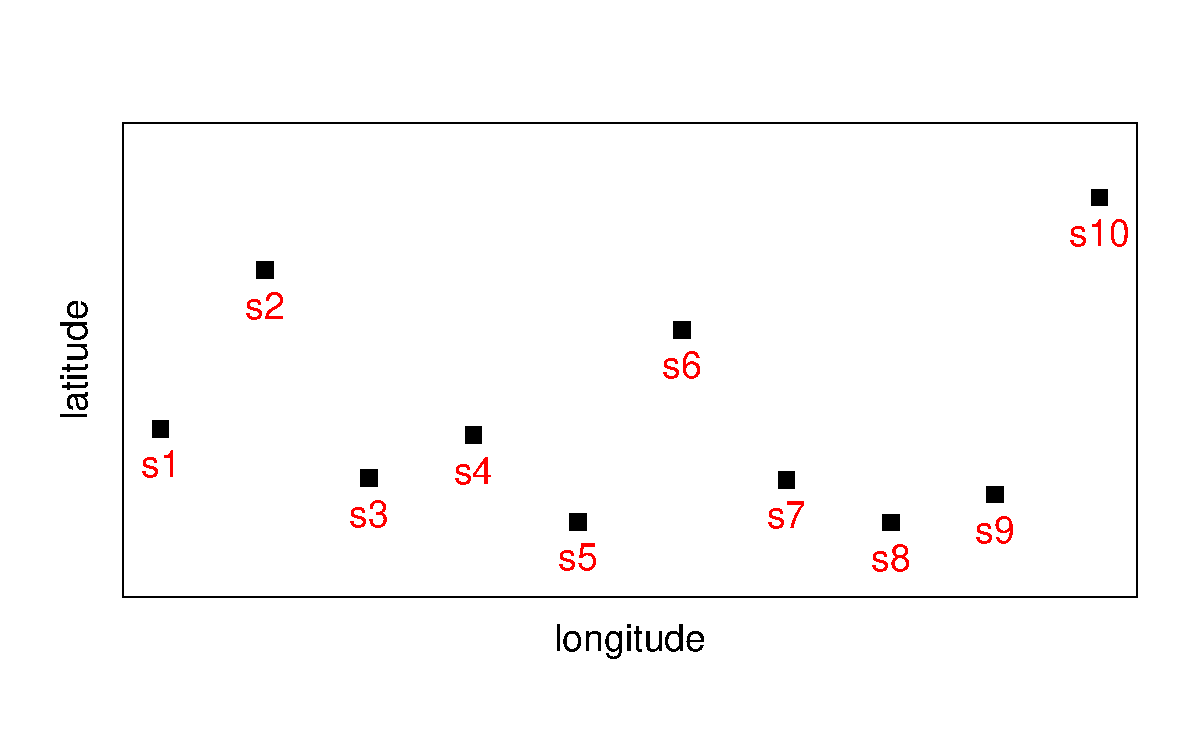
\includegraphics [width=0.8\textwidth, keepaspectratio]{graphs/location.pdf}
% \caption{Some arbitary saptial data at 10 random locations}
% \end{figure}


%\subsection{MSU data}

Since 1978 Microwave Sounding Units (MSU) measure radiation emitted by the earth's atmosphere from NOAA polar orbiting satellites. The different channels of the MSU measure different frequencies of radiation proportional to the temperature of broad vertical layers of the atmosphere. Tropospheric and lower stratospheric temperature data are collected by NOAA's TIROS-N polar-orbiting satellites and adjusted for time-dependent biases by the Global Hydrology and Climate Center at the University of Alabama in Huntsville (UAH)\footnote{\url{https://www.ncdc.noaa.gov/temp-and-precip/msu/overview}}. More information about how the data is been processed can be found in \cite{ChristySpencerBraswell2000}. Satellites do not measure temperature directly but measure radiances in various wavelength bands and then mathematically inverted to obtain the actual temperature.

% Channel 2 mainly measures tropospheric temperatures, while Channel 4 measures temperatures in the lower stratosphere. The analysis of the satellite temperature record represented here begins in 1979.

%%%%%%%%%%%%%%%%%%%%%%%%%%%%%%%%%%%%%%%%%%%%%%%%%%%%%%%%%%%%%%%%%%%%%%%%%%%%%%%%%%%%%%%%%%%%%%%%
\begin{figure}[H]
\label{MSU_data}
\centering
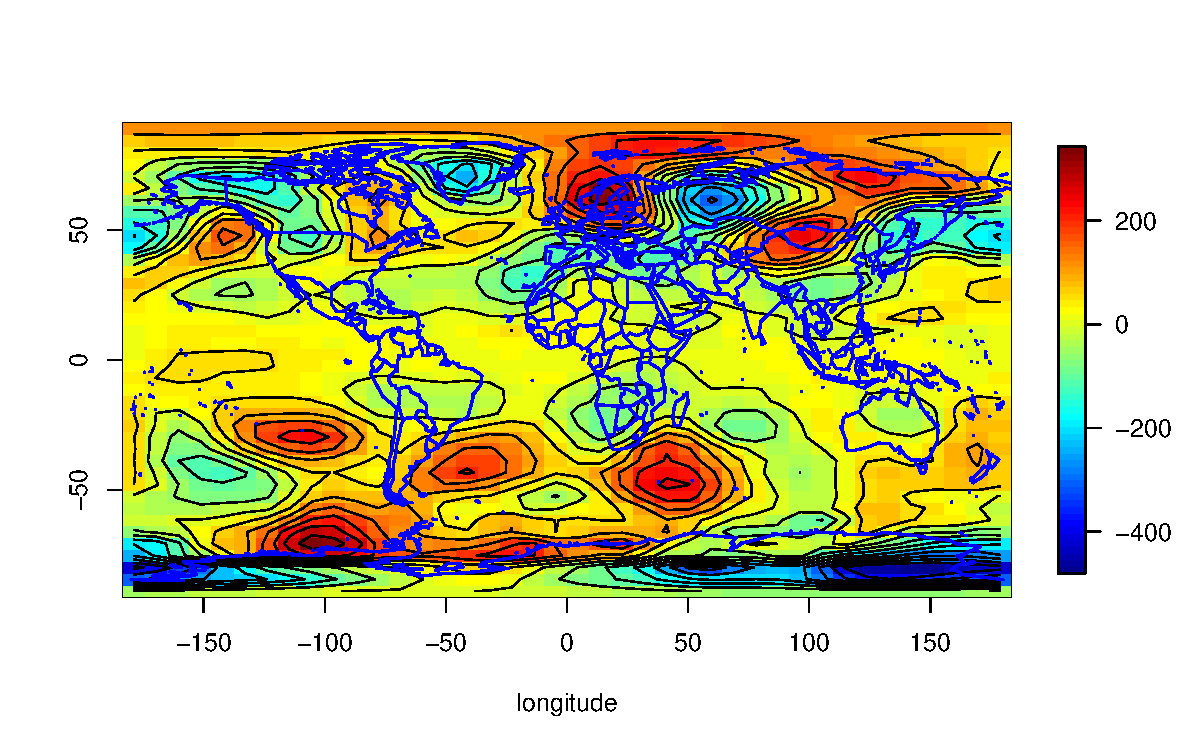
\includegraphics [width=0.8\textwidth, keepaspectratio]{graphs/MSU_data.pdf}
\caption[The MSU data were observed in August 2002 at $2.5^\circ \mbox{latitude} \times 2.5^\circ \mbox{longitude}$]{The MSU data were observed in August 2002 at $2.5^\circ \mbox{latitude} \times 2.5^\circ \mbox{longitude}$ with 10368 total number of observations.}
\end{figure}

\vfill



%%%%%%%%%%%%%%%%% below graph is not required
 % \begin{figure}[H]
 % \label{MSU_data_contour}
 % \centering
 % 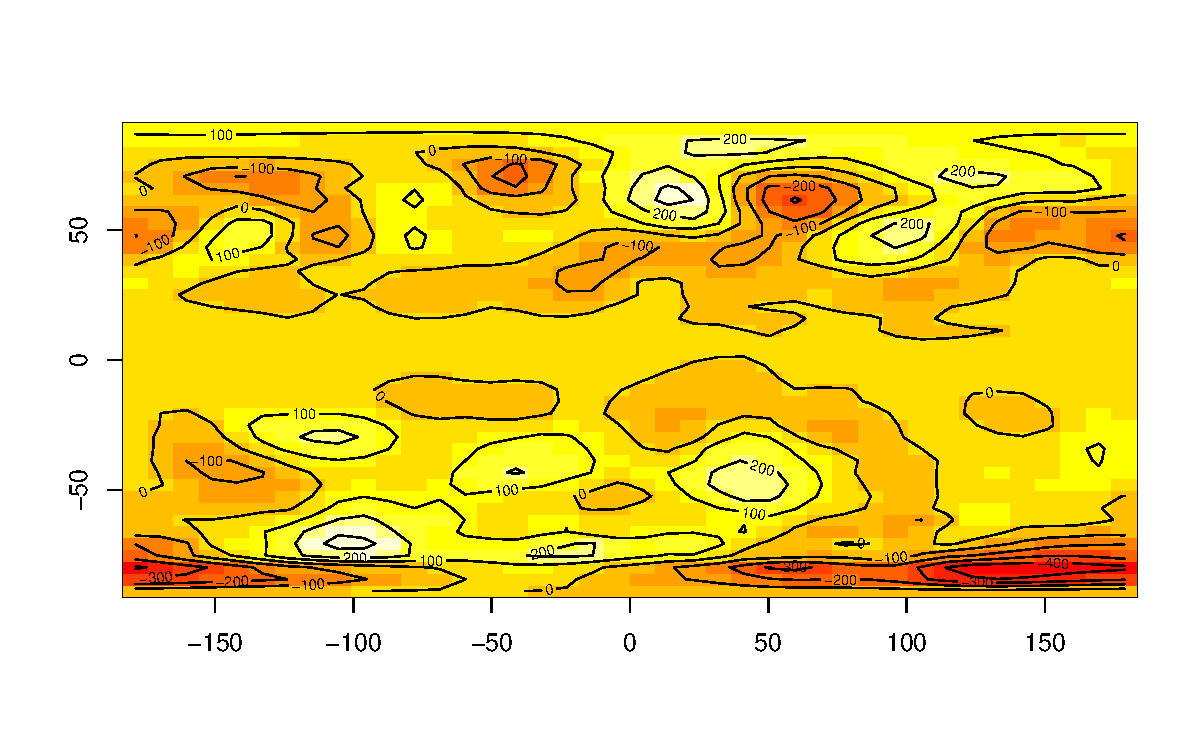
\includegraphics [height=4in, keepaspectratio]{MSU_data_contour.pdf}
 % \caption{August 2002, MSU data contour plot : resolution $2.5^0 latitude \times 2.5^0 longitude$}
 % \end{figure}


%%%%%%%%%%%%%%%%%%%%%%%%%%%%%%%%%%%%%%%%%%%%%%%%%%%%%%%%%%%%%%%%%%%%%%%%%%%%%%%%
\begin{figure}[H]
	\begin{subfigure}{.5\textwidth}
		\centering
		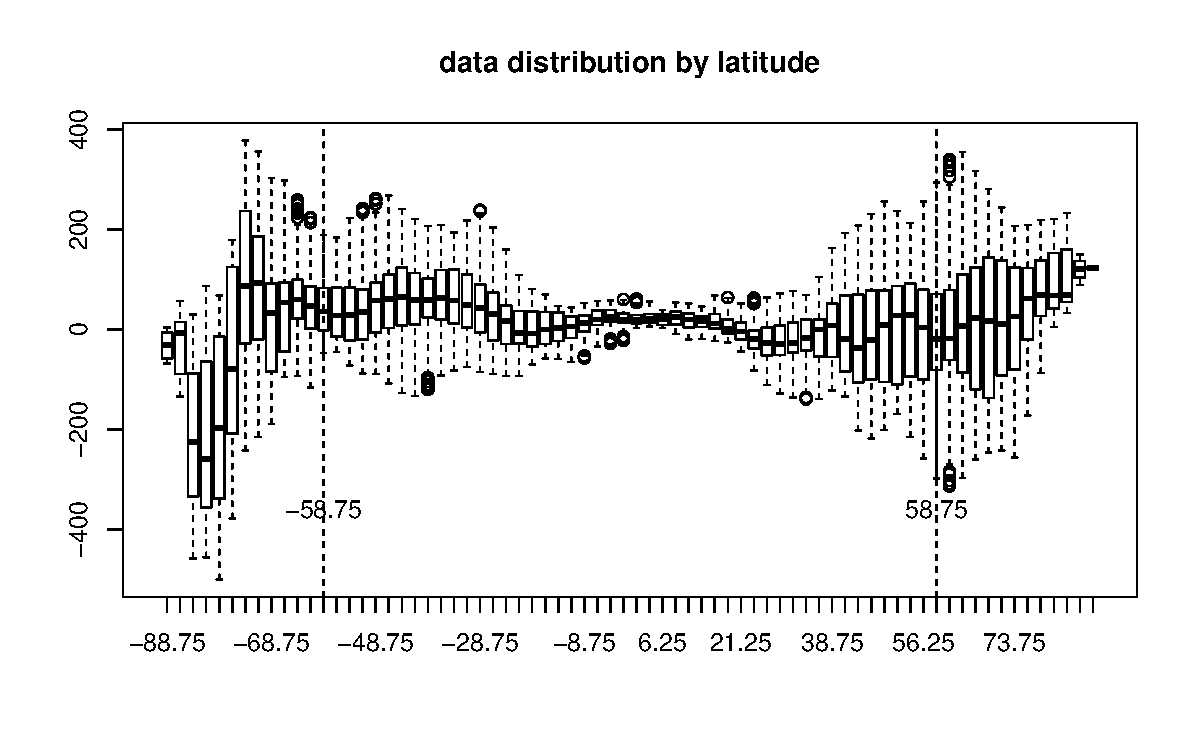
\includegraphics[width=1\linewidth]{graphs//MSU_data_latitude}
		\caption{distribution at each latitude}
		\label{MSU_data_latitude}
	\end{subfigure}
	\begin{subfigure}{.5\textwidth}
		\centering
		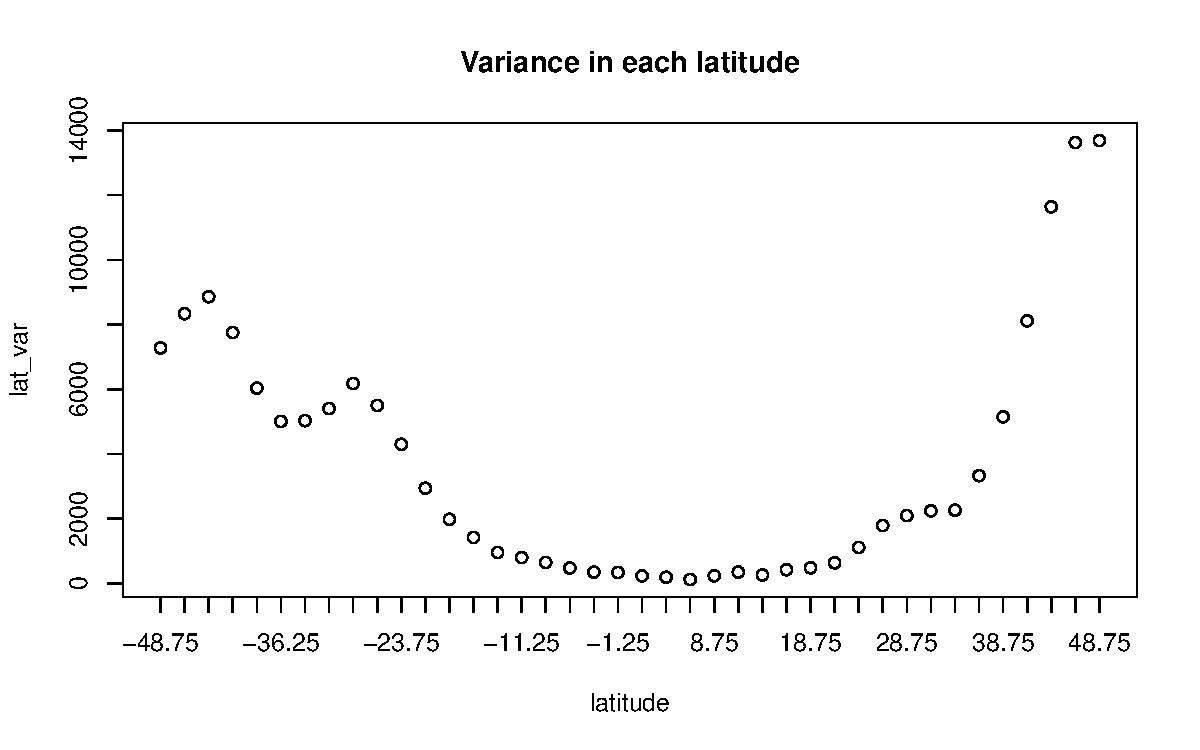
\includegraphics[width=1\linewidth]{graphs/MSU_data_var_lat}
		\caption{variance at each latitude}
		\label{MSU_data_var_lat}
	\end{subfigure}
	\caption[MSU data distribution at each latitude (data between $60^\circ S$ and $60^\circ N$]{MSU data distribution at each latitude (data between $60^\circ S$ and $60^\circ N$ were considered)}
	\label{compare_varigram_sim_2}
\end{figure}


Level 3 Total Ozone Mapping Spectrometer (TOMS) data \footnote{\url{http://disc.sci.gsfc.nasa.gov/data/datapool/TOMS}} is another popluar global data set discussed literature which has more than 20000 sapatial points (gridded points) (\cite{Stein2007}, \cite{CressieJohannesson2008}, \cite{JunStein2008}). There were some missing values in this data set. \cite{Stein2007} used the average of 8 neighboring locations to replace the missing values. They used spherical harmonics with associated Legendre polynomials of up to 78 covariates to remove the spatial trends to study axially symmetry (discussed in chapter 4) of the global data.

\vfill

% Extracted from \cite{Stein2007} ``The Nimbus-7 satellite carried a Total Ozone Mapping Spectrometer (TOMS) instrument that measured total column ozone daily from November 1, 1978 to May 6, 1993. This satellite followed a Sun-synchronous polar orbit with an orbital frequency of 13.825 orbits a day (cycle time about 104 minutes). As the satellite orbited, a scanning mirror repeatedly scanned across a track about 3000 km wide, each track yielding 35 total column ozone measurements. This version of the data is known as Level 2 and is . "

%%%%%%%%%%%%%%%%%%%%%%%%%%%%%%%%%%%%%%%%%%%%%%%%%%%%%%%%%%%%%%%%%%%%%%%%%%%%%%%%%%%%%%%%%%%%%%%%%%%%%%%
\begin{figure}[H]
\label{TOMS_data}
\centering
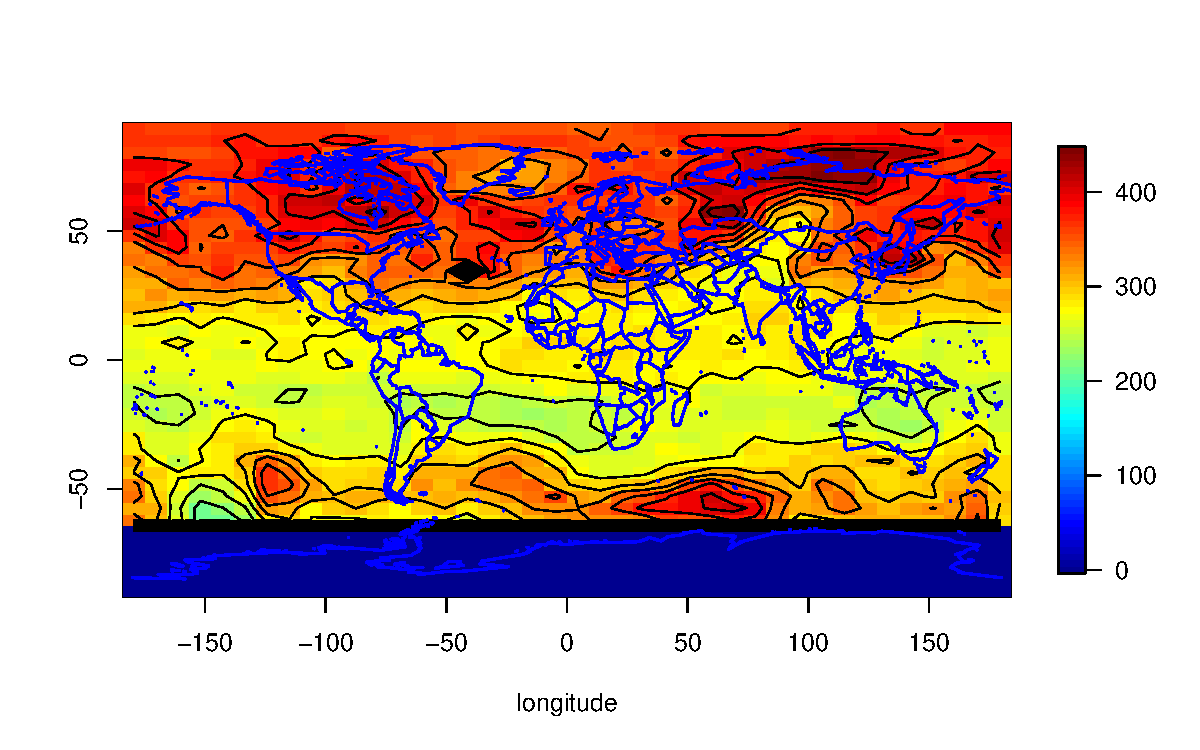
\includegraphics [width=0.8\textwidth, keepaspectratio]{graphs/TOMS_data.pdf}
\caption [TOMS data: resolution $1^\circ \mbox{latitude } \times 1.25^\circ \mbox{ longitude}$ in May, 1-6 1990.]{TOMS data: resolution $1^\circ \mbox{latitude } \times 1.25^\circ \mbox{ longitude}$ in May, 1-6 1990. The instrument used backscattered sunlight, therefore measurements were not available south of $73^\circ S$ during this week.}
\end{figure}

%%%%%%%%%%%%%%%%%%%%%%%%%%%%%%%%%%%%%%%%%%%%%%%%%%%%%%%%%%%%%%%%%%%%%%%%%%%%%%%%%%%%%%%%%%%%%%%%%%%%%%%%
\begin{figure}[H]
	\begin{subfigure}{.5\textwidth}
		\centering
		\includegraphics[width=1\linewidth]{graphs//TOMS_data_latitude}
		\caption{distribution at each latitude}
		\label{TOMS_data_latitude}
	\end{subfigure}
	\begin{subfigure}{.5\textwidth}
		\centering
		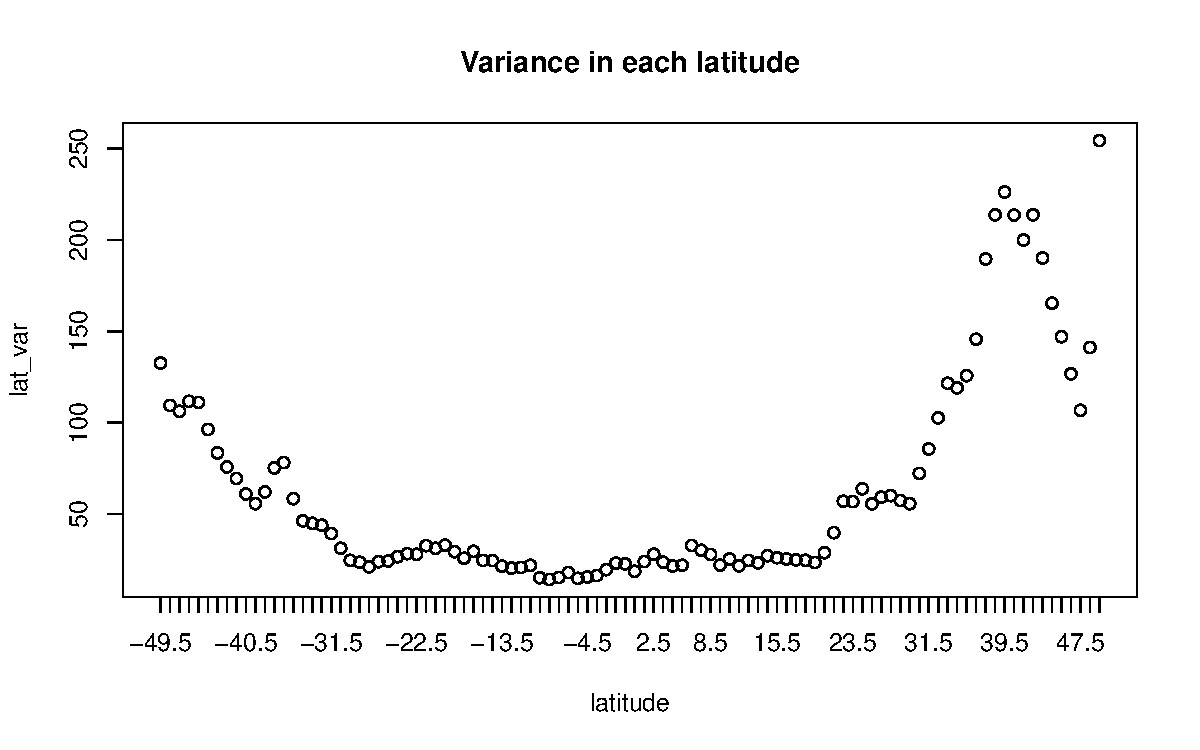
\includegraphics[width=1\linewidth]{graphs/TOMS_data_var_lat}
		\caption{variance at each latitude}
		\label{TOMS_data_var_lat}
	\end{subfigure}
	\caption[TOMS data distribution at each latitude (data between $50^\circ S$ and $50^\circ N$]{TOMS data distribution at each latitude (data between $50^\circ S$ and $50^\circ N$ were considered)}
	\label{compare_varigram_sim_2}
\end{figure}


Both MSU and TOMS data demonstrate strong variation when it is closer to Earth's poles. This shows the complexity of geospatial data. In addition, collecting geospatial data could be very expensive and time consuming. Next we discuss about the challenges when modeling spatial data.


 % \begin{figure}[H]
 % \centering
 % \includegraphics [width=0.8\textwidth, keepaspectratio]{graphs/TOMS_data_latitude.pdf}
 % \caption[OMS data: data distribution at each latitude (data between $50^\circ S$]{TOMS data: data distribution at each latitude (data between $50^\circ S$ and $50^\circ N$ were considered)}
 % \label{TOMS_data_latitude}
 % \end{figure}
 % 
 % \begin{figure}[H]
 % \centering
 % 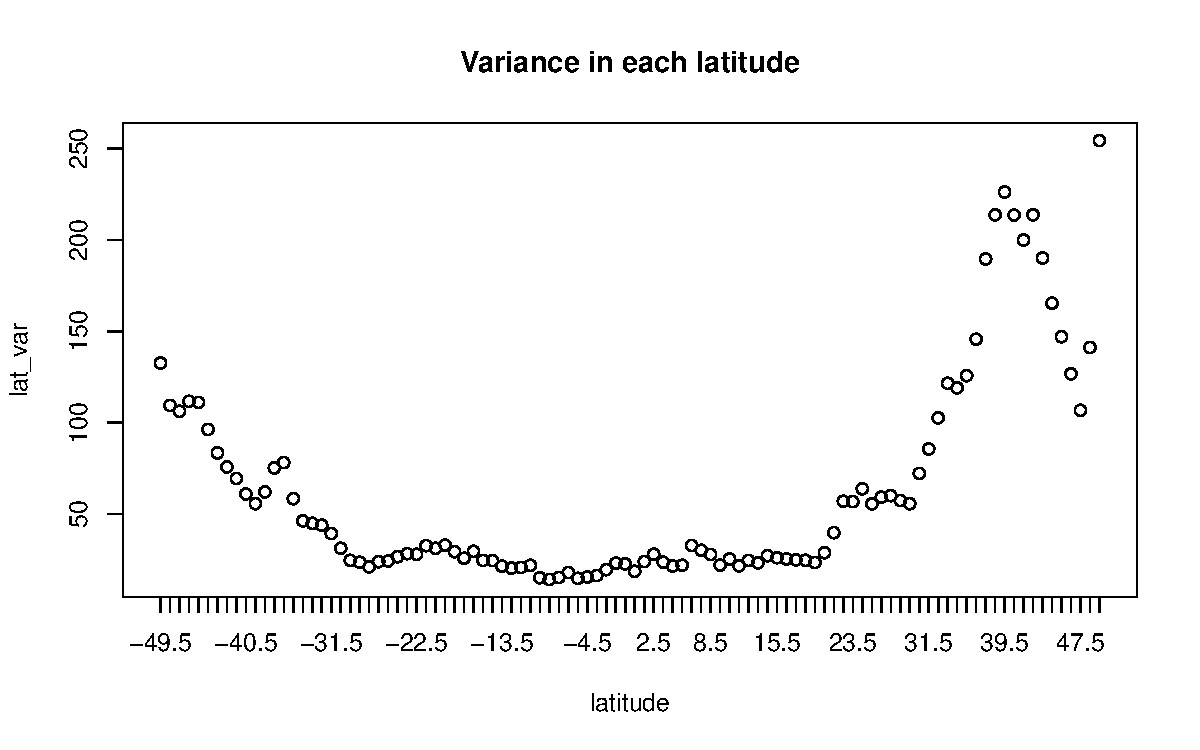
\includegraphics [width=0.8\textwidth, keepaspectratio]{graphs/TOMS_data_var_lat.pdf}
 % \caption{TOMS data: between $50^\circ S$ and $50^\circ N$, the variance at each latitude (variance is almost zero near the equator)}
 % \label{TOMS_data_var_lat}
 % \end{figure}

% \subsection{Challenges}



\section{Literature review}

There have been extensive statistical research on methodologies and techniques developed under the Euclidean space $R^d$. These approaches that are valid in $R^d$ have been applied to analyze global-scale data in recent years, due to global networks and satellite sensors that have been used to monitor a wide array of global-scale processes and variables. Here are some commonly used covariance models that are valid on $R^3$.

\begin{table}[H]
\label{parameters}
\centering
\begin{tabular}{|l|l|l|}
\hline
Family & C(h)  & Parameters \\ \hline \hline
$Mat\acute{e}rn$ &  $\frac{\sigma^2}{2^{\nu-1}\Gamma(\nu)} (\frac{h}{\phi})^{\nu} Y_{\nu}(\frac{h}{\phi})$  & $\nu, \sigma^2, \phi$  \\

Spherical & $\sigma^2(1-\frac{3h}{2\phi}+\frac{1}{2}(\frac{h}{\phi})^3)I_{0\le h\le \phi}$ & $\phi, \sigma^2$ \\

Exponential & $\sigma^2exp\{-(h/\phi)\}$ & $\phi, \sigma^2$  \\

Gaussian & $\sigma^2exp \{-(h/\phi)^2\}$ & $\phi, \sigma^2$  \\ \hline
%Power* & $\sigma^2(C_0-(h/\phi)^{\alpha}$ & $\phi, \sigma^2$ \\ \hline
\end{tabular}
\caption[Commonly used covariance models in $\R^3$]{Commonly used covariance models in $\R^3$} %* valid if $\alpha\in [0,2]$ }
\end{table}

However, this can have unforeseen impacts, such as making use of models that are valid in $R^d$ but in fact might not be valid under spherical coordinate systems. \cite{HuangZhangRobeson2011} have investigated some of commonly used covariance models that are valid in $R^d$, and they pointed out that many of those are actually invalid on the sphere. In particular they indicated (later proved by \cite{Gneiting2013}) that the commonly used $Mat\acute{e}rn$ covariance model is not valid if the smoothness parameter ($\nu$) is greater than 0.5, when modeling the homogeneous processes on the Earth. \\


%%%%%%%%%%%%%%% Discussion

The main emphasis of this dissertation is on random processes on a unit sphere. In particular, we focus on covariance models and estimation in modeling the global data. Note that the assumption of homogeneity on the sphere requires that the mean of the random process is constant and the covariance function of the process at two locations depends only on the spherical distance. This assumption is difficult to evaluate and often deemed unrealistic in practice. Several approaches on modeling non-homogeneity have been proposed in literature. For example, \cite{Stein2007} argued that Total Ozone Mapping Spectrometer (TOMS) data varies strongly with latitudes and homogeneous models are not suitable. Monte Carlo Markov Chain (MCMC) is another approach to model non-stationary covariance models on a sphere. \cite{Lindgren2011} analyzed global temperature data with a non-stationary model defined on a sphere using Gaussian Markov Random Fields (GMRF) and Stochastic Partial Differential Equations (SPDE). Further \cite{BolinLindgren2011} constructed a class of stochastic field models using SPDEs and non stationary covariance models were obtained by spatially varying the parameters in the SPDEs, where they claim that the method is more efficient than standard MCMC procedures. Furthermore, aerosol depth (AOD) from Multi-angle Imaging Spectrometer (MISR), Sea Surface Temperature (SST) from RRMM Microwave Imager (TMI) are some other examples for anisotropy global data on a sphere. \\

The analysis and modeling of axially symmetric data on the sphere has received increasing attention in literature in recent years. It was first introduced in \cite{Jones1963}, where the covariance of random processes between two spatial points depends on the longitudes only through their difference between those points. This assumption is more plausible and reasonable when modeling spatial data. For example, geophysical processes or variables such as temperature, moisture often exist homogeneity on longitudes rather than latitudes. \cite{Stein2007} used spherical harmonics to model (TOMS) data that exhibit an axial symmetry. \cite{JunStein2008} applied first-order differential operators to an isotropic process to draw conclusions about the local properties of axially symmetric spatio-temporal processes. \cite{HitczenkoStein2012} investigates the properties and theory of different forms of axially symmetric processes on the sphere.  \cite{Li2013} used convolution methods with $Mat\acute{e}rn$-type kernel functions to capture the non-stationarity of random fields on a sphere. \cite{Huang2012} developed a new and simplified representation for a valid axially symmetric process as well as explored the construction of parametric models for axially symmetric processes. \\

The computational cost for modeling and analyzing the axially symmetric data is very expensive. As we will see later in Chapter 4, the covariance function for axially symmetric processes requires triple summations, which one is to estimate $\mathcal{O}(n^3)$ parameters. Although the covariance structure given by \cite{Huang2012} might potentially reduce the number of parameters to be estimated in the order of $\mathcal{O}(n^2)$, the large data sets from global sensors and satellites often add much more computational cost. \cite{Stein2007} used 170 parameters from axially symmetric covariance structure to model TOMS data but was still not able to capture the global dependency. \cite{CressieJohannesson2008} used more than 396 parameters when they model the global data. Therefore, it is necessary to develop practically useful parametric models with easily interpretable parameters. \\

Statistical simulations have been one of the critical components in statistical research. Through simulations, the researcher can explore how a proposed statistical model/method behaves in the simulated and reproducible data that mimic the real applications. For axially symmetric processes, however, it seems in literature that there is lacking of the simulation method to generate global data that follow the axially symmetric covariance structure. Note that, as we will see later, the spectral representation of the process on the sphere is a summation of Legendre polynomials, which is distinct from its planar counterpart as represented by an integration of Bessel functions in $R^d$. This distinction could be understood through group representation theory, which possibly lies on the compactness of a sphere. Therefore, the estimation methods proposed based on $R^d$ should be reexamined for validity. All these areas are the basis for an exciting new line of research we are currently pursuing.

%----------------------------------------------%
\section{The outline of this dissertation}
%----------------------------------------------%

In Chapter 3 we explore some of the properties of commonly used covariance and variogram estimators on the circle based on Method of Moments (MOM). In contrast to the results given in time series and the Euclidean space, the MOM covariance estimator is biased and the true covariance function might not be identifiable based on the MOM estimator. On the other hand, the MOM variogram estimator is unbiased, but it is inconsistent. In Chapter 4 we first introduce the random process on the sphere. We then discuss the homogeneous process and the spectral representation for its covariance function on the sphere. Our main focus on this chapter is the axially symmetric process and its covariance function representation through the discrete fourier transform. The parametric models for characterizing such processes are also discussed. In particular, we extend the models given in \cite{Huang2012} and provide some graphical properties of those models. These generalized models will be fully implemented in Chapter 5 for axially symmetric data generation. In Chapter 5, we implement an algorithm to generate axially symmetric data based on the given covariance structure. We validate our generated data via simulations. Finally, Chapter 6 gives a summary of this research and provides further research directions.



%
%
%
% Monte Carlo Markov Chain (MCMC) is another approach to model non-stationary covariance models on a sphere. \cite{BolinLindgren2011} (continuation of the work proposed in \cite{Lindgren2011} ) constructed a class of stochastic field models using Stochastic Partial Differential Equations (SPDEs). Non stationary covariance models were obtained by spatially varying the parameters in the SPDEs, they argue that this method is more efficient than standard MCMC procedures.
%
% \cite{HitczenkoStein2012} discuss about the properties of an existing class of models for axially symmetric Gaussian processes on the sphere. They applied first-order differential operators to an isotropic process. draw conclusions about the local properties of the processes. Under some restrictions they derived explicit forms for the spherical harmonic representation of these processes covariance functions, and make conclusions about the local properties of the processes.
%
% $Mat\acute{e}rn$ covariance models are widely used when modeling spatial data, but when the smoothness parameter ($\nu$) is greater than 0.5 it is not valid for the homogeneous processes on the Earth surface with great circle distance. \cite{JeongJun2015} proposed $Mat\acute{e}rn$-like covariance functions for smooth processes on the earth surface that are valid with great circle distance (models were tested on sea levels pressure data).
%
% \begin{enumerate}
%
% \item Axially symmetry, which means that a process is invariant to rotations about the Earth's axis. The idea was first proposed by \cite{Jones1963}, where the covariance function depends on the longitudes only through their difference.
%
% \item In the study of a random process on a sphere, homogeneity (covariance depends solely on distance between locations) was assumed. However, this assumption may not be reasonable for actual data. \cite{Stein2007} argued that Total Ozone Mapping Spectrometer (TOMS) data varies strongly with latitudes and homogeneous models are not suitable. Further, \cite{CressieJohannesson2008}, \cite{JunStein2008}, \cite{BolinLindgren2011} pointed out that homogeneity assumption is not reasonable.
%
% \item There are no methods to test axially symmetry in real data. However, this assumption is more plausible and reasonable when modeling spatial data. For example, temperature, moisture, etc. most likely symmetric on longitudes rather than latitudes. \cite{Stein2007} propose a method to model axially symmetric process on a sphere (the fitted model is not the best, but this was a good start).
%
% \item There are no practically useful parametric models available, for our knowledge only models available so far, \cite{stein1999} with 170 parameters to estimate and \cite{CressieJohannesson2008} more than 396 parameters to estimate.
% %\blue{add description about the data}
%
% \item When modeling spatial data stationary models are less useful;\cite{JunStein2008} has proposed flexible class of parametric covariance models to capture the non-stationarity of global data. They used Discrete Fourier Transform (DFT) to the data on regular grids and calculated the exact likelihood for large data sets. Furthermore, they used Legendre polynomials to remove the spatial trends when fitting models to global data.
%
% \item \cite{Lindgren2011} analyzed global temperature data with a non-stationary model defined on a sphere using Gaussian Markov Random Fields (GMRF) and Stochastic Partial Differential Equations (SPDE)
%
% \item Monte Carlo Markov Chain (MCMC) is another approach to model non-stationary covariance models on a sphere. \cite{BolinLindgren2011} (continuation of the work proposed in \cite{Lindgren2011} ) constructed a class of stochastic field models using Stochastic Partial Differential Equations (SPDEs). Non stationary covariance models were obtained by spatially varying the parameters in the SPDEs, they argue that this method is more efficient than standard MCMC procedures. There are many articles followed this techniques but we will not discuss more details about these methods.
%
% \item Spatio-temporal mixed-effects model for dimension reduction was proposed by \cite{KatzfussCressie2011}. They used MOM parameter estimation method (similar approach in FRS). This work is also based on \cite{CressieJohannesson2008} spatial only Fixed Rank model. These methods are eventually focused on Bayesian approach and are less interested about topic.
%
% \item The previous studies have argued that many processes on a sphere are not homogeneous, especially in latitude direction. \cite{Huang2012} proposed a class of statistical processes that are axially symmetric and covariance functions that depend on longitudinal differences. Moreover, they have proposed longitudinally reversible processes and some motivations to construct axially symmetric processes. The covariance models implemented in this dissertation are modified versions of the covariance models proposed by \cite{Huang2012}.
%
% \item \cite{HitczenkoStein2012} discuss about the properties of an existing class of models for axially symmetric Gaussian processes on the sphere. They applied first-order differential operators to an isotropic process. draw conclusions about the local properties of the processes. Under some restrictions they derived explicit forms for the spherical harmonic representation of these processes covariance functions, and make conclusions about the local properties of the processes.
%
% %\item The issues associated when modeling axially symmetric spatial random fields on a sphere was discussed by \cite{Li2013}. They proposed convolution methods to generate random fields with a class of $Mat\acute{e}rn$-type kernel functions by allowing the parameters in the kernel function to vary with location. Moreover, they were able to generate flexible class of covariance functions and capture the non-stationary properties on a sphere. Used FFT to get the determinant and the inverse efficiently. Further, semi-parametric variogram estimation method using spectral representation was proposed for intrinsically stationary random fields on $S^2$.
%
% %\item \cite{HeatonKatzfussBerrettEtAl2014}
%
% \item  $Mat\acute{e}rn$ covariance models are widely used when modeling spatial data, but when the smoothness parameter ($\nu$) is greater than 0.5 it is not valid for the homogeneous processes on the Earth surface with great circle distance. \cite{JeongJun2015} proposed $Mat\acute{e}rn$-like covariance functions for smooth processes on the earth surface that are valid with great circle distance (models were tested on sea levels pressure data).
%
% \end{enumerate}


%\blue{Fill the above table later  }

%\end{document} 


%%------------------------------------------------------------------%%
\chapter{Asymptotics of estimators on a circle}
%\documentclass[12pt, amstex, letterpaper] {report} %{article}


\usepackage[margin=1in]{geometry}
\topmargin -0.5in \textwidth 6.5in \textheight 9in
\footskip .5in
\headheight 0.3in


\usepackage{Sweave}

\DefineVerbatimEnvironment{Sinput}{Verbatim} {xleftmargin=0em,frame=single}
\DefineVerbatimEnvironment{Soutput}{Verbatim} {xleftmargin=0em,frame=single}

\usepackage{amssymb, mathrsfs, amsmath, amsfonts}
\usepackage{enumerate, comment}
\usepackage{hyperref, natbib,apalike, float} %cite
\usepackage{color, multirow, setspace, fancyhdr,graphicx}
\usepackage{undertilde}
\usepackage[bottom]{footmisc}
\usepackage{graphicx}
\usepackage{framed}
\usepackage{subcaption}
\usepackage{amsthm}

%\doublespacing
\pagestyle{empty}
\pagestyle{fancy}
\lhead{ }
%\rhead{May 2016}
\fancyfoot{ }
\rfoot{Dissertation $|$ \thepage}
\lfoot{Chris Vanlangenberg}
\date{}

\includecomment{comment}

\newtheorem{theorem}{Theorem}[section]
\newtheorem{defn}{Definition}[section]
\newtheorem{prop}{Proposition}
\newcommand{\pro}[1]{\begin{prop}{#1}\end{prop}}

%\newtheorem{proof}{proof}
\newtheorem{rmk}{Remark}
\newcommand{\rmark}[1]{\begin{rmk}{#1}\end{rmk}}

\numberwithin{equation}{section}
\renewcommand{\footrulewidth}{0.1pt}
\renewcommand{\headrulewidth}{0.1pt}


\newcommand{\eqn}[1]{\begin{equation}{#1}\end{equation}}

\newcommand{\beq}{\begin{equation}}
\newcommand{\eeq}{\end{equation}}
%\renewcommand\refname{Literature}
\newcommand{\blue}[1]{\textcolor{blue}{\emph{#1}}}
\newcommand{\red}[1]{\textcolor{red}{\emph{#1}}}
\newcommand{\twoc}[2]{{\textcolor{blue}{#1}} and {\textcolor{red}{#2}}}


\newcommand{\xn}{x_1,\ldots, x_n}
\newcommand{\Xn}{X_1,\ldots, X_n}
\newcommand\floor[1]{\lfloor{#1}\rfloor}
\newcommand\ceil[1]{\lceil{#1}\rceil}

\newcommand{\X}{\mathcal{X}}
\newcommand{\Sp}{\mathbb{S}}
\newcommand{\R}{\mathbb{R}}
\newcommand{\C}{\mathbb{C}}
\newcommand{\pd}{positive definite }



\newcommand{\code}[1]{{\small\texttt{#1}}}
\newcommand{\pkg}[1]{{\normalfont\textsf{#1}}}
\newcommand{\var}[1] {{\normalfont\textbf{#1}}}
\newcommand{\Cm}{$C_m(\phi_P, \phi_Q)\ $}

\newcommand{\jun}{\cite{JunStein2008}}
%%
%\begin{document}

%%------------------------------------------------------------------%%
\section{Introduction}
%%------------------------------------------------------------------%%

For a stationary time series process, the covariance and variogram functions have been commonly used in the literature. More specifically, let $X(t)$ be a stationary process with unknown constant mean $\mu$ and covariance function $C(h), h \ge 0$. Let $\gamma(h) = C(0) - C(h)$ be the variogram function. For simplicity, we assume $\{X(t_k), k = 1, 2, \ldots, n\}$ is a sequence of random variables observed on gridded locations $\{t_k = (k-1)\delta, k \ge 1\}$ in $\R^1$ with $\delta = t_k - t_{k-1} > 0$ be the fixed interval length. First, note that $\bar{X} = \frac{1}{n}\sum_{k=1}^n X(t_k)$ is an unbiased estimator of $\mu$, and further under certain ergodic conditions, for example, the covariance function converges to zero as the lag $h \to \infty$. Thus,
\[
var(\bar{X}) \to 0, \quad \quad \mbox{as $n \to \infty$,}
\]
implying the consistency of $\bar{X}$ when estimating $\mu$ (for example \citealp{Cressie1993}).  \\

The covariance and variogram function estimators based on the method of moments (MOM) are given by
\begin{eqnarray*}
\hat{C}(h) &=& \frac{1}{n-h}\sum_{j = 1}^{n-h}(X(t_j+h) - \bar{X})(X(t_j) - \bar{X}), \quad \quad h = 1, 2, \cdots, n-1.  \\
2\hat{\gamma}(h) &=& \frac{1}{n-h}\sum_{j = 1}^{n-h}(X(t_j+h) - X(t_j))^2, \quad \quad h = 1, 2, \cdots, n-1,
\end{eqnarray*}
respectively. It has been shown (for example \citealp{Cressie1993}) that both the variogram and covariance MOM estimators are biased. While the bias for the covariance MOM estimator is of the rate of $O(1/n)$, the bias for the variogram MOM estimator is smaller. Furthermore, the asymptotic joint Gaussianity of the estimators $\{\hat{C}(h)\}$ and $2\hat{\gamma}(h)$ has also been established under the same ergodic conditions ({\em i.e.}, conditions that ensure the dependence in the process dies off sufficiently quickly as the lag distance increases). Finally, for fixed $h$, both the variances and covariances of $\{\hat{C}(h)\}$ and of $2\hat{\gamma}(h)$ can be found (for example, in \citealp{fuller2009introduction, cressie1985fitting}) as of $O(1/n)$, which demonstrates the consistency of both estimators. Parallel results can also be obtained for the covariance and variogram MOM estimators in $\R^d$ \citep{Cressie1993}. \\

There are two distinct asymptotics in spatial statistics: increasing domain asymptotics, where more data are collected by increasing the domain, and fixed-domain or infill asymptotics, where more data are collected by sampling more densely in a fixed domain. Asymptotic properties of estimators are quite different under the two asymptotics. The above asymptotics in the time series and $\R^d$ belong to the first one. There have been extensive discussions of the infill asymptotics in the literature. For example, \cite{Zhang:2004:IEA} showed that for the popularly used Mat\'{e}rn covariance model, one cannot correctly distinguish between two Mat\'{e}rn covariances with probability one no matter how many sample data are observed in a fixed region. Consequently, not all covariance parameters in Mat\'{e}rn models are consistently estimable. However, discussion about the asymptotics on the circle and sphere is lacking. In particular, with the increasing interest in the study of global data on the sphere, it is necessary that the infill asymptotics of existing estimators be examined. As the first step for the study of the asymptotics of covariance and variogram estimators on the sphere, we consider their asymptotics on the circle. \\

This chapter is organized as follows. We first introduce the random processes on the circle and then give the spectral representation of the covariance and variogram functions for stationary processes. Under the assumption of stationary Gaussian process on the circle, we show that the unbiased estimator $\bar{X}$ is not consistent when estimating $\mu$. Then, we demonstrate that the covariance function estimator based on MOM is biased with non-estimable bias, while the variogram MOM estimator is unbiased but inconsistent. Our results are supplemented via simulations.

\vskip 8pt
%%------------------------------------------------------------------%%
\subsection{Random Process on a Circle}
%%------------------------------------------------------------------%%

Let $X(t)$ be the random process on the unit circle $\Sp^1$. If $X(t)$ is further assumed to be with finite second moment and continuity in quadratic mean, then $X(t)$ can be represented in a Fourier series which is convergent in quadratic mean \citep{DUFOUR1976107},
\[
X(t) = A_0 + \sum_{n=1}^\infty (A_n\cos(nt) + B_n \sin(nt)), \quad \quad t \in \Sp^1,
\]
where
\begin{eqnarray*}
A_0 = \frac{1}{2\pi}\int_S X(t)dt, \quad A_n = \frac{1}{\pi}\int_S X(t)\cos(nt)dt, \quad B_n = \frac{1}{\pi}\int_S X(t)\sin(nt)dt.
\end{eqnarray*}
Let $s, t \in \Sp^1$. The covariance function $C(s, t)$ of the process $X(t)$ on the given locations $s$ and $t$ is given below
\begin{eqnarray*}
C(s, t) = cov(X(s), X(t)).
\end{eqnarray*}
Now we assume the underlying process $X(t)$ is stationary on the circle, that is, $E(X(t)) = \mu$ unknown, and its covariance function solely depends on the angular distance $\theta$,
\[
C(\theta) = cov(X(t+\theta), X(t)), \quad \quad \theta \in [0, \pi].
\]
Under the assumption of stationarity, we have
\begin{eqnarray*}
cov(A_n, A_m) = cov(B_n, B_m) = a_n \delta(n, m), \quad \mbox{and} \quad cov(A_n, B_m) = 0, \quad \mbox{for $n \ge 0, m > 0$},
\end{eqnarray*}
with $a_n \ge 0$, and $\delta(n,m)=1$ if $n=m$, and 0 otherwise. Further the covariance function $C(\theta)$ can be written as the following spectral representation:
\begin{eqnarray*}
C(\theta) = a_0 + \sum_{n=1}^\infty a_n \cos(n\theta), \quad \quad \mbox{for $\theta \in [0, \pi]$}.
\end{eqnarray*}
By the orthogonality of $\{\cos(n\theta), n = 0, 1, 2, \cdots,\}$ on $\theta \in [0, \pi]$, we have
\[
a_0 = \frac{1}{\pi}\int_0^\pi C(\theta)d\theta, \quad \quad a_n = \frac{2}{\pi}\int_0^\pi C(\theta)\cos(n\theta)d\theta, \quad n \ge 1.
\]
If a random process $X(t)$ is intrinsically stationary, one has $E(X(t)) = \mu$, an unknown constant, and the variogram function depends only on the angular distance $\theta$, given by
\begin{eqnarray*}
\gamma(\theta) = var(X(t+\theta) - X(t)), \quad \quad t \in \Sp^1.
\end{eqnarray*}
Note that if $X(t)$ is stationary, then
\[
\gamma(\theta) = C(0) - C(\theta).
\]
Equivalently, $\gamma(\theta)$ has the following spectral representation
\[
\gamma(\theta) = \sum_{n = 1}^\infty a_n (1 - \cos(n\theta)).
\]


%-------------------------------------%
\subsection{Mean and Covariance Estimation on the Circle}
%-------------------------------------%

We now consider estimation of the unknown mean $\mu$ and covariance function $C(\theta)$. Let $\{X(t_k), k = 1, 2, \cdots, n\}$ be a collection of gridded observations on the unit circle, with $t_k = (k-1)*2\pi/n, k = 1, 2, \cdots, n$. For simplicity, let $n = 2N$ be an even number. Denote $\utilde{X} = (X(t_1), X(t_2), \cdots, X(t_n))^T$ as the observed random vector. When the underlying process $X(t)$ is stationary on the unit circle, the variance-covariance matrix of $\utilde{X}$ given by

\begin{eqnarray*}
	\Sigma &=& \left(\begin{array}{ccccccc}
	C(0)      & \cdots & C((N-1)\delta ) & C(\pi) &  C((N-1)\delta ) & \cdots & C(\delta) \\
	C(\delta) & \cdots & C((N-2)\delta) & C((N-1)\delta) &  C(\pi)  & \cdots & C(2\delta) \\
	C(2\delta) & \cdots & C((N-3)\delta) & C((N-2)\delta) &  C((N-1)\delta) & \cdots & C(3\delta)\\
	\vdots    & \vdots  & \vdots  & \vdots  & \vdots  & \vdots  & \vdots  \\
	C(\delta) & \cdots & C(\pi) &  C((N-1)\delta) & C((N-2)\delta)  & \cdots & C(0)
	\end{array} \right)
\end{eqnarray*}
where $\Sigma$ is a symmetric circulant matrix with elements
\[
C(0),C(\delta), C(2\delta), \cdots, C((N-1)\delta), C(\pi),  C((N-1)\delta), \cdots, C(\delta), \mbox{ where } \delta = 2\pi/n.
\]
Therefore the sample mean (denoting $\utilde{1}_n = (1,1,\dots,1)_{n\times 1}^{T}$), 
\[
\bar{X} = \frac{1}{n}\utilde{1}_n^T \utilde{X}
\]
is an unbiased estimator of $\mu$ with variance given by
\begin{eqnarray*}
var(\bar{X}) &=& cov\left(\frac{1}{n}\utilde{1}_n^T \utilde{X}, \frac{1}{n}\utilde{1}_n^T \utilde{X}\right) \nonumber \\
	&=& \frac{1}{n^2}\utilde{1}_n^T \Sigma \utilde{1}_n \nonumber \\
	&=& \frac{1}{n} \left(C(0)+C(\pi)+2 \sum_{m=1}^{N-1}C(m 2\pi/n)\right). \nonumber
\end{eqnarray*}

If we assume that $C(\theta)$ is a continuous function on $[0, \pi]$ and note the summation in the last quantity is a trapezoid sum of $C(\theta)$ on the gridded locations within $[0, \pi]$, then,
\[
\frac{1}{\pi} \frac{\pi}{2 N} \left(C(0) + \sum_{m=1}^{N-1}C(m 2\pi/n) + C(\pi) \right) \to \frac{1}{\pi} \int_0^\pi C(\theta)d\theta = a_0,
\]
as $n \to \infty$. That is, $var(\bar{X}) \to a_0$ as $n \to \infty$. Therefore, we have the following proposition.

\pro{ \label{prop3.1}
The sample mean $\bar{X}$ is an unbiased estimator of $\mu$ with the asymptotic variance of $a_0$. If $a_0 > 0$ and $X(t)$ is further assumed to be Gaussian, then $\bar{X}$ is NOT a consistent estimator of $\mu$.
}

\begin{proof}
It is only necessary to prove the second part. If $X(t)$ is Gaussian, then $\bar{X} \sim N(\mu, var(\bar{X})) \Rightarrow Z = \frac{\bar{X} - \mu}{\sqrt{var(\bar{X})}} \sim N(0, 1)$. First, for a fixed $\varepsilon_0 > 0$ and $\varepsilon_0 < a_0$, there exists $K$, such that for all $n > K$, we have
\[
|var(\bar{X}) - a_0| < \varepsilon_0 \Rightarrow a_0 - \varepsilon_0 < var(\bar{X}) < a_0 + \varepsilon_0.
\]
Now for each fixed $\varepsilon > 0$ and all $n > K$,
\begin{eqnarray*}
P\left(|\bar{X} - \mu| > \varepsilon\right) &=& P\left(\frac{|\bar{X} - \mu|}{\sqrt{var(\bar{X})}} > \frac{\varepsilon}{\sqrt{var(\bar{X})}} \right) \\
&\ge& P\left(|Z| > \frac{\varepsilon}{\sqrt{a_0 - \varepsilon_0}} \right) > 0.
\end{eqnarray*}
Hence $\bar{X} \not\to \mu$ in probability. The last inequality above is due to the following.
\[
\left\{|Z| > \frac{\varepsilon}{\sqrt{a_0 - \varepsilon_0}} \right\} \subseteq \left\{|Z| > \frac{\varepsilon}{\sqrt{var(\bar{X})}}\right\}.
\]

\end{proof}


\vskip 8pt

\rmark{Under the assumption of Gaussianity, Proposition \ref{prop3.1} indicates that $\bar{X}$ will never be a consistent estimator for $\mu$, which contrasts to the result given in time series and $\R^d$.}

\vskip 8pt

\rmark{\label{remark2} Recall that, if $X(t)$ is a stationary process on the circle, we have
\[
a_0 = var(A_0)
\]
and $\mu = E(A_0)$. Therefore, $a_0 = 0 \Rightarrow \mu = 0$, under which $var(\bar{X}) \to 0$ and so $\bar{X}$ is consistent. In other words, if $a_0 = 0$ so that $X(t)$ is a zero mean stationary process on the circle, then $\bar{X}$ is an unbiased and consistent estimator of $\mu = 0$.}

\vskip 8pt

\rmark{If in practice, we have multiple copies of data observations on the circle, we can then estimate $a_0$ or $var(\bar{X})$ through these copies. More explicitly, suppose that we have {\em i.i.d.} copies of the random samples on the circle with averages denoted as $\{\bar{X}_i, i = 1, 2, \cdots, m\}$. We then use the method of moments to estimate $a_0$, which is given as following:
\[
\hat{a}_0 = \frac{1}{m-1} \sum_{j=1}^m (\bar{X}_j - \bar{\bar{X}})^2,
\]
where $\bar{\bar{X}} = \frac{1}{m} \sum_{k = 1}^m \bar{X}_k$. Under some regularity conditions, one can show that $\hat{a}_0$ is an unbiased and consistent estimator of $a_0$.}

\vskip 16pt

%-------------------------------------%
\section{Data Generation on a Circle}
%-------------------------------------%

To explore the properties of the MOM estimator, we performed a simulation study. We consider two covariance functions that are valid on a circle; exponential and power families as given below:
\begin{eqnarray}
\label{exp_cov}
C(\theta) &=& C_1e^{-a|\theta|} \quad a>0, C_1>0, \theta \in [0, \pi], \\
\label{power_cov}
C(\theta) &=& c_0 - (|\theta|/a)^{\alpha} \quad a>0, \alpha \in (0,2].
\end{eqnarray}
where $\theta \in [0,\pi]$ and  $c_0 > 0$ satisfies $c_0 \ge \int_0^\pi(\theta/a)^{\alpha} \sin \theta d \theta$. \\

%\begin{figure}
%	\centering
%	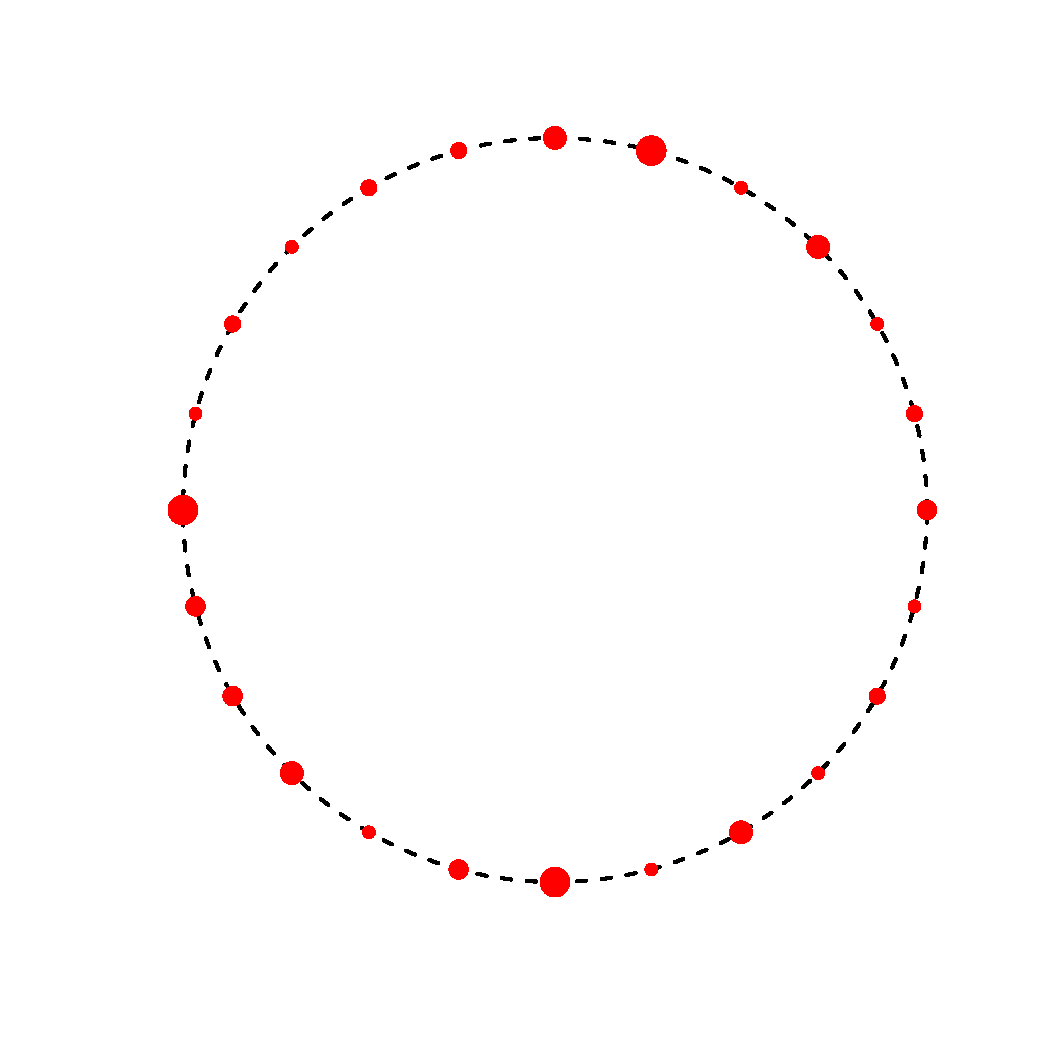
\includegraphics[width=0.5\textwidth]{graphs/process_circle}
%	\caption {Random process on a circle at 24 points ($\Delta\lambda = 15^0$), the red dots represent the  observed values at a given time and each point is associated with a random process of its own.}
%\end{figure}

Recall that $\utilde{X} = (X(t_1), X(t_2), \ldots, X(t_n))^T$ is the observed gridded data on the circle. Its variance-covariance matrix $\Sigma$ is symmetric and circulant. Hence it can be 
decomposed as
\[
\Sigma = Q \Lambda Q^T,
\]
where $\Lambda=\mbox{diag}\{\lambda_1, \lambda_2,\cdots,\lambda_n\}$ and $Q=\{\psi_1, \psi_2,\cdots,\psi_n\}$ with $\lambda_i, i = 1, 2 \ldots, n$, are eigenvalues and $\psi_1, \psi_2,\cdots,\psi_n$ are eigenvectors of the circulant matrix, respectively. (See Section 1.3). Therefore, let $\utilde{Z}$ be {\em i.i.d.} standard normal random variates. Then
\[
	\utilde{X} = \Sigma^{1/2}*\utilde{Z} = Q\Lambda^{1/2}Q^T*\utilde{Z},
\]
is the observed data vector that follows the given covariance function.

\vskip 16pt

%-------------------------------------%
\section{Covariance MOM Estimator}
%-------------------------------------%

Now we consider the MOM estimator of $C(\theta)$, which is given by
\beq \label{covarince_estimator}
\hat{C}(\Delta \lambda) = \frac{1}{n}\sum_{i = 1}^n (X(t_i + \Delta \lambda) - \bar{X})(X(t_i) - \bar{X}),
\eeq
where $\Delta \lambda = 0, 2\pi/n, 4\pi/n, \cdots, 2(N-1)\pi/n$ (for simplicity, we set $n=2N$ even). \\

For the simulation, we set $C_1 = a = 1$ and choose $\alpha = 0.5$, $c_0 \ge \int_0^\pi(\theta)^{0.5} \sin(\theta) d\theta$. From the Fresnel integral, it can be shown that $c_0 \ge 2.4353$. Now we compare the covariance estimator (empirical) to its theoretical covariance given by \eqref{exp_cov} and \eqref{power_cov}, respectively. We computed the MOM estimator $\hat{C}(\theta)$ with $n = 48$ gridded observations on the circle with 500 repetitions.

      \begin{figure}
      	\centering
       	% 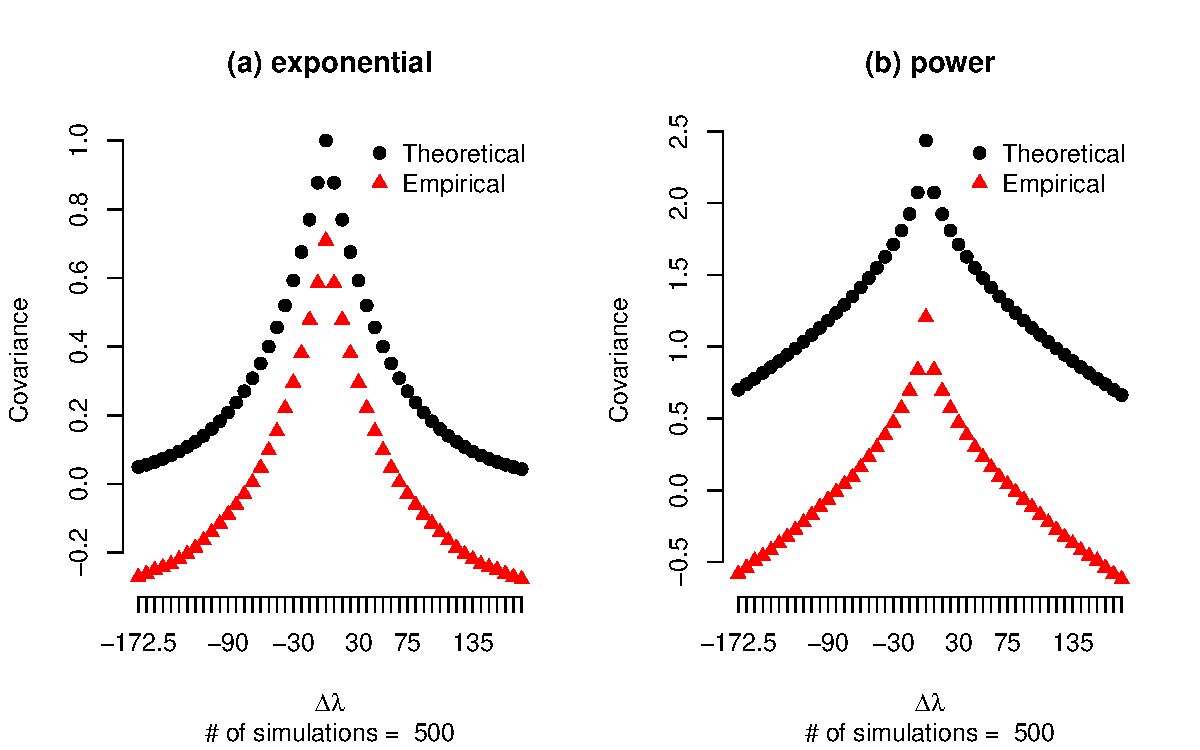
\includegraphics[width=0.9\textwidth]{graphs/covarince_circle}
       	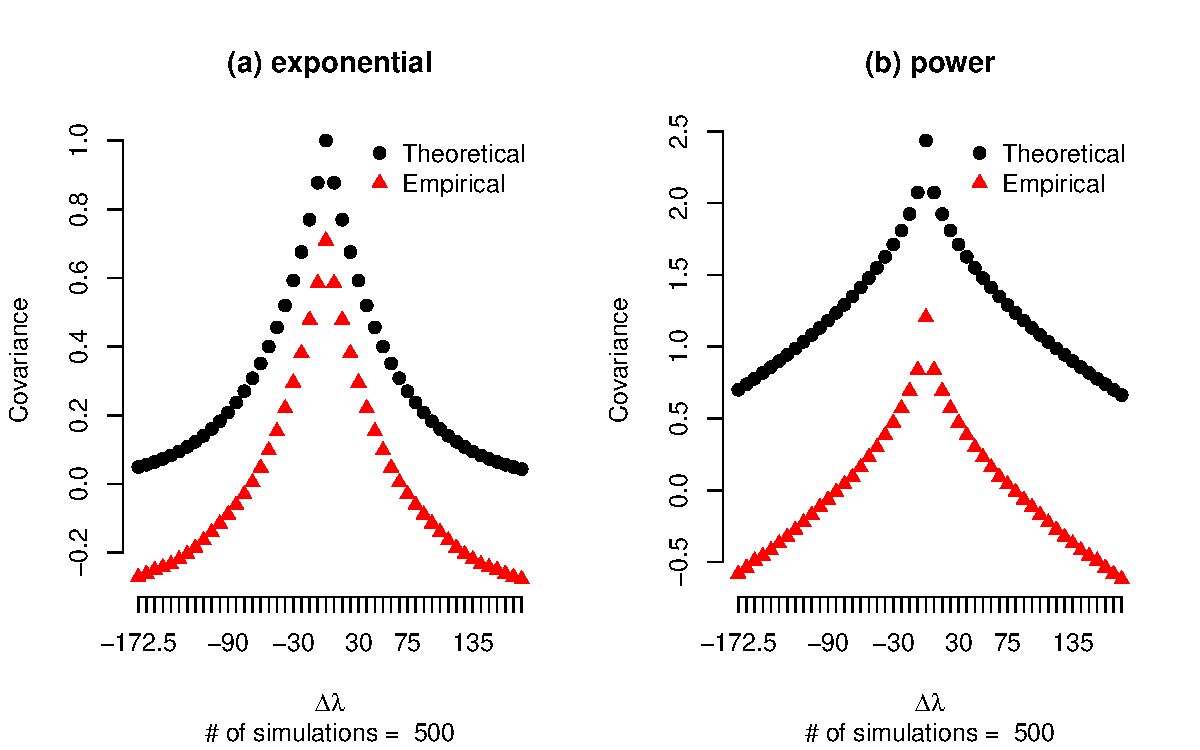
\includegraphics[keepaspectratio, scale = .8]{graphs/covariance_circle.pdf}
      	\caption[Comparison Between Theoretical and Empirical Covariances Without] {Comparison between theoretical and empirical covariances without any adjustments on a circle. }
      	\label{covariance_circle}
      \end{figure}
      
\rmark{One can easily notice a shift between the theoretical and empirical values appearing on both graphs (Figure \ref{covariance_circle}). The shift  can be shown to be approximately equal to $a_0$, where $a_0 = \frac{1}{\pi}\int_0^\pi C(\theta)d\theta$. For both covariance functions considered, we can obtain	
\begin{eqnarray*}
	    \mbox{exponential family: }  	a_0 &=& \frac{C_1}{a\pi}(1 - e^{-a\pi}), \\
	    \mbox{power family: }  	a_0       &=& c_0 - \left(\frac{\pi}{a}\right)^{\alpha}\frac{1}{\alpha + 1}.
\end{eqnarray*}
}
Next we consider the covariance function $D(\theta)$, after subtracting $a_0$ from $C(\theta)$. Since the bias seems to be equal to $a_0$
	      \[
	      	D(\theta) = C(\theta) - a_0.
	      \]
From Remark \ref{remark2}, $D(\theta)$ is now the covariance function of a stationary process on the circle. Where the constant term of its spectral representation equals to zero. The simulation setup is the same as above except that $C(\theta)$ is replaced with $D(\theta)$. The results show that the empirical and theoretical values match very well (Figure \ref{covariance_remove_a0}). 

\vskip 8pt

	      \begin{figure}
	      	\centering
	      	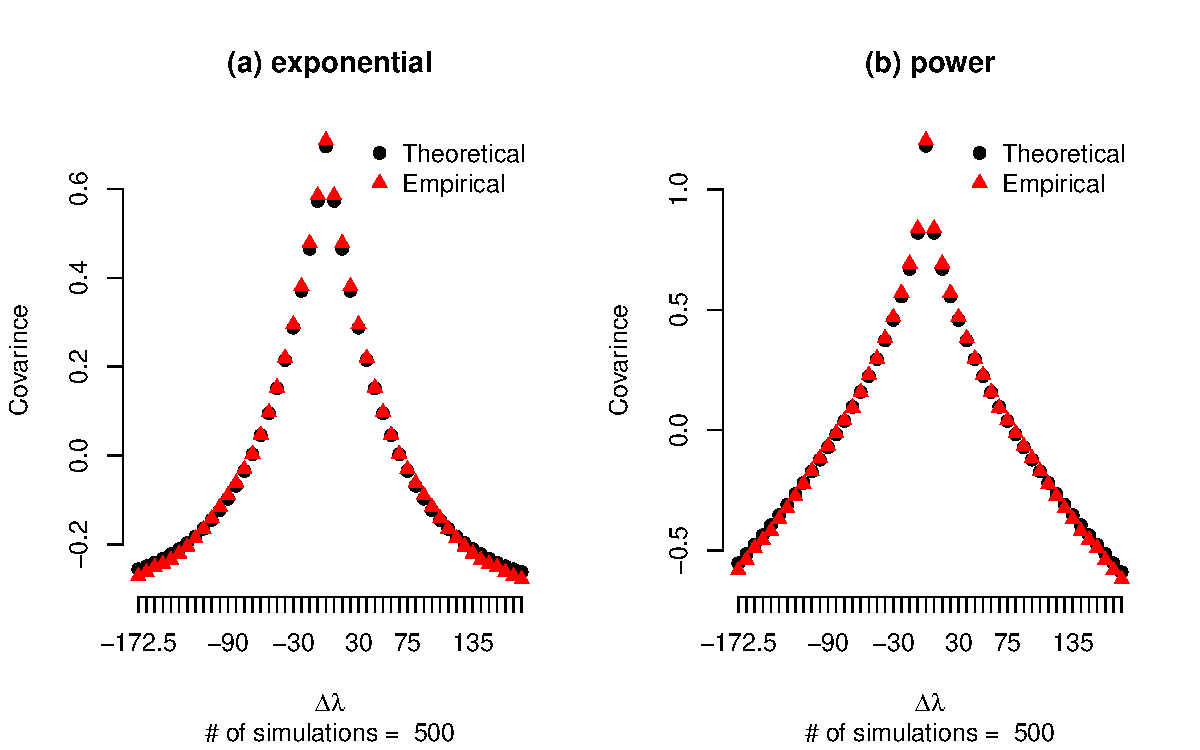
\includegraphics[width=0.8\textwidth]{graphs/covarince_circle_remove_a0}
	      	% 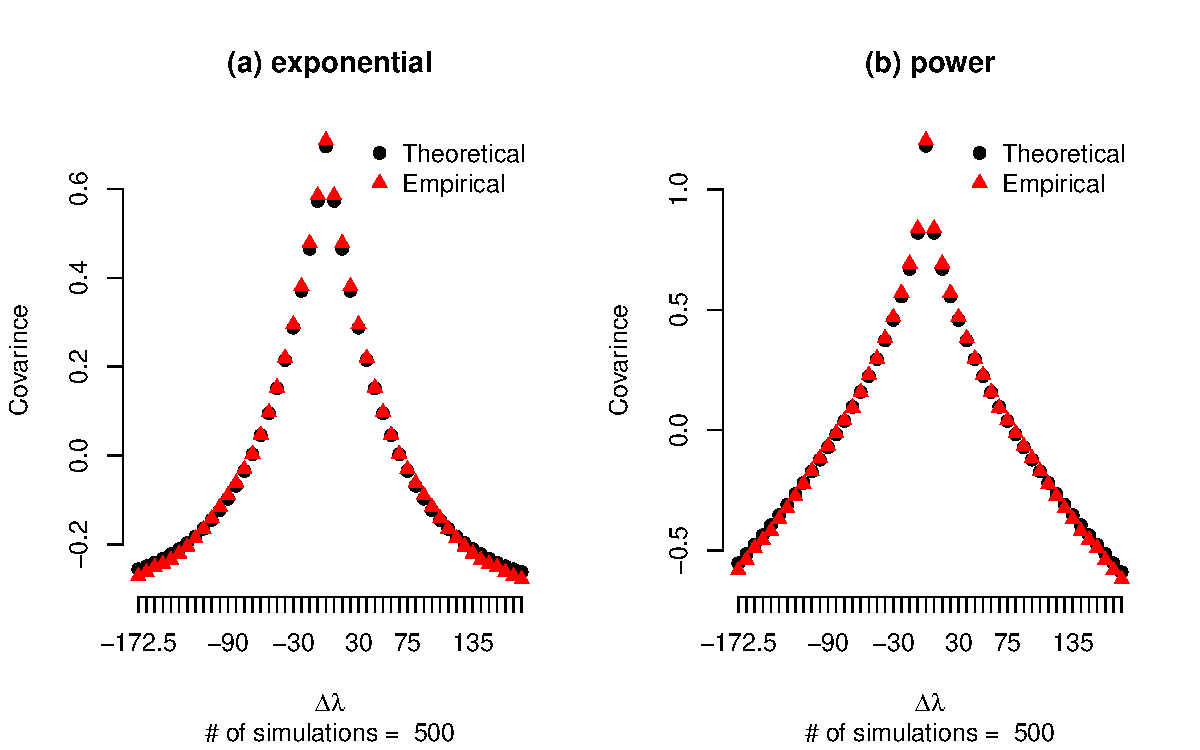
\includegraphics[scale=.8, keepaspectratio]{graphs/covarince_circle_remove_a0.pdf}
	      	%graph from data genaration summary doc line 194
	      	\caption[Theoretical and Empirical Covariance Comparison on a Circle Using The]{Theoretical and empirical covariance comparison on a circle using the modified covariance function $D(\theta)$.}
	      	\label{covariance_remove_a0}
	      \end{figure}

\rmark{ The covariance estimator is biased and the bias is close to $a_0$, which is non-estimable. However if {\em i.i.d.} copies of random data on the same circle are available then one can estimate $a_0$ {\em i.e.}, $\hat{a} = var(\bar{X})$. The new covariance estimator could then be estimated by subtracting $\hat{a}_0$ form the original MOM estimator as given below.
% \[
% \hat{C}(\Delta \lambda) = \left( \frac{1}{n}\sum_{i = 1}^n (X(t_i + \Delta \lambda) - \bar{X})(X(t_i) - \bar{X}) \right) -  \hat{a}_0.
% \]
\[
\tilde{C}(\Delta \lambda) = \hat{C}(\Delta \lambda) -  \hat{a}_0.
\]
}
Our simulation shows both curves match very well (Figure \ref{covariance_estimate_a0}).
	
	\begin{figure}[H]
	 \centering
	 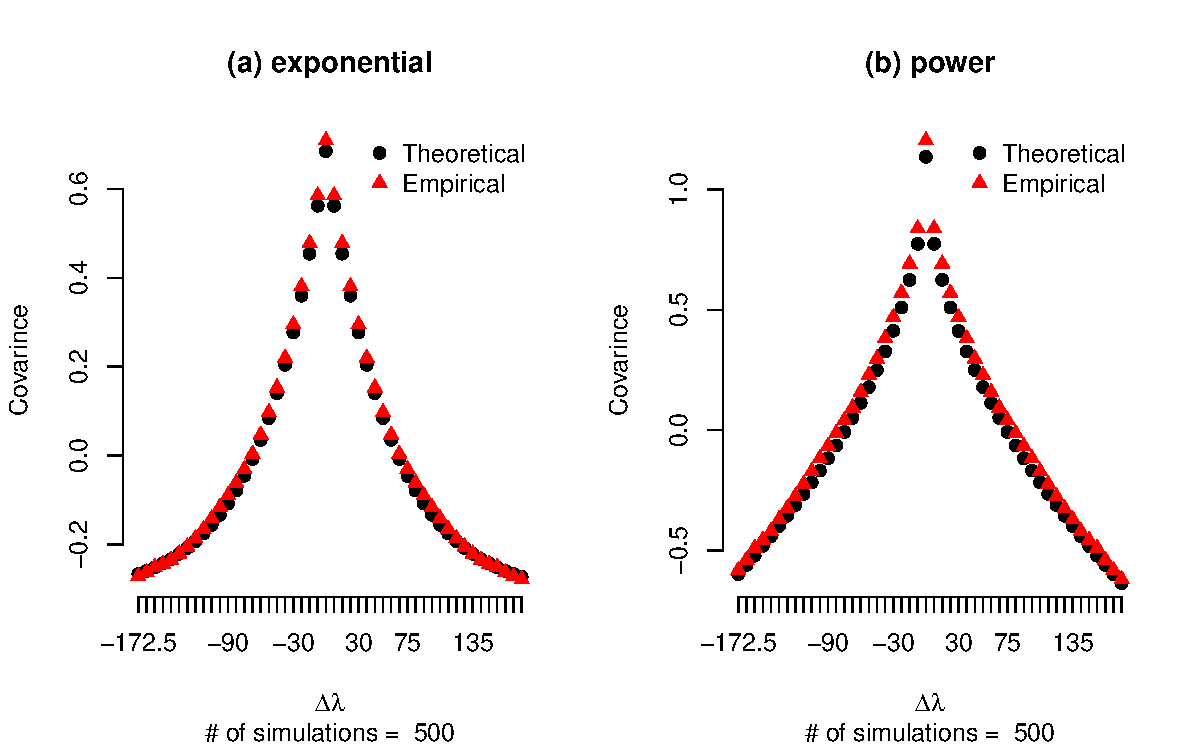
\includegraphics[width=0.8\textwidth]{graphs/covarince_circle_estimate_a0}
	 % \includegraphics[scale=.8, keepaspectratio]]{graphs/covarince_circle_estimate_a0}
	 %graph from data genaration summary doc line 194
	 \caption[Theoretical and Empirical Covariance Comparison on a Circle After]{Theoretical and empirical covariance comparison on a circle after substrating $\hat{a}_0$ from the empirical covariance.}
	 \label{covariance_estimate_a0}
	 \end{figure}
Now we theoretically calculate the unbiasedness of $\hat{C}(\Delta \lambda)$.
\begin{eqnarray*}
	E(\hat{C}(\Delta \lambda)) &=& \frac{1}{n}\sum_{i = 1}^n E((X(t_i + \Delta \lambda) - \bar{X})(X(t_i) - \bar{X})) \\
	&=& \frac{1}{n}\sum_{i = 1}^n E((X(t_i + \Delta \lambda) - \mu - (\bar{X} - \mu))(X(t_i) -\mu - (\bar{X}) - \mu)) \\
	&=& \frac{1}{n}\sum_{i=1}^n cov(X(t_i+\Delta \lambda), X(t_i)) - \frac{1}{n}\sum_{i = 1}^n E((X(t_i + \Delta \lambda) - \mu)(\bar{X} - \mu)) \\
	& & -\frac{1}{n}\sum_{i = 1}^n E((X(t_i) - \mu)(\bar{X} - \mu)) + \frac{1}{n}\sum_{i = 1}^n E((\bar{X} - \mu)(\bar{X} - \mu)) \\
	&=& C(\Delta \lambda) -E((\bar{X} - \mu)(\bar{X} - \mu)) - E((\bar{X} - \mu)(\bar{X} - \mu)) \\
	& & + E((\bar{X} - \mu)(\bar{X} - \mu)) \\
	&=& C(\Delta \lambda) - var(\bar{X}).
\end{eqnarray*}
That is, the MOM estimator $\hat{C}(\Delta \lambda)$ of the covariance function is actually a biased estimator with the shift amount approximately equal to $a_0$ it's still equal to $a_0$ even if a0=0. In other hand, if $a_0 = 0$, the MOM estimator $\hat{C}(\Delta \lambda)$ is an asymptotically unbiased estimator of $C(\theta)$. This leads to the following proposition

\pro{\label{prop3.2}
The MOM covariance estimator is a biased estimator of the true covariance function $C(\theta)$, if $a_0 > 0$. However, if $a_0 = 0$so that the process is a zero mean process then the MOM covariance estimator is asymptotically unbiased.
}

% \vskip 16pt

%-------------------------------------%
\section{Variogram MOM Estimator}
%-------------------------------------%

When the random process on a circle is stationary, the semivariogram can be obtained by
\[
\gamma(\theta) = C(0) - C(\theta).
\]
In $\R^n$, The variogram MOM estimator generally performs better than the covariance MOM estimator \citep{Cressie1993}. Given gridded data observations $\utilde{X}$, the variogram MOM estimator is given by
\beq
\hat{\gamma}(\Delta \lambda) = \frac{1}{2n} \sum_{i=1}^n (X(t_i + \Delta \lambda) - X(t_i))^2.
\eeq
We first perform a simulation with the same set up as before. Note that the theoretical exponential and power variogram functions are given below:
\begin{eqnarray*}
	\mbox{exponential : }\gamma(\theta) &=& C(0) - C(\theta) = C_1(1-e^{-a|\theta|}), \\
	\mbox{power : } \gamma(\theta) &=& C(0) - C(\theta) = (|\theta|/a)^{\alpha}.
\end{eqnarray*}
We compute the variogram estimator $\hat{\gamma}(\theta)$ with $n = 48$ gridded observations on the circle with 500 repetitions and then compared them with the theoretical values. The empirical and theoretical values match very well (Figure \ref{variogram_circle}).\\

\begin{figure}
	\centering
	%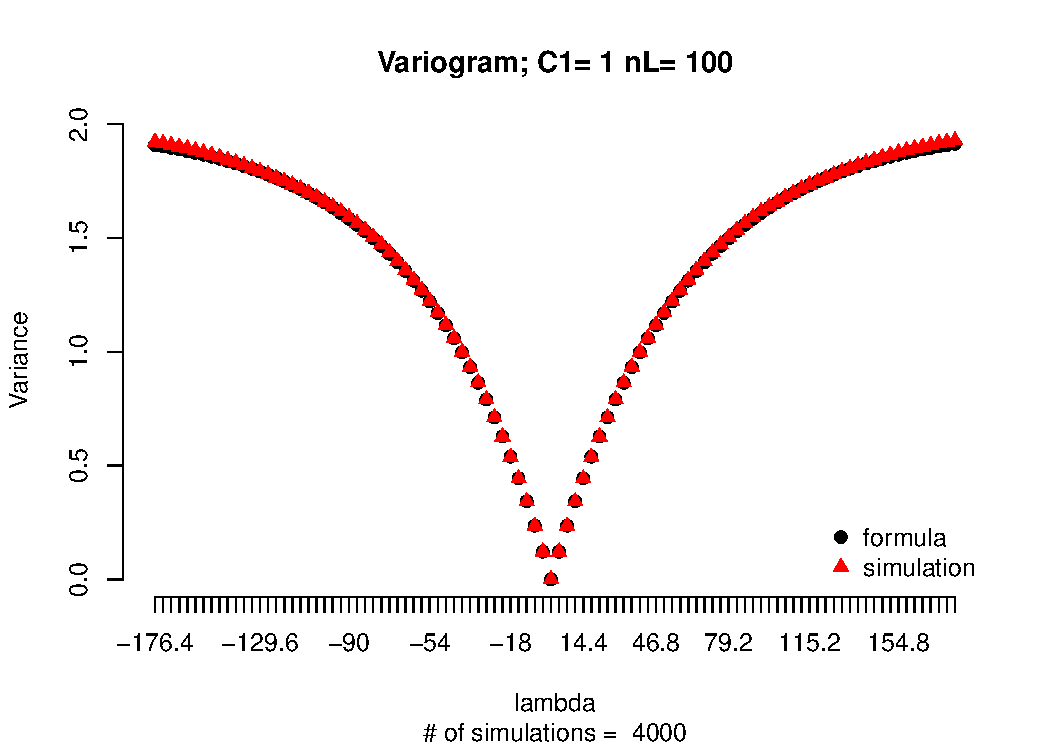
\includegraphics[width=0.65\textwidth]{graphs/variogram_plot_4000}
	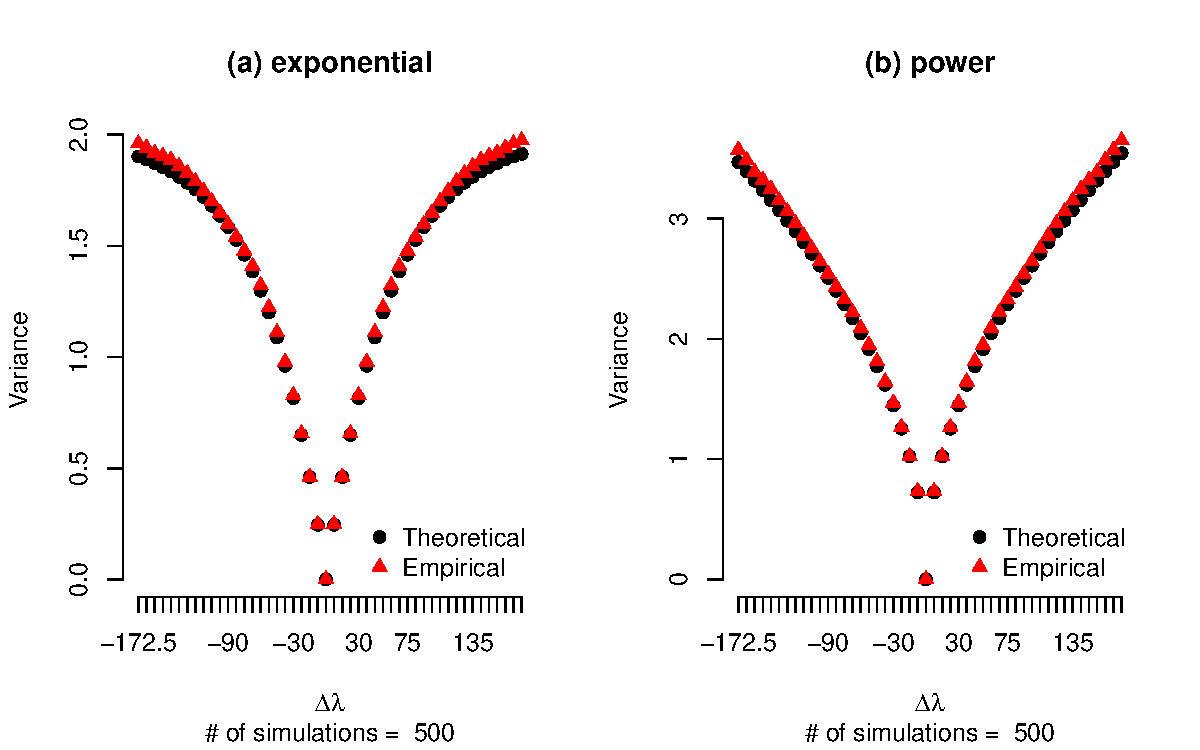
\includegraphics[width=0.9\textwidth]{graphs/variogram_plot_500}
	%graph from data genaration summary doc line 177
	\caption[Comparison Between Theoretical and Empirical Variogram on a Circle.]{Comparison between theoretical and empirical variogram on a circle.}
	\label{variogram_circle}
\end{figure}


Now we explore the asymptotics of the MOM variogram estimator.
% \begin{eqnarray}
% \nonumber
% E(\hat{\gamma}(\Delta \lambda)) &=&\frac{1}{2n} \sum_{i = 1}^n E(X(t_i + \Delta \lambda) - X(t_i))^2 \\
% \nonumber
% &=& \frac{1}{2n} \sum_{i = 1}^n E((X(t_i + \Delta \lambda)-\mu) - (X(t_i) - \mu))^2 \\
% \nonumber
% &=& \frac{1}{2n} \sum_{i = 1}^n cov(X(t_i + \Delta \lambda) - X(t_i), X(t_i + \Delta \lambda) - X(t_i)) \\
% \nonumber
% &=& \frac{1}{2n} \sum_{i = 1}^n \left(cov(X(t_i + \Delta \lambda), X(t_i + \Delta \lambda)) + cov(X(t_i), X(t_i))\right. \\
% \nonumber
% & & - \left. 2cov(X(t_i + \Delta \lambda), X(t_i)) \right)\\
% \nonumber
% &=& \frac{1}{2n} \sum_{i = 1}^n \left( C(0) + C(0) - 2C(\Delta \lambda)\right) \\
% &=& C(0) - C(\Delta \lambda) = \gamma(\Delta \lambda) \label{unbiased_variogram}.
% \end{eqnarray}
\begin{eqnarray}
\nonumber
E(\hat{\gamma}(\Delta \lambda)) &=&\frac{1}{2n} \sum_{i = 1}^n E(X(t_i + \Delta \lambda) - X(t_i))^2 \\
&=& \frac{1}{2n} \sum_{i = 1}^n \left( 2\gamma(\Delta \lambda)\right) = \gamma(\Delta \lambda) \label{unbiased_variogram}.
\end{eqnarray}
Therefore, $\hat{\gamma}(\Delta \lambda)$ is an unbiased estimator of $\gamma(\Delta \lambda)$.\\

We first calculate the variance and covariance of the variogram estimator on the circle. Again we consider the equal-distance gridded points on the circle $\{t_i: 1 \le i \le n, t_i = (i-1) \times 2\pi/n\}$ and $\utilde{X} = (X(t_1), X(t_2), \ldots, X(t_n))^T,$ being the observed data vectors. Assume that the random process $X(t)$ is stationary. $\hat{\gamma}(\Delta\lambda)$ can be written as
\[
\hat{\gamma}(\Delta \lambda) = \utilde{X}^T A(\Delta \lambda)\utilde{X}.
\]
Here for each $\Delta \lambda$, $A(\Delta \lambda)$ is a circulant matrix, and in particular, $A(0)= 0$. For simplicity, we set $n = 2N$ to be even. First we give an example for $n = 6$ to demonstrate the structure of $A(\Delta \lambda)$.\\

Let $n = 6$. For each of the four distance angles $\Delta \lambda = 0, \pi/3, 2\pi/3, \pi$, design matrices $A(\Delta \lambda)$ are given below:

\begin{eqnarray*}
A(0) &=& 0 ;  \\
A(\pi/3) &=& \frac{1}{12} \left(\begin{array}{cccccc}
2  &  -1 & 0  & 0 & 0 & -1 \\
-1 &  2  & -1 & 0 & 0 & 0   \\
0  & -1  & 2  & -1 & 0  & 0 \\
0  & 0   & -1 & 2  & -1 & 0 \\
0  & 0   &  0 & -1 & 2  & -1 \\
-1 & 0   &  0 &  0 & -1 & 2
\end{array}
\right) = \frac{1}{12} circ(2, -1, 0, 0, 0, -1);
\end{eqnarray*}
similarly,
\begin{eqnarray*}
A(2\pi/3) &=&  \frac{1}{12} circ(2, 0, -1, 0, -1, 0);\\
A(\pi) &=& \frac{1}{12} circ(2, 0, 0, -2, 0, 0).
\end{eqnarray*}
In general, for $1 \le m \le N-1$, and let $\delta = 2\pi/n$ be the common interval length so that $\Delta \lambda = m\delta$. Then we have
\begin{eqnarray*}
A(0) &=& 0; \\
A(m\delta) &=& \frac{1}{2n}circ(2, 0, 0, \ldots, -1, 0, \ldots, -1, 0, \ldots, 0), \\
& & \mbox{where $-1$'s are placed at $(m+1)^{th}$ and $(n-m+1)^{th}$ positions;} \\
A(N\delta) &=& A(\pi) = \frac{1}{2n}circ(2, 0, 0, \ldots, -2, 0, \ldots, 0),\\
& & \mbox{where $-2$ is placed at $(N+1)$th position.}
\end{eqnarray*}
It follows that $A(\Delta \lambda) = A(m\delta)$ is a symmetric circulant matrix. From Section 1.3, the eigenvalues of $A(m \delta)$ are then given by
\begin{eqnarray*}
\lambda_j^{(A)} &=& \frac{1}{2n}(2 - (\exp(j2\pi i/n))^m - (\exp(j2\pi i/n))^{n-m}) \\
&=& \frac{1}{2n}(2 - \exp(mj2\pi i/n) - \exp(-mj2\pi i/n)) \\
&=& \frac{1}{n}(1 - \cos(jm\lambda)) = \frac{1}{n}(1 - \cos(j\Delta \lambda)), \quad \quad j = 0, 1, 2, \ldots, n-1.
\end{eqnarray*}
for $1 \le m \le N-1$, and for $m = N$,
\begin{eqnarray*}
\lambda_j^{(A)} &=& \frac{1}{2n}(2 - 2 (\exp(j2\pi i/n))^{N}) \\
 &=& \frac{1}{n}(1 - \cos(j\pi)) \\
 &=& \frac{1}{n}(1 - \cos(j\Delta \lambda)), \quad \quad j = 0, 1, \cdots, n-1.
\end{eqnarray*}
In addition, from Section \ref{circulant}, all circulant matrices can be orthogonally diagonalized using the same orthogonal (Fourier) matrix, denoted as $P$. Consequently,
the trace of the product of circulant matrices is the trace of product of diagonal matrices, which is the sum of the product of corresponding eigenvalues from those circulant matrices. \\

Next we consider the distribution of the variogram estimator. First we write the variogram estimator in the following form:
\begin{eqnarray*}
\hat{\gamma}(\Delta \lambda) &=& \frac{1}{2n} \sum_{i=1}^n (X(t_i + \Delta \lambda) - X(t_i))^2  \\
&=& \frac{1}{2n} \sum_{i=1}^n ((X(t_i + \Delta \lambda)-\mu) - (X(t_i)-\mu))^2.
\end{eqnarray*}
\noi Therefore,
\beq
\hat{\gamma}(\Delta \lambda) = (\utilde{X}-\utilde{\bf 1}_n\mu)^T A(\Delta \lambda)(\utilde{X}-\utilde{\bf 1}_n\mu).
\eeq
Note that $A(\Delta \lambda)$ is a circulant matrix with following spectral decomposition
\begin{eqnarray*}
A(\Delta \lambda) &=& P \Lambda^{(A)}P^T,
\end{eqnarray*}
where $P$ is the Fourier matrix (orthonormal), solely depending on the dimension of $A$, and
\begin{eqnarray*}
\Lambda^{(A)} &=& \mbox{diag}(\lambda_1^{(A)}, \lambda_2^{(A)}, \cdots, \lambda_n^{(A)}), \\
\mbox{with} \quad \lambda_m^{(A)} &=& \frac{1}{n}(1 - \cos((m-1)\Delta \lambda)), \quad \quad m = 1, 2, \cdots, n.
\end{eqnarray*}
If $\utilde{X}$ follows a multivariate normal distribution $N(\utilde{\bf 1}_n\mu, \Sigma)$, then $(\utilde{X}-\utilde{\bf 1}_n\mu) \sim N(\utilde{\bf 0}, \Sigma)$. Note that
the variance-covariance matrix $\Sigma$ is also a circulant matrix, which has the following spectral decomposition:
\begin{eqnarray*}
\Sigma &=& P \Lambda^{(\Sigma)} P^T,\\
\mbox{with}\quad \Lambda^{(\Sigma)} &=& \mbox{diag}(\lambda_1^{(\Sigma)}, \lambda_2^{(\Sigma)}, \cdots, \lambda_n^{(\Sigma)}),
\end{eqnarray*}
\begin{flalign*}
\text{where } \quad \lambda_j^{(\Sigma)} &= \left(C(0) + 2\sum_{m = 1}^{N-1}C(m\delta)\cos((j-1)m\delta) + C(\pi)\cos((j-1)N\delta)\right).
\end{flalign*}
Let $\utilde{Y} = P^T\left(\utilde{X} - \utilde{\bf 1}_n \mu \right)$, then $\utilde{Y}$ follows a multivariate normal distribution with mean $\utilde{\bf 0}$ and variance-covariance matrix given by
\begin{eqnarray*}
var(\utilde{Y}) &=& cov(P^T\left(\utilde{X} - \utilde{\bf 1}_n \mu \right), P^T\left(\utilde{X} - \utilde{\bf 1}_n \mu \right)) \\
&=& P^T \Sigma P  = P^T P \Lambda^{(\Sigma)} P^T P = \Lambda^{(\Sigma)}.
\end{eqnarray*}
That is, $\utilde{Y} \stackrel{\triangle}{=} (Y_1, Y_2, \cdots, Y_n)^T$ are independent normal random variates with mean 0 and variance $\lambda_j^{(\Sigma)}$, $j=1,2,\ldots,n$, respectively. \\

The variogram estimator is then given by
\begin{eqnarray*}
\hat{\gamma}(\Delta \lambda) &=& (\utilde{X}-\utilde{\bf 1}_n\mu)^T A(\Delta \lambda)(\utilde{X}-\utilde{\bf 1}_n\mu) \\
&=& (P(\utilde{X}-\utilde{\bf 1}_n\mu))^T \Lambda^{(A)} (P^T(\utilde{X}-\utilde{\bf 1}_n\mu))  \\
&=& \utilde{Y} \Lambda^{(A)} \utilde{Y} = \sum_{m = 1}^n \lambda_m^{(A)} Y_m^2.
\end{eqnarray*}
Note that $\frac{Y_m}{\sqrt{\lambda_m^{(\Sigma)}}} \sim N(0, 1)$, and so $\frac{Y_m^2}{\lambda_m^{(\Sigma)}} \sim \chi_1^2$ (or written as $\chi_{1, m}^2$ due to the dependency on $m$), which implies
\begin{eqnarray*}
\hat{\gamma}(\Delta \lambda) &=& \sum_{m = 1}^n \lambda_m^{(A)} \lambda_m^{(\Sigma)} \left(\frac{Y_m}{\sqrt{\lambda_m^{(\Sigma)}}}\right)^2 \stackrel{\triangle}{=} \sum_{m = 1}^n \lambda_m^{(A)} \lambda_m^{(\Sigma)} \chi_{1,m}^2.
\end{eqnarray*}
Here $\chi_{1, 1}^2, \chi_{1, 2}^2, \cdots, \chi_{1, n}^2$ are {\em i.i.d.} $\chi_1^2$ random variables. Hence
\[
E(\hat{\gamma}(\Delta \lambda)) = \sum_{m = 1}^n \lambda_m^{(A)} \lambda_m^{(\Sigma)}, \quad \quad var(\hat{\gamma}(\Delta \lambda)) = 2 \sum_{m = 1}^n (\lambda_m^{(A)} \lambda_m^{(\Sigma)})^2
\]
that
\[
E(\hat{\gamma}(\Delta \lambda)) = \sum_{m = 1}^n \lambda_m^{(A)} \lambda_m^{(\Sigma)} = \gamma(\Delta \lambda),
\]
which recovers the result\eqref{unbiased_variogram} we obtained earlier. Next we consider the variance of the variogram estimator under the Gaussian assumption. \\

Without loss of generality, we assume that $a_1 > 0$ (otherwise, we can always choose some $a_m$ such that $a_m > 0$). First notice that
\begin{eqnarray*}
\hat{\gamma}(\Delta \lambda) &=& \sum_{m = 1}^n \lambda_m^{(A)} \lambda_m^{(\Sigma)} \chi_{1,m}^2  \\
&=& (C(0) - C(\Delta \lambda)) \sum_{m = 1}^n \frac{\lambda_m^{(A)} \lambda_m^{(\Sigma)}}{C(0) - C(\Delta \lambda)} \chi_{1,m}^2  \\
&\overset{\bigtriangleup}{=}&  (C(0) - C(\Delta \lambda)) \sum_{m = 1}^n C_{n,m} \chi_{1,m}^2,
\end{eqnarray*}
where $\sum_{m=1}^n C_{n, m} = \sum_{m=1}^n \frac{\lambda_m^{(A)} \lambda_m^{(\Sigma)}}{C(0) - C(\Delta \lambda)} = 1$ and $C_{n, m} > 0$ since both the matrices $A$ and $\Sigma$ are positive definite. Hence
\begin{eqnarray*}
var(\hat{\gamma}(\Delta \lambda)) &=& (C(0) - C(\Delta \lambda))^2 * 2 * \left(\sum_{m = 1}^n C_{n,m}^2\right) \\
&\le& 2(C(0) - C(\Delta \lambda))^2\left(\sum_{m = 1}^n C_{n,m}\right) = 2(C(0) - C(\Delta \lambda))^2.
\end{eqnarray*}
On the other hand,
\begin{eqnarray*}
var(\hat{\gamma}(\Delta \lambda)) &=& (C(0) - C(\Delta \lambda))^2 * 2 * \left(\sum_{m = 1}^n C_{n,m}^2\right) \\
&\ge& (C(0) - C(\Delta \lambda))^2 * 2 * C_{n, 2}^2.
\end{eqnarray*}
Note that
\begin{eqnarray*}
C_{n, 2} &=& \frac{1 - \cos(\Delta \lambda)}{C(0) - C(\Delta \lambda)} \frac{1}{n}\left(C(0) + 2\sum_{k = 1}^{N-1}C(k\delta)\cos(k\delta) + C(\pi)\cos(N\delta)\right) \\
&=& \frac{1 - \cos(\Delta \lambda)}{C(0) - C(\Delta \lambda)} \frac{1}{\pi} \frac{\pi}{n}\left(C(0) + 2\sum_{k = 1}^{N-1}C(k\delta)\cos(k\delta) + C(\pi)\cos(N\delta)\right).
\end{eqnarray*}
Now we consider the limit of $C_{n, 2}$ when $n \to \infty$. It should be pointed out that when $n \to \infty$, we are sampling denser and denser data points over the circle so that we have $\Delta\lambda$ obtainable. A simple approach is to take the sample size $n$ to be doubled so that $n$ tends to infinity while maintaining $\gamma(\Delta \lambda)$ to be estimable. Under this setting, we have
\begin{eqnarray*}
\frac{\pi}{n}\left(C(0) + 2\sum_{k = 1}^{N-1}C(k\delta)\cos(k\delta) + C(\pi)\cos(N\delta)\right) \to \int_0^\pi C(\theta)\cos(\theta)d\theta, \quad \mbox{as $n \to \infty$},
\end{eqnarray*}
and so
\begin{eqnarray*}
C_{n, 2} &\to& \frac{1 - \cos(\Delta \lambda)}{C(0) - C(\Delta \lambda)} \frac{1}{2} \frac{2}{\pi}\int_0^\pi C(\theta)\cos(\theta)d\theta = \frac{1 - \cos(\Delta \lambda)}{C(0) - C(\Delta \lambda)}*\frac{a_1}{2}, \\
C_{n, 2} &>& \frac{1 - \cos(\Delta \lambda)}{C(0) - C(\Delta \lambda)}*(\frac{a_1}{2} - \varepsilon_0),
\end{eqnarray*}
for a fixed $0 < \varepsilon_0 < \frac{a_1}{2}$ and a large enough sample size $n$. Consequently,
\begin{eqnarray*}
var(\hat{\gamma}(\Delta \lambda)) &>& 2(a_1/2 - \varepsilon_0)^2(1 - \cos(\Delta \lambda))^2.
\end{eqnarray*}
We summary our findings as the following proposition.

\pro{
The variance of the variogram MOM estimator is finite and asymptotically bounded away from zero.
}

From our previous calculation, we have, for each fixed $m$,
\begin{eqnarray*}
C_{n, m} &=& \frac{1}{n}(1 - \cos((m-1)\Delta \lambda)) \\
& &\left(C(0) + 2\sum_{k = 1}^{N-1}C(k\delta)\cos((m-1)k\delta) + C(\pi)\cos((m-1)\pi)\right)/(C(0)-C(\Delta \lambda)) \\
& \to & (1 - \cos((m-1)\Delta \lambda)) \left(\frac{1}{\pi}\int_0^\pi C(\theta)\cos((m-1)\theta)d\theta\right)/(C(0)-C(\Delta \lambda)) \\
&=& {a_{m-1}}{2}(1 - \cos((m-1)\Delta \lambda))/(C(0)-C(\Delta \lambda)), \quad \mbox{as $n \to \infty$.}
\end{eqnarray*}
Now we present our main result for the MOM variogram estimator.

\pro{
If the underlying process $X(t)$ is assumed to be Gaussian, the MOM variogram estimator is not consistent on the circle.
}

\begin{proof}
First we consider the consistency of the variogram estimator. To show the following
\[
P\left( \left|\hat{\gamma}(\Delta \lambda) - \gamma(\Delta \lambda)\right| \ge \varepsilon\right) \to 0,
\]
as $n \to \infty$ for fixed $\varepsilon > 0$ and $\Delta \lambda \ne 0$, it is equivalent to show that
\[
P\left( \left|\sum_{m = 1}^n C_{n, m} \chi_{1, m}^2 - 1 \right| \ge \varepsilon\right) \to 0,
\]
as $n \to \infty$ for fixed $\varepsilon > 0$ and $\Delta \lambda \ne 0$. Here $\sum_{m=1}^n C_{n, m} = 1, C_{n, m} > 0$ for each fixed $n$. Note that we also have, for each fixed $m$,
\[
0 < C_{n, m} \to \frac{a_m}{2}\frac{1 - \cos(m \Delta \lambda)}{C(0) - C(\Delta \lambda)} \equiv b_m.
\]
For simplicity, we can assume that $b_2 > 0$ (Otherwise we can pick some $b_m > 0$ for some $m$ fixed). That is
\[
C_{n, 2} \to b_2 > 0, \quad \quad \mbox{as $n \to \infty$}.
\]
Therefore, for fixed $\varepsilon_0 > 0$ and $\varepsilon_0 < b_2$, we choose all $n > N$, such that
\[
b_2 - \varepsilon_0 < C_{n, 2} < b_2 + \varepsilon_0
\]
Therefore, for all $n > N$, (and denote $\chi_{1, 2}^2 = \chi_1^2$ for simplicity)
\[
\sum_{m = 1}^n C_{n, m}\chi_{1,m}^2  \ge  C_{n, 2} \chi_{1, 2}^2 > (b_2 - \varepsilon_0) \chi_1^2
\]
. Hence notice that, for the fixed $\varepsilon > 0$,
\[
\left\{(b_2 - \varepsilon_0) \chi_{1}^2 > 1 + \varepsilon  \right\} \subseteq \left\{\sum_{m = 1}^n C_{n, m}\chi_{1,m}^2 > 1 + \varepsilon  \right\}
\]
Now, for all $n \ge N$,
\begin{eqnarray*}
& & P\left( \left|\sum_{m = 1}^n C_{n, m} \chi_{1, m}^2 - 1 \right| \ge \varepsilon\right) \\
&=& P\left( \sum_{m = 1}^n C_{n, m} \chi_{1, m}^2 > 1 + \varepsilon \quad \mbox{or} \quad  \sum_{m = 1}^n C_{n, m} \chi_{1, m}^2 < 1 - \varepsilon\right) \\
& \ge & P\left( \sum_{m = 1}^n C_{n, m} \chi_{1, m}^2 > 1 + \varepsilon \right)  \ge  P\left((b_2 - \varepsilon_0) \chi_{1}^2 > 1 + \varepsilon  \right) \\
& = & P\left(\chi_{1}^2 > \frac{1 + \varepsilon}{b_2 - \varepsilon_0}\right) \not\to 0,
\end{eqnarray*}
since the last term is a fixed positive number. This proves the non-consistency of variogram estimator.

\end{proof}



% \end{document}





%%------------------------------------------------------------------%%
\chapter{Parametric Models on a Sphere}
%\documentclass[12pt, amstex, letterpaper] {report} %{article}


\usepackage[margin=1in]{geometry}
\topmargin -0.5in \textwidth 6.5in \textheight 9in
\footskip .5in
\headheight 0.3in


\usepackage{Sweave}

\DefineVerbatimEnvironment{Sinput}{Verbatim} {xleftmargin=0em,frame=single}
\DefineVerbatimEnvironment{Soutput}{Verbatim} {xleftmargin=0em,frame=single}

\usepackage{amssymb, mathrsfs, amsmath, amsfonts}
\usepackage{enumerate, comment}
\usepackage{hyperref, natbib,apalike, float} %cite
\usepackage{color, multirow, setspace, fancyhdr,graphicx}
\usepackage{undertilde}
\usepackage[bottom]{footmisc}
\usepackage{graphicx}
\usepackage{framed}
\usepackage{subcaption}
\usepackage{amsthm}

%\doublespacing
\pagestyle{empty}
\pagestyle{fancy}
\lhead{ }
%\rhead{May 2016}
\fancyfoot{ }
\rfoot{Dissertation $|$ \thepage}
\lfoot{Chris Vanlangenberg}
\date{}

\includecomment{comment}

\newtheorem{theorem}{Theorem}[section]
\newtheorem{defn}{Definition}[section]
\newtheorem{prop}{Proposition}
\newcommand{\pro}[1]{\begin{prop}{#1}\end{prop}}

%\newtheorem{proof}{proof}
\newtheorem{rmk}{Remark}
\newcommand{\rmark}[1]{\begin{rmk}{#1}\end{rmk}}

\numberwithin{equation}{section}
\renewcommand{\footrulewidth}{0.1pt}
\renewcommand{\headrulewidth}{0.1pt}


\newcommand{\eqn}[1]{\begin{equation}{#1}\end{equation}}

\newcommand{\beq}{\begin{equation}}
\newcommand{\eeq}{\end{equation}}
%\renewcommand\refname{Literature}
\newcommand{\blue}[1]{\textcolor{blue}{\emph{#1}}}
\newcommand{\red}[1]{\textcolor{red}{\emph{#1}}}
\newcommand{\twoc}[2]{{\textcolor{blue}{#1}} and {\textcolor{red}{#2}}}


\newcommand{\xn}{x_1,\ldots, x_n}
\newcommand{\Xn}{X_1,\ldots, X_n}
\newcommand\floor[1]{\lfloor{#1}\rfloor}
\newcommand\ceil[1]{\lceil{#1}\rceil}

\newcommand{\X}{\mathcal{X}}
\newcommand{\Sp}{\mathbb{S}}
\newcommand{\R}{\mathbb{R}}
\newcommand{\C}{\mathbb{C}}
\newcommand{\pd}{positive definite }



\newcommand{\code}[1]{{\small\texttt{#1}}}
\newcommand{\pkg}[1]{{\normalfont\textsf{#1}}}
\newcommand{\var}[1] {{\normalfont\textbf{#1}}}
\newcommand{\Cm}{$C_m(\phi_P, \phi_Q)\ $}

\newcommand{\jun}{\cite{JunStein2008}}
%
%\begin{document}


%%-------------------------Random process on sphere---------------------------------------%%

%%------------------------------------------------------------------%%
\section{Random Process on a Sphere}
%%------------------------------------------------------------------%%
	
Suppose the process $\{X(P): P\in \Sp^2\}$ ($\Sp^2$ unit sphere), defined in a common probability space, where $P=(\lambda, \phi) \in \Sp^2$ with longitude $\lambda \in [-\pi, \pi)$ and latitude $\phi \in [0, \pi]$, is continuous in quadratic mean with respect to the location $P$ and has finite second moment. Then it can be represented by spherical harmonics \citep{Jones1963, LiNorth1997, Huang2012}, with the sum converging in mean squares:
	\[
	X(P) = \sum_{\nu=0}^\infty \sum_{m=-\nu}^{\nu} Z_{\nu,m} e^{i m \lambda} P_{\nu}^m (\cos \phi).
	\]
Here $P_{\nu}^m(\cdot)$ are normalized associated Legendre polynomials such that their squared integral on $[-1, 1]$
is 1, and $Z_{\nu,m}$ are complex-valued coefficients satisfying	
	\[
	Z_{\nu,m} = \int_{\Sp^2} X(P) e^{-im \lambda} P_{\nu}^m (\cos \phi) d P.
	\]
Without loss of generality, we suppose that the process $X(P)$ is with zero mean, which implies $E(Z_{\nu,m}) = 0$. Let $P = (\lambda_P, \phi_P)$ and $Q=(\lambda_Q, \phi_Q)$ be two arbitrary locations on the sphere, the covariance function of the process is given by
	\begin{eqnarray*} \label{rpq_1}
		R(P, Q) &=& \mbox{E}(X(P) \overline{X(Q)}) \\
		&=& \sum_{\nu=0}^\infty \sum_{\mu=0}^\infty \sum_{m=-\nu}^{\nu} \sum_{n=-\mu}^{\mu} \mbox{E}(Z_{\nu,m} \overline{Z}_{\mu,n}) e^{im \lambda_P} P_{\nu}^m(\cos \phi_P) e^{-i n \lambda_Q} P_{\mu}^n (\cos \phi_Q),
	\end{eqnarray*}
where $\bar{Z}$ denotes the complex conjugate of $Z$. Note that the continuity of $X(P)$ on every point $P$ implies that $R(P, Q)$ is continuous at all pairs of $(P, Q)$ \citep[page 83]{Leadbetter1967}.

	%%------------------------------------------------------------------%%
	\subsection{Homogeneous Covariance Functions on the Sphere}
	%%------------------------------------------------------------------%%
	
Under the assumption of homogeneity (or isotropy), the covariance function of a random process $X(\cdot)$ on $\Sp^2$ is invariant under rotations. More specifically, a homogeneous random process on the sphere satisfies
	\begin{eqnarray*}
	E(X(P)) &=& \mu, \quad \mbox{for any } P \in \Sp^2, \\
		Cov(X(P),X(Q)) &=& C(\theta_{PQ}),
	\end{eqnarray*}
where $\theta_{PQ}$ is the spherical angle between two locations $P, Q$, given by 
	\begin{eqnarray*}
		\theta_{PQ}  = \arccos\left(\sin(\phi_P)\sin(\phi_Q) + \cos(\phi_P)\cos(\phi_Q)\cos(\lambda_P-\lambda_Q)\right).
	\end{eqnarray*}
Parallel to the requirement for a valid covariance function in $\R^d$, a valid covariance function $C(\cdot)$ on the sphere must be non-negative definite, {\em i.e.,}
	\begin{eqnarray*}
	\sum_{i,j=1}^{N} a_i a_j C(\theta_{P_iP_j}) \ge 0,
    \end{eqnarray*}
for any integer $N$, any constants $a_1, a_2, \ldots, a_N$, and any locations $P_1, P_2, \ldots, P_N \in \Sp^2$. \\

According to \cite{schoenberg1942}, a real continuous function $C(\theta)$ is a valid homogeneous covariance function on the sphere ($\Sp^2$) if and only if it can be written in the following form:
	\begin{eqnarray*} \label{covs2_sum}
	C(\theta) = \sum_{k = 0}^\infty c_k P_k(\cos\theta), \quad \theta \in [0,\pi],
	\end{eqnarray*}
where $P_k(\cdot)$ is the Legendre polynomial, $\forall c_k\ge 0$ and $\sum_k c_k < \infty$. A general result of the above representation on $\Sp^d\ (d > 2)$ can also be found in \cite{schoenberg1942}. \\
	
Note that the Legendre polynomials $P_k(\cdot)$ are orthogonal in the following sense:
	\[
		\int_{-1}^{1} P_{n}(x)P_{m}(x)dx = \frac{2}{2n+1}\delta_{(n,m)}.
	\]
Hence the coefficients $c_k$ can be obtained as
	\beq \label{covs2_coef}
	c_{k} = \frac{2k+1}{2}\int_0^{\pi} C(\theta)P_{k}(\cos\theta)d\theta. \quad k = 0,1,2,\ldots
	\eeq
One can directly use the above integral to evaluate the validity of a homogenous covariance function on the sphere by checking if $c_k$ is non-negative for all k and $\sum_k c_k < \infty$ . \\
	
The construction of covariance models is critical for spatial prediction. However, the covariance models that are valid on $\R^d$ may not be valid on the sphere ($\Sp^2$). For example, \cite{HuangZhangRobeson2011} evaluated the validity of commonly used \cov models that are valid on $\R^d$ and summarized their findings in Table \ref{tab:cov_sphere}.

	\begin{table}[H]
		\label{valid_cov_models}
		\centering
		\caption [Validity of Covariance Functions on the Sphere]{Validity of covariance functions on the sphere, $a >0,\theta \in [0,\pi]$}
		\label{tab:cov_sphere}
		\vskip 16pt
		\begin{tabular}[htb]{lll} \hline \hline
			Model & Covariance function & Valid on $\Sp^2$           \\   \hline Spherical  &
			$\left(1-\frac{3\theta}{2a} + \frac{1}{2}
			\frac{\theta^3}{a^3}\right){\bf 1}_{(\theta \le a)}$ & Yes   \\
			[2ex]
			Stable     & $\exp\left\{-\left(\frac{\theta}{a}\right)^\alpha\right\}$ & Yes for $\alpha \in (0,1]$  \\
			      &                     & No for $\alpha \in (1,2]$ \\ [2ex] \hspace{0.2in} Exponential &
			$\exp \{-\left(\frac{\theta}{a}\right) \}$ & Yes \\ [2ex]
			\hspace{0.2in} Gaussian & $\exp\left\{-\left(\frac{\theta}{a} \right)^2
			\right\}$  & No \\ [2ex]
			Power$^*$  & $c_0 - (\theta/a)^\alpha$ & Yes for  $\alpha \in (0,1] $  \\
			& & No for $\alpha \in (1,2]$ \\ [2ex]
			Radon transform of order 2         & $e^{-\theta/a}(1+\theta/a)$ &
			No        \\ [2ex] Radon transform of order 4         &
			$e^{-\theta/a} (1+\theta/a+\theta^2/3a^2)$  & No  \\ [2ex] Cauchy &
			$(1+\theta^2/a^2)^{-1}$ &  No      \\ [2ex] Hole - effect & $\sin
			a\theta / \theta$ & No    \\ \hline \hline
		\end{tabular}
	\vskip 8pt	
$^*$When $\alpha \in (0,1]$, the power model is valid on the sphere  for some $c_0 \ge \int_0^\pi (\theta/a)^{\alpha} \sin \theta d \theta$.
		\end{table}
		 
Furthermore, \cite{Gneiting2013} showed that the Mat$\acute{e}$rn covariance function is only valid on the sphere when the smoothness parameter $\nu\in(0,1/2]$. Another way of constructing a valid homogeneous covariance function on the sphere is by using the valid covariance function in $\R^3$. Specifically, \cite{Yadrenko1983} showed that if $K(\cdot)$ is a valid isotropic covariance function on $\R^3$ then
\[
	C(\theta) = K(2\sin(\theta/2))
\]
is a valid isotropic covariance function on the unit sphere, where $\theta$ is the greatest circle distance on the sphere.
			
		%%------------------------------------------------------------------%%
		\subsection{Variogram on a Sphere}
		%%------------------------------------------------------------------%%
			
Parallel to the case of circle, if a random process $X(\cdot)$ on a sphere is intrinsically stationary on $\Sp^2$, then one has $E(X(P))=\mu$, an unknown constant for all $P\in \Sp^2$ and the variogram function between any two locations $P, Q \in \Sp^2$ depends only on the spherical angle $\theta_{PQ}$	
		\[
			Var(X(P)-X(Q)) = 2\gamma(\theta_{PQ}), \quad \forall P, Q \in \Sp^2.
		\]
		The variogram function is conditionally negative definite, that is,
		\[
			\sum_{i,j=1}^{N} a_i a_j 2\gamma(\theta_{P_iP_j}) \le 0,
		\]
for any integer $N$, any constants $a_1, a_2, \ldots, a_N$ with $\sum_i a_i = 0$, and any locations $P_1, P_2, \ldots P_N \in \Sp^2$. Immediately from \eqref{covs2_sum}, for a continuous function $2\gamma(\cdot)$ with $\gamma(0)=0$, the variogram is negative definite if and only if
		\beq
		\gamma(\theta) = \sum_{k = 0}^\infty c_k(1-P_k(\cos\theta)), \quad \theta \in [0,\pi]
		\eeq
where $P_{k}(\cdot)$ are Legendre polynomials, $\forall c_k\ge 0$ and $\sum c_k < \infty$. \\
			
It is known that in $\R^d$, one can always obtain the variogram from the stationary covariance function with $\gamma(\theta) = C(0) - C(\theta)$ but not the converse. However, in $\Sp^2$ \cite{Yaglom1961} argued that for a valid $\gamma(\theta), \theta \in [0,\pi]$ one can always construct the covariance function $C(\theta)=c_0-\gamma(\theta)$ for some $c_0 \ge \int_0^{\pi} \gamma(\theta)\sin(\theta)d\theta$. \\
			
Here is the outline of this chapter. We first introduce axially symmetric random processes on the sphere and the representation for the covariance function. Next, we propose parametric models to generalize some of existing parametric models to capture the variation across latitudes when modeling the covariance structure of axially symmetric processes on the sphere. Finally, we discuss the properties of the cross-covariance and cross-variogram estimators based on the Method of Moments.
		
\vskip 8pt		
		%%------------------------------------------------------------------%%
		\section{Axial Symmetry}
		%%------------------------------------------------------------------%%

For an axially symmetric process $X(P), P \in \Sp^2$ on the sphere, the covariance function $R(P,Q)$ at two locations $P=(\phi_P, \lambda_P), Q=(\phi_Q,\lambda_Q) \in \Sp^2$ is given by 					 
\[
R(\phi_P, \phi_Q, \lambda_P, \lambda_Q) = R(\phi_P, \phi_Q, \lambda_P-\lambda_Q).
\]
Following the discussion given by \cite{Stein2007, Huang2012}, the covariance function can be expressed as the following:					
		\begin{eqnarray} \label{axially-symmetry-cov}
			R(P,Q)  & = & R(\phi_P, \phi_Q, \lambda_P-\lambda_Q) \nonumber \\
			& = & \sum_{m=-\infty}^{\infty} \sum_{\nu=|m|}^\infty \sum_{\mu=|m|}^\infty f_{\nu,\mu,m} e^{im (\lambda_P-\lambda_Q)} P_{\nu}^m(\cos \phi_P) P_{\mu}^m (\cos \phi_Q),
		\end{eqnarray}
where the matrix $F_m(N) = \{ f_{\nu,\mu,m} \}_{\nu,\mu=|m|,|m|+1, \ldots, N }$ must be positive definite for all $N \ge |m|$ and $f_{\nu,\mu, m} = \overline{f}_{\mu, \nu, m}$ for each fixed integer $m$. Furthermore, if we denote
\[
C_m(\phi_P, \phi_Q) = \sum_{\nu=|m|}^\infty \sum_{\mu=|m|}^\infty f_{\nu,\mu,m} P_{\nu}^m(\cos \phi_P) P_{\mu}^m (\cos \phi_Q),
\]
then 				
		\beq \label{R(PQ)-01}
		R(P,Q) = R(\phi_P,\phi_Q,\Delta\lambda) = \sum_{m = -\infty}^{\infty}e^{im\Delta\lambda}C_m(\phi_P,\phi_Q), \quad m=0, \pm 1, \pm 2,...,
		\eeq
where $\Delta\lambda = \lambda_P - \lambda_Q \in [-\pi, \pi]$ and $\phi_P, \phi_Q \in [0,\pi]$. Here the complex bivariate continuous function \Cm has the following properties:

		\begin{itemize}
			\item Hermitian and positive definite.
			\item $\sum_{m = -\infty}^{\infty}|C_m(\phi_P,\phi_Q)|<\infty$ for any $\phi_P, \phi_Q \in [0, \pi]$.
		\end{itemize}
One can use the inverse Fourier transformation to derive $C_m(\phi_P, \phi_Q)$ based on $R(P,Q)$, 				
		\[
			C_m(\phi_P, \phi_Q) = \frac{1}{2\pi}\int_{-\pi}^{\pi} R(\phi_P, \phi_Q, \Delta\lambda)e^{-im\Delta\lambda} d\Delta\lambda. 
        \]
Let $C_m(\phi_P, \phi_Q) = C_m^R(\phi_P, \phi_Q) + i C_m^I(\phi_P, \phi_Q)$. From \cite{Huang2012}, if a random process is real-valued, its corresponding covariance function $R(P,Q)$ is also real-valued, and so we have \Cm $= \overline{C_{-m}(\phi_P,\phi_Q)}$. The covariance function $R(P,Q)$ on the sphere given by \eqref{R(PQ)-01} can then be simplified as the following:
			\begin{eqnarray*}
				R(P,Q) &=& C_0(\phi_P,\phi_Q) + \sum_{m=1}^{\infty} e^{-im\Delta\lambda}C_{-m}(\phi_P,\phi_Q) +  \sum_{m=1}^{\infty} e^{im\Delta\lambda}C_m(\phi_P,\phi_Q) \\
				% &=& C_0(\phi_P,\phi_Q) + \sum_{m=1}^{\infty} c_m e^{-im\Delta\lambda}( C_m^{R}(\phi_P,\phi_Q) - i C_m^{I}(\phi_P,\phi_Q)) \\
				% & &  + \sum_{m=1}^{\infty}c_m e^{im\Delta\lambda}( C_m^{R}(\phi_P,\phi_Q) + iC_m^{I}(\phi_P,\phi_Q)) \\
				&=& C_{0}^{R}(\phi_P,\phi_Q)+2 \sum_{m=1}^{\infty}[\cos(m\Delta\lambda)C_{m}^{R}(\phi_P,\phi_Q)-\sin(m\Delta\lambda)C_{m}^{I}(\phi_P,\phi_Q)].
			\end{eqnarray*}
			
			
			%%------------------------------------------------------------------%%
			\subsection{Longitudinally Reversible Processes}
			%%------------------------------------------------------------------%%
If we further assume that the covariance function $R(P, Q)$ of an axially symmetric process satisfies
			\beq
			R(\phi_P, \phi_Q, \lambda_P-\lambda_Q) = R(\phi_P, \phi_Q, \lambda_Q-\lambda_P),
			\eeq
we then call the underlying process to be longitudinally reversible (\cite{Stein2007}). Now the covariance function $R(P, Q)$ of a real-valued longitudinally reversible process reduces to			
			\[
				R(P,Q) = \sum_{m=0}^{\infty} C_m(\phi_P,\phi_Q)\cos(m\Delta\lambda).
			\]
as \Cm is real so that we have $C_{-m}(\phi_P,\phi_Q)=C_m(\phi_P,\phi_Q)$  and \Cm $= \overline{C_{-m}(\phi_P,\phi_Q)}$.

\vskip 16pt
				
%%------------------------------------------------------------------%%
\section{Proposed Parametric Models}
%%------------------------------------------------------------------%

As discussed in Section 4.2, many covariance models valid in $\R^d$ might not be valid in $\Sp^2$. Therefore, it is necessary to develop parametric models that possibly reflect the topological structure of compactness of a sphere. Although the Mat\'{e}rn covariance model has been often used to model global data in recent years, it has some drawbacks. For example, it has been shown that the homogeneous Mat\'{e}rn covariance model is not valid when the smoothness parameter is larger than 0.5. Further modifications have been proposed e.g., (\citealp{Li2013, JunStein2008, JeongJun2015}. \cite{Huang2012} discussed a new representation for the covariance structure of an axially symmetric process. Based on the parametric form of $C_m(\phi_P, \phi_Q)$, they proposed some parametric covariance models.
					
The covariance function on sphere, $R(P,Q)$,  given in \eqref{R(PQ)-01}, is clearly a function of both latitudes and the difference of longitudes. 
			% \[
			% 	R(P,Q) = f(\Delta\lambda, \phi_P,\phi_Q).
			% \]
If we assume that in \eqref{R(PQ)-01} $C_m(\phi_P, \phi_Q) = a_m \tilde{C}(\phi_P - \phi_Q)$ only depends on the difference between $\phi_P$ and $\phi_Q$, such that $C_1(\Delta\lambda) = \sum_{m=-\infty}^{+\infty}a_me^{im\Delta\lambda}$ exists, then $R(P, Q) = C_1(\Delta \lambda)\tilde{C}(\phi_P - \phi_Q)$. This is a simple separable model as given in \cite{HuangZhangRobeson2011}. Here is an example when both covariance components are exponential
			\[
				R(P, Q) = c_0e^{-a|\Delta \lambda|}e^{-b|\phi_P - \phi_Q|},
			\]
where $c_0 > 0$, and both $a>0$ and $b>0$ are defined as decay parameters in longitude and latitude, respectively. However, the separable models are not capable to capture the covariance structure of the entire sphere since it obvious also assumes the stationarity across latitudes. \cite{Huang2012} further proposed some non-separable covariance models by carefully choosing functions for $C_m(\phi_P, \phi_Q)$ that are valid on the sphere, under which some $R(P,Q)$ are given below:
			\begin{eqnarray}
				R(P,Q) &=& Ae^{-a|\phi_P-\phi_Q|} \frac{1-p^2}{1-2p \cos\Theta+p^2}, \label{model1}  \\
				R(P,Q) &=& Ae^{-a|\phi_P-\phi_Q|} \log\frac{1}{(1-2p\cos\Theta + p^2)}, \label{model2}  \\
				R(P,Q) &=& 2Ae^{-a|\phi_P-\phi_Q|}\left(\frac{\pi^4}{90}-\frac{\pi^2\Theta^2}{12}+\frac{\pi\Theta^3}{12}-\frac{\Theta^4}{48}\right),\label{model3} 
			\end{eqnarray}
where $A > 0, 0 < p < 1, u \in R$ are all constants, $\Theta = \Delta\lambda + u(\phi_P - \phi_Q) - 2k\pi$, and $k$ is chosen such that $\Theta \in [0,2\pi]$.
First notice that all of the three covariance models (\ref{model1}, \ref{model2}, \ref{model3}) depend not only on the difference in longitudes, but on the difference in latitudes as well. As an example, we consider the model (\ref{model1}) from \cite{Huang2012}. When $\phi_P = \phi_Q$, the model reduces to
			\beq
			\nonumber
			R(\phi_P, \phi_P, \Delta \lambda) = A\frac{1-p^2}{1 - 2p\cos(\Delta\lambda)+p^2},
			\eeq
indicating all covariance functions on latitudes are the same. If we further set $\Delta \lambda = 0$, the variance of the process over all locations is given by,
			\[
			Var(X(P)) = C\frac{1+p}{1 - p},
			\]
implying a constant variance across the entire sphere. This is unrealistic, since we have seen from MSU and TOMS data that the variance highly depends on latitudes. As a generalization of the above models, we propose the following proposition.
\pro{ \label{prop_nonstationary_cov}
Let $C(\cdot) = C(x-y)$ be the stationary covariance function on $\R^d$. For simplicity, we let $f(\omega) \ge 0$ be the spectral density of $C(\cdot)$. Then
				\[
					\tilde{C}(x, y) = C_2 - C(x) - C(y) + C(x-y),
				\]
				\[
				\mbox{with }	C_2 \ge \int_{-\infty}^\infty f(\omega)d\omega > 0,
				\]
				is the non-stationary covariance function on $\R^d$.
}
\begin{proof} by Bochner's theorem, if $f(\cdot) \ge 0$ is the spectral density of the covariance function $C(\cdot)$, we have
				\[
					C(x) = \int_{-\infty}^\infty e^{-ix\omega}f(\omega)d\omega.
				\]
Now for any $N$, we choose a sequence of complex numbers $a_i, i = 1, 2, \cdots, n$, and any sequence of real numbers $t_i, i = 1, 2, \cdots, n$, taking $C_2 = \int_{-\infty}^\infty f(\omega)d\omega$,
\begin{eqnarray*}
					\sum_{i=1}^n \sum_{j=1}^n a_i \overline{a}_j \tilde{C}(t_i, t_j) &=& \sum_i \sum_j a_i \overline{a}_j (C_2 - C(t_i) - C(-t_j) + C(t_i-t_j)) \\
					&=& \sum_{i=1}^n \sum_{j=1}^n a_i \overline{a}_j \int_{-\infty}^\infty(1-  e^{-it_i\omega} - e^{it_j\omega} + e^{-i(t_i-t_j)\omega})f(\omega)d\omega \\
					&=&\int_{-\infty}^\infty f(\omega)d\omega \left|\sum_{i=1}^n a_i(e^{-it_i\omega} - 1)\right|^2 \ge 0.
\end{eqnarray*}

This proves the positive definiteness of $\tilde{C}(\cdot, \cdot)$, which concludes the proof.

\end{proof}

\noi We apply the above proposition on the following two stationary covariance functions, 						
			\begin{eqnarray*}
				C(\phi) = Ce^{-a|\phi|}, \\
				C(\phi) = C\frac{1}{\sqrt{a^2+\phi^2}},
			\end{eqnarray*}
\noi where $C > 0, a > 0$. We arrive with the following two non-stationary covariance functions.  
			\begin{eqnarray}
				\label{Cm_model1}
				\tilde{C}(\phi_P, \phi_Q) &=& C_1(C_2 - e^{-a|\phi_P|} - e^{-a|\phi_Q|} + e^{-a|\phi_P - \phi_Q|}), \\
				\label{Cm_model2}
				\tilde{C}(\phi_P, \phi_Q) &=& C_1\left(C_2 - \frac{1}{\sqrt{a^2+\phi_P^2}} - \frac{1}{\sqrt{a^2+\phi_Q^2}} + \frac{1}{\sqrt{a^2+(\phi_P-\phi_Q)^2}}\right),
			\end{eqnarray}					      		
where $C_1, a > 0,$ and $C_2 \ge 1$ to ensure the positive definiteness of the above function. When $\phi_P = \phi_Q$, both functions are actually a function of $\phi_P$:		      		
			\begin{eqnarray*}
				\tilde{C}(\phi_P, \phi_P) &=& C_1(C_2 - 2e^{-a|\phi_P|} + 1), \\
				\tilde{C}(\phi_P, \phi_P) &=& C_1\left(C_2 - \frac{2}{\sqrt{a^2+\phi_P^2}} + \frac{1}{a}\right).
			\end{eqnarray*}		
Therefore, we propose the following covariance models for axially symmetric processes on the sphere, which generalize the models given by \cite[model 1, model 4, model 5]{Huang2012}:
			\begin{eqnarray}
				R(P,Q) &=& \tilde{C}(\phi_P, \phi_Q) \frac{1-p^2}{1-2p \cos\Theta+p^2}, \label{model4} \\
				R(P,Q) &=& \tilde{C}(\phi_P, \phi_Q) \log\frac{1}{(1-2p\cos\Theta* + p^2)}, \label{model5} \\
				R(P,Q) &=& \tilde{C}(\phi_P, \phi_Q) \left(\frac{\pi^4}{90}-\frac{\pi^2\Theta^2}{12}+\frac{\pi\Theta^3}{12}-\frac{\Theta^4}{48}\right), \label{model6}
			\end{eqnarray}
where $\Theta=\Delta\lambda+u(\phi_P-\phi_Q) \in [0,2\pi ] $, $C_1 > 0, C_2 > 0, a>0, u\in \R, p\in(0,1)$. \\
					
			\begin{figure}
				\centering
				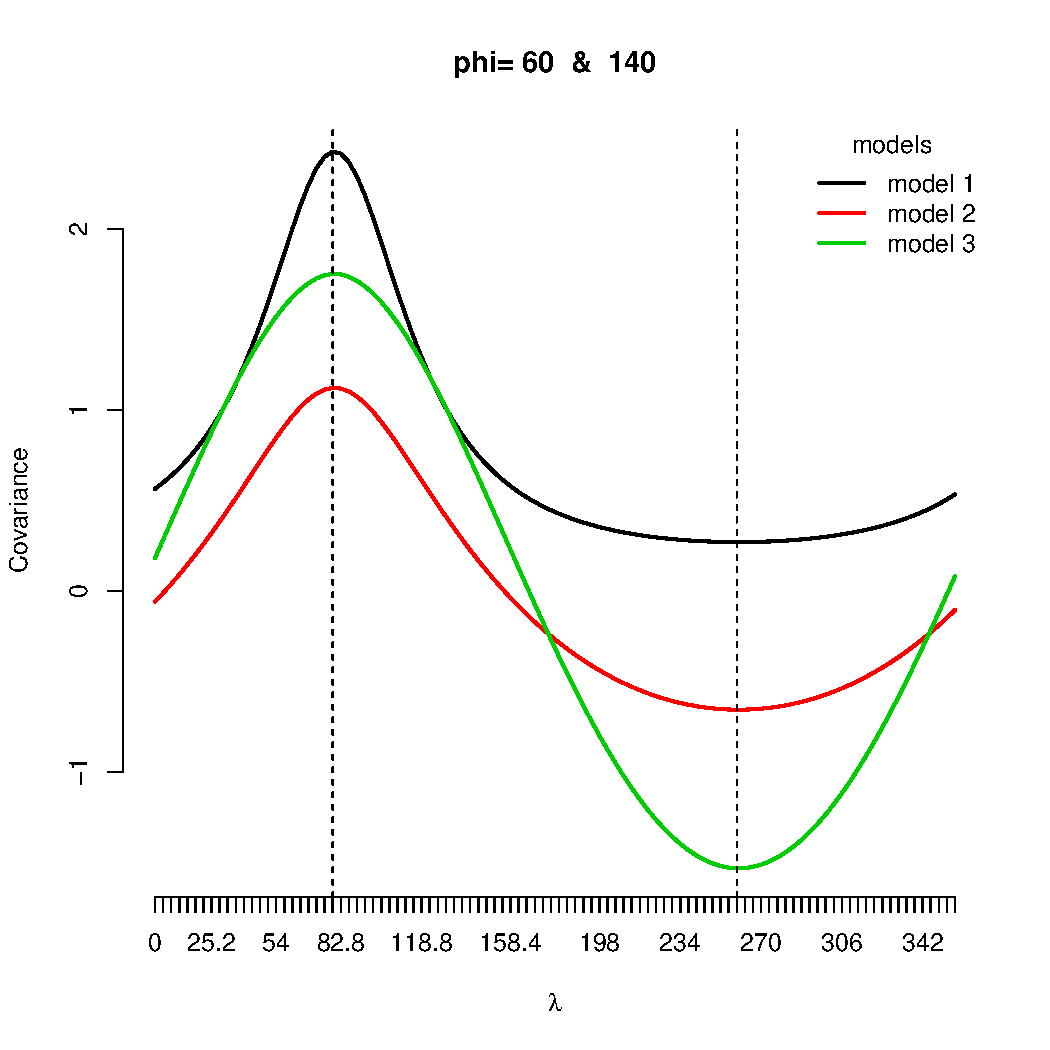
\includegraphics[width=0.7\textwidth]{graphs/all_covariance_models}
				\caption[The Covariance Between $30^0S$ and $50^0N$ (Latitudes $60^0$ and $140^0$) of Three] {The covariance between $30^0S$ and $50^0N$ (latitudes $60^0$ and $140^0$) of three covariance models with exponential family, $ i.e., \tilde{C}(\phi_P, \phi_Q)$ given by \eqref{Cm_model1} over 100 longitudes (we set $C_1 = C_2 = a = u = 1$, and $p = 0.5$).}
			\end{figure}
				
\rmark{The parameters $C_1, C_2, a, p$ are scaling parameters of the covariance functions and $u$ is a location parameter. All covariance models have a similar pattern and share one property. When there is no location shift ($u = 1$), the maximum of $R(P,Q)$ occurs at $\lambda_{max} = |\phi_P -\phi_Q|$ and the minimum of $R(P,Q)$ occurs at $\lambda_{min} = \pi + \lambda_{max}$. } 
					
			\begin{figure}
				\centering
				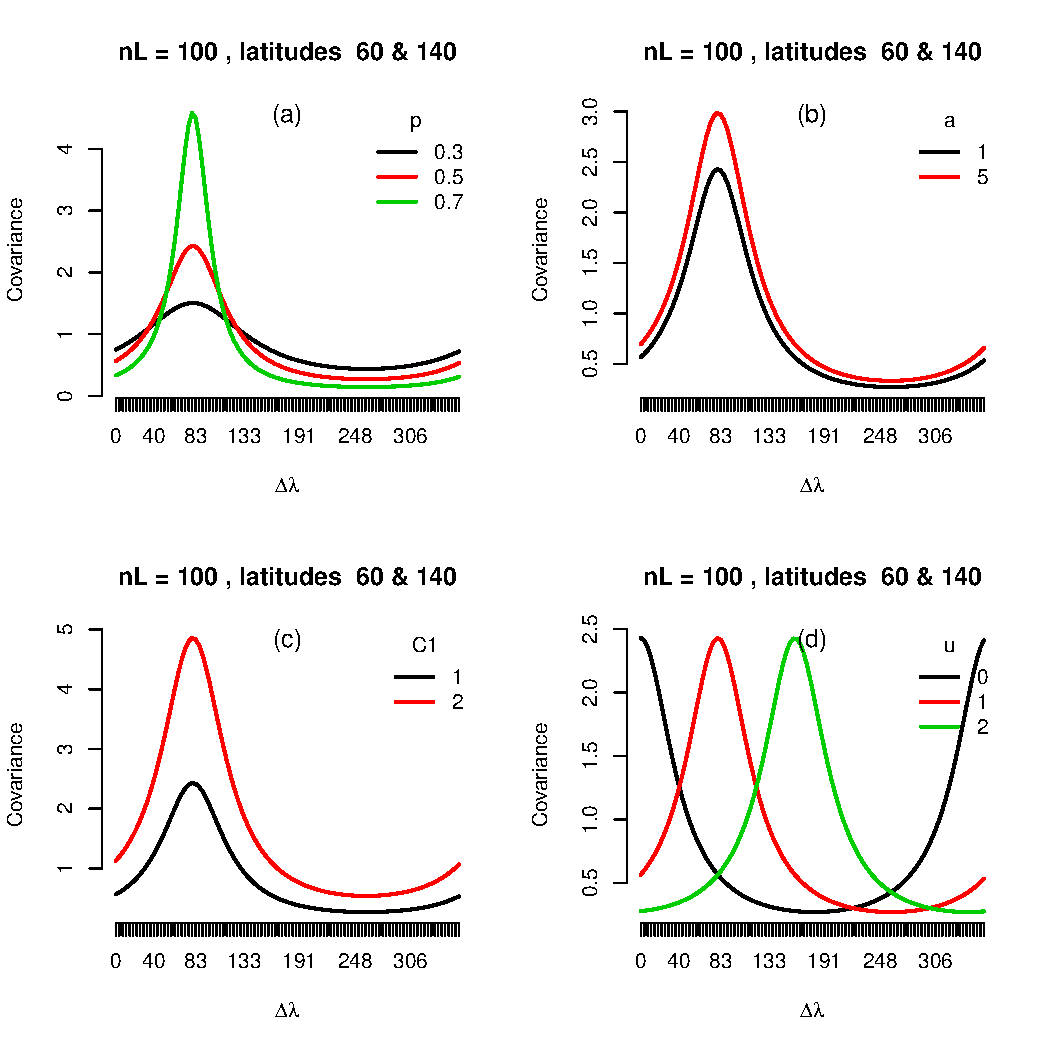
\includegraphics[width=1\textwidth]{graphs/parameters_model1_2}
				\caption[Covariance Curves for Different Parameters using Model1:] {Covariance curves for different parameters using model 1 \citep{Huang2012}:  (a)-parameter $p$, (b)-parameter $a$, (c)-parameter $C_1$ (similar pattern for parameter $C_2$), (d)-parameter $u$}
				\label{fig_parameter_comp}
			\end{figure}
			
\rmark{The scaling parameter $p$ changes rapidly at the supremum and infimum of the covariance models and parameters $C_1, C_2$, and $a$ are regular scaling parameters. The parameter $u$ is a location parameter which shifts the covariance from left to right with respect to $\Delta\lambda$) when $u>0$. When $u=0$ it provides a longitudinally reversible covariance model.}

%%------------------------------------------------------------------%%
\section{Covariance and Variogram Estimators on a Sphere}
%%------------------------------------------------------------------%%
			%In contrast the cross variogram is an even function when the process is intrinsically stationary.

The covariance function $R(P, Q)$ has also be termed as a cross covariance in the literature, as it captures the covariance of the process between points at two latitudes with longitudes separated by $\Delta \lambda \in (-\pi,\pi)$. In this section, we consider the estimator for the covariance function $R(P, Q)$ based on MOM as well as its properties. In addition, we will introduce the cross variogram function on the sphere. The unbiasedness of the cross variogram estimator based on MOM will also be discussed.


%%------------------------------------------------------------------%%
\subsection{Cross Covariance and Cross Variogram Functions}
%%------------------------------------------------------------------%%

As discussed in \cite{Wackernagel2013}, the cross covariance function, or $R(P, Q)$, can be decomposed as the following:
\begin{eqnarray*}
R(\phi_P, \phi_Q, \Delta \lambda) &=& \frac{1}{2}(R(\phi_P, \phi_Q, \Delta \lambda) + R(\phi_P, \phi_Q, -\Delta \lambda)) \\
& & + \frac{1}{2}(R(\phi_P, \phi_Q, \Delta \lambda) - R(\phi_P, \phi_Q, -\Delta \lambda)).
\end{eqnarray*}
For fixed latitudes $\phi_P$ and $\phi_Q$, the first term is an even function of $\Delta \lambda$, while the second term is an odd function of $\Delta \lambda$. We notice that, when $\phi_P \ne \phi_Q$, $R(\phi_P, \phi_Q, \Delta \lambda)$ has the following properties:
\begin{itemize}
\item $R(\phi_P, \phi_Q, \Delta \lambda) \ne R(\phi_Q, \phi_P, \Delta \lambda)$;
\item $R(\phi_P, \phi_Q, -\Delta \lambda) \ne R(\phi_P, \phi_Q, \Delta \lambda)$;
\item $R(\phi_P, \phi_Q, -\Delta \lambda) = R(\phi_Q, \phi_P, \Delta \lambda)$.
\end{itemize}
As a special case, when $\phi_P = \phi_Q$ fixed, two locations are on the same circle, the cross covariance $R(\phi_P, \phi_P, \Delta\lambda)$ is a stationary covariance function on the circle, a function depending on longitudinal difference ($\Delta\lambda$) only. \\

Now we introduce the cross variogram function on the sphere. The cross variogram function is defined as following:
\[
2\gamma(\phi_p, \phi_Q, \Delta\lambda) = E\left((X(\phi_P, \lambda+\Delta \lambda) - X(\phi_P, \lambda))(X(\phi_Q, \lambda+\Delta \lambda) - X(\phi_Q, \lambda))\right).
\]
When $\phi_P = \phi_Q$, the above expression reduces to the expression for the variogram function on the circle.\\
\noi Note that
\begin{eqnarray*}
\gamma(\phi_p, \phi_Q, \Delta\lambda) &=& \frac{1}{2}E\left((X(\phi_P, \lambda+\Delta \lambda) - X(\phi_P, \lambda))(X(\phi_Q, \lambda+\Delta \lambda) - X(\phi_Q, \lambda))\right) \\
&=& \frac{1}{2} E\left(((X(\phi_P, \lambda+\Delta \lambda) - \mu_P) - (X(\phi_P, \lambda)- \mu_P)) \right. \\
& & \left.((X(\phi_Q, \lambda+\Delta \lambda) - \mu_Q) - (X(\phi_Q, \lambda) - \mu_Q)\right) \\
&=& \frac{1}{2} \left(cov(X(\phi_P, \lambda+\Delta \lambda), X(\phi_Q, \lambda+\Delta \lambda)) \right. \\
& &- \left.cov(X(\phi_P, \lambda+\Delta \lambda), X(\phi_Q, \lambda)) \right. \\
& & \left. - cov(X(\phi_P, \lambda), X(\phi_Q, \lambda + \Delta \lambda)) + cov(X(\phi_P, \lambda), X(\phi_Q, \lambda))  \right) \\
&=& \frac{1}{2} \left(R(\phi_P, \phi_Q, 0) - R(\phi_P, \phi_Q, \Delta \lambda) - R(\phi_P, \phi_Q, -\Delta \lambda) + R(\phi_P, \phi_Q, 0)  \right) \\
&=& R(\phi_P, \phi_Q, 0) - \frac{1}{2}(R(\phi_P, \phi_Q, \Delta \lambda) + R(\phi_P, \phi_Q, -\Delta \lambda)).
\end{eqnarray*}
That is, 				
\beq
\gamma(\phi_p, \phi_Q, \Delta\lambda) =  R(\phi_p, \phi_Q, 0) - \frac{1}{2}(R(\phi_P, \phi_Q, \Delta \lambda) + R(\phi_P, \phi_Q, -\Delta \lambda)).
\eeq
We notice that the (semi-)cross variogram relates to only the even term of the cross covariance function. \cite{Wackernagel2013} argues that cross variogram might not be sufficient when there is a delayed affect, which introduces the non-zero value representing from the odd component in the cross \cov decomposition.\\

When the axially symmetric process $X(P)$ is also longitudinally reversible, that is, $R(\phi_P, \phi_Q, -\Delta \lambda) = R(\phi_P, \phi_Q, \Delta \lambda)$, we have
\begin{eqnarray*}
\gamma(\phi_p, \phi_Q, \Delta\lambda) =  R(\phi_p, \phi_Q, 0) - R(\phi_P, \phi_Q, \Delta \lambda),
\end{eqnarray*}
which is the same relationship as the one between the covariance and variogram functions on the circle.


%%------------------------------------------------------------------%%
\subsection{The MOM Cross Covariance and Cross Variogram Estimators}
%%------------------------------------------------------------------%%

We now provide the MOM estimators for the cross covariance $R(\phi_P, \phi_Q, \Delta \lambda)$ and cross semivariogram function $\gamma(\phi_P, \phi_Q, \Delta \lambda)$ of an axially symmetric process on the sphere. First for any two latitudes $\phi_P$ and $\phi_Q$ with $\{\lambda_i, i = 1, 2, \ldots, n\}$ representing the gridded longitudes on each circle (for simplicity, we assume $n = 2N$ is an even number), then the MOM estimator $\hat{R}(\phi_P, \phi_Q, \Delta \lambda)$ is given by
\beq \label{cross_covariance}
\hat{R}(\phi_P, \phi_Q, \Delta \lambda)= \frac{1}{n}\sum_{i = 1}^n (X(\phi_P, \lambda_i + \Delta \lambda) - \bar{X}_P)(X(\phi_Q, \lambda_i) - \bar{X}_Q),
\eeq
where $\Delta \lambda = 0, 2\pi/n, 4\pi/n, \cdots, 2(N-1)\pi/n$, $\bar{X}_P = \frac{1}{n}\sum_{i=1}^n X(\phi_P, \lambda_i)$, and a similar expression for $\bar{X}_Q$. 

Now we show the unbiasedness of the cross \cov estimator.	
\begin{eqnarray*}
				& & E(\hat{R}(\phi_P, \phi_Q, \Delta \lambda)) \\
				&=& \frac{1}{n}\sum_{i = 1}^n E((X(\phi_P, \Lambda_i) - \bar{X}_P)(X(\phi_Q, \lambda_i) - \bar{X}_Q)) \\
				&=& \frac{1}{n}\sum_{i=1}^n cov(X(\phi_P, \Lambda_i), X(\phi_Q, \lambda_i)) - \frac{1}{n}\sum_{i = 1}^n E((X(\phi_P, \Lambda_i) - \mu_P)(\bar{X}_Q - \mu_Q)) \\
				& & -\frac{1}{n}\sum_{i = 1}^n E((X(\phi_Q, \lambda_i) - \mu_Q)(\bar{X}_P - \mu_P)) + \frac{1}{n}\sum_{i = 1}^n E((\bar{X}_P - \mu_P)(\bar{X}_Q - \mu_Q)) \\
				&=& R(\phi_P, \phi_Q, \Delta \lambda) -E((\bar{X}_Q - \mu_Q)(\bar{X}_P - \mu_P)) - E((\bar{X}_P - \mu_P)(\bar{X}_Q - \mu_Q)) \\
				& & + E((\bar{X}_P - \mu_P)(\bar{X}_Q - \mu_Q)) \\
				&=& R(\phi_P, \phi_Q, \Delta \lambda) - cov(\bar{X}_P, \bar{X}_Q).
\end{eqnarray*}
where $\Lambda_i = \lambda_i + \Delta \lambda$ and note that,
\begin{eqnarray*}
				& & cov(\bar{X}_P, \bar{X}_Q) \\
				&=&  \frac{1}{n^2}\sum_{i = 1}^n \sum_{j=1}^n cov(X(\phi_P, \lambda_i), X(\phi_Q, \lambda_j)) \\
				&=& \frac{1}{n^2}\sum_{i = 1}^n \sum_{j=1}^n R(\phi_P, \phi_Q, (i-j)*2\pi/n) \\
				&=& \frac{1}{n^2}\sum_{i = 1}^n \sum_{j=1}^n  C_0(\phi_P, \phi_Q)  + 2\sum_{m=1}^\infty \left( C_{m, R}(\phi_P, \phi_Q) \cos(m*(i-j)*2\pi/n) \right. \\
				& & - \left. C_{m, I}(\phi_P, \phi_Q) \sin(m*(i-j)*2\pi/n) \right) \\
				&=& C_0(\phi_P, \phi_Q) + 2\sum_{m=1}^\infty C_{m, R}(\phi_P, \phi_Q) \left(\frac{1}{n^2}\sum_{i = 1}^n \sum_{j=1}^n \cos(m(i-j)*2\pi/n)\right) \\
				& & - 2\sum_{m=1}^\infty C_{m, I}(\phi_P, \phi_Q) \left(\frac{1}{n^2}\sum_{i = 1}^n \sum_{j=1}^n \sin(m(i-j)*2\pi/n)\right) \\
				&=& C_0(\phi_P, \phi_Q),
			\end{eqnarray*}			
since
			\begin{eqnarray*}
				& & \sum_{i = 1}^n \sum_{j=1}^n \cos(m*(i-j)*2\pi/n) \\
				&=& \sum_{i=1}^n \sum_{j=1}^n \left(\cos(m*i *2\pi/n)\cos(m*j*2\pi/n)\right. \\
				& & - \left.\sin(m*i *2\pi/n)\sin(m*j*2\pi/n) \right)\\
				&=& \left(\sum_{i=1}^n \cos(m*i *2\pi/n)\right)^2 - \left(\sum_{i=1}^n \sin(m*i *2\pi/n)\right)^2 = 0
			\end{eqnarray*}
and
			\begin{eqnarray*}
				& & \sum_{i = 1}^n \sum_{j=1}^n \sin(m*(i-j)*2\pi/n) \\
				&=& \sum_{i=1}^n \sum_{j=1}^n \left(\sin(m*i *2\pi/n)\cos(m*j*2\pi/n)\right. \\
				& & - \left.\cos(m*i *2\pi/n)\sin(m*j*2\pi/n) \right)\\
				&=& \left(\sum_{i=1}^n \cos(m*i *2\pi/n)\right)* \left(\sum_{i=1}^n \sin(m*i *2\pi/n)\right) \\
				& & - \left(\sum_{i=1}^n \cos(m*i *2\pi/n)\right)* \left(\sum_{i=1}^n \sin(m*i *2\pi/n)\right) = 0.
			\end{eqnarray*}
Note for any integer $m$, we have
			\[
				\sum_{k = 1}^{n} \cos(mk*2\pi/n) = \left\{\begin{array}{cc}
				0, & \mbox{for any integer $m \ne 0$,}  \\
				n, & \mbox{for $m = 0$}
				\end{array}
				\right. \mbox{ and }
				\sum_{k = 1}^{n} \sin(mk*2\pi/n) = 0.
			\]
Hence,
			\[
				cov(\bar{X}_P, \bar{X}_Q) = C_0 (\phi_P, \phi_Q).
			\]
Therefore,
			\[
				E(\hat{R}(\phi_P, \phi_Q, \Delta \lambda)) = R(\phi_P, \phi_Q, \Delta \lambda) - C_0 (\phi_P, \phi_Q).
			\]
We summarize the above calculations as the following proposition.
\begin{prop}
The MOM cross covariance estimator is biased with the constant shift given by $C_0(\phi_P, \phi_Q) = cov(\bar{X}_P, \bar{X}_Q)$. Hence, the true $R(P, Q)$ may not be identifiable based on the MOM estimator.  
\end{prop}

\vskip 8pt				
				
\rmark{When $\phi_P = \phi_Q$, the result above reduces to that for the MOM covariance estimator on the circle.}

\vskip 8pt				

\rmark{If the mean at each latitude is zero, then we can rewrite the cross covariance MOM estimator as following:			
			\[
				\hat{R}(\phi_P, \phi_Q, \Delta \lambda)= \frac{1}{n}\sum_{i = 1}^n X(\phi_P, \lambda_i + \Delta \lambda)X(\phi_Q, \lambda_i).
			\]
One can	show that this estimator is unbiased.} 

\vskip 8pt				

Next we consider the MOM cross semivariogram estimator for axially symmetric processes on the sphere.				
			\beq \label{cross_variogram}
			\hat{\gamma}(\phi_p, \phi_Q, \Delta\lambda) = \frac{1}{2n} \sum_{i=1}^n \left(X(\phi_P, \Lambda_i) - X(\phi_P, \lambda_i))(X(\phi_Q, \Lambda_i) - X(\phi_Q, \lambda_i))\right),
			\eeq
where $\Lambda_i = \lambda_i+\Delta \lambda$. We have
			\begin{eqnarray*}
				E(\hat{\gamma}_{PQ}(\Delta \lambda)) &=& \frac{1}{2n} \sum_{i=1}^n E\left(X(\phi_P, \Lambda_i) - X(\phi_P, \lambda_i))(X(\phi_Q, \Lambda_i) - X(\phi_Q, \lambda_i))\right) \\
				&=& \frac{1}{2n} \sum_{i=1}^n \left( 2\gamma(\phi_p, \phi_Q, \Delta\lambda) \right) = \gamma(\phi_p, \phi_Q, \Delta\lambda),
			\end{eqnarray*}
			which is unbiased. Here we summarize our finding as follow.

\pro{
The MOM cross semivariogram estimator is unbiased.
}

\vskip 8pt				
				
\rmark{We expect the similar result as the one in the case of ciccle for the consistency of the MOM cross semivariogram estimator on the sphere, but the proof will be more complicated. This will be one of the areas for our future research.}
				
%\end{document}			
			


%%------------------------------------------------------------------%%
\chapter{Global Data Generation and Estimation on the Sphere}
%\documentclass[12pt, amstex, letterpaper] {report} %{article}


\usepackage[margin=1in]{geometry}
\topmargin -0.5in \textwidth 6.5in \textheight 9in
\footskip .5in
\headheight 0.3in


\usepackage{Sweave}

\DefineVerbatimEnvironment{Sinput}{Verbatim} {xleftmargin=0em,frame=single}
\DefineVerbatimEnvironment{Soutput}{Verbatim} {xleftmargin=0em,frame=single}

\usepackage{amssymb, mathrsfs, amsmath, amsfonts}
\usepackage{enumerate, comment}
\usepackage{hyperref, natbib,apalike, float} %cite
\usepackage{color, multirow, setspace, fancyhdr,graphicx}
\usepackage{undertilde}
\usepackage[bottom]{footmisc}
\usepackage{graphicx}
\usepackage{framed}
\usepackage{subcaption}
\usepackage{amsthm}

%\doublespacing
\pagestyle{empty}
\pagestyle{fancy}
\lhead{ }
%\rhead{May 2016}
\fancyfoot{ }
\rfoot{Dissertation $|$ \thepage}
\lfoot{Chris Vanlangenberg}
\date{}

\includecomment{comment}

\newtheorem{theorem}{Theorem}[section]
\newtheorem{defn}{Definition}[section]
\newtheorem{prop}{Proposition}
\newcommand{\pro}[1]{\begin{prop}{#1}\end{prop}}

%\newtheorem{proof}{proof}
\newtheorem{rmk}{Remark}
\newcommand{\rmark}[1]{\begin{rmk}{#1}\end{rmk}}

\numberwithin{equation}{section}
\renewcommand{\footrulewidth}{0.1pt}
\renewcommand{\headrulewidth}{0.1pt}


\newcommand{\eqn}[1]{\begin{equation}{#1}\end{equation}}

\newcommand{\beq}{\begin{equation}}
\newcommand{\eeq}{\end{equation}}
%\renewcommand\refname{Literature}
\newcommand{\blue}[1]{\textcolor{blue}{\emph{#1}}}
\newcommand{\red}[1]{\textcolor{red}{\emph{#1}}}
\newcommand{\twoc}[2]{{\textcolor{blue}{#1}} and {\textcolor{red}{#2}}}


\newcommand{\xn}{x_1,\ldots, x_n}
\newcommand{\Xn}{X_1,\ldots, X_n}
\newcommand\floor[1]{\lfloor{#1}\rfloor}
\newcommand\ceil[1]{\lceil{#1}\rceil}

\newcommand{\X}{\mathcal{X}}
\newcommand{\Sp}{\mathbb{S}}
\newcommand{\R}{\mathbb{R}}
\newcommand{\C}{\mathbb{C}}
\newcommand{\pd}{positive definite }



\newcommand{\code}[1]{{\small\texttt{#1}}}
\newcommand{\pkg}[1]{{\normalfont\textsf{#1}}}
\newcommand{\var}[1] {{\normalfont\textbf{#1}}}
\newcommand{\Cm}{$C_m(\phi_P, \phi_Q)\ $}

\newcommand{\jun}{\cite{JunStein2008}}
%
%\begin{document}


%%-------------------------Data generation---------------------------------------%%

%==========================
\section{Introduction}
%==========================

Statistical simulations have been one of the critical components in statistical research. Through simulations, the researcher can explore how a proposed statistical model/method behaves in the simulated and reproducible data that mimic the real applications. For axially symmetric data generation, there seems only a limited research in literature. In order to capture non-stationarity, \cite{JunStein2007} proposed spatio-tempo covariance functions on the sphere by applying first order differential operator to fully symmetric spatio-tempo processes on sphere. Further, \cite{JunStein2008} extended the above approach and used the Discrete Fourier Transform (DFT) to find out the inverse of the covariance matrix when calculating the exact likelihood for the data on regular grids. They indicated that the inverse of the covariance matrix for axially symmetric data is of the order of $O(n_l^3 n_L)$ where $n_L$ is the number of longitudes and $n_l$ the number of latitudes. However, no data generation and simulation was discussed. \cite{Li2013} proposed convolution methods to generate random fields with a class of Mat\'{e}rn-type kernel functions by allowing the parameters in the kernel function to vary with latitudes. They conducted a simulation study by generating data based on their proposed method. They used maximum likelihood estimation and local smoothing to recover the given parameters. In the recent work by \cite{JeongJun2015}, they presented a number of simulation scenarios using the Mat\'{e}rn-like covariance models that include stationary and non-stationary processes. They seemed to generate data for simulations based in the given \cov structure directly. No data validation was given. As we have discussed in the previous chapters, the global data normally exhibit both complexity and high dimensionality. For example, the MSU data was observed on a $72 \times 144$ grid which results in an estimated covariance matrix with a dimension of $10368\times 10368$. Hence, it is necessary to develop an algorithm that is efficient and with low dimensionality. In this research, we use the Discrete Fourier Transform to decompose the process as Fourier series on the circles, and represent the random Fourier coefficients with circularly-symmetric complex random vectors. This has greatly reduced both computational cost as well as dimensionality. It also gives a better insight about the axially symmetric process on the sphere.\\

This chapter is organized as follow. We first layout the details and methodologies of generating data on a sphere using circularly-symmetric random vectors. Then we provide an algorithm for global data generation process. Finally, we conduct simulations and use the cross variogram and cross \cov MOM estimation to validate the data generated.
		
	%%------------------------------------------------------------------%%
	\section{Method Development}
	%%------------------------------------------------------------------%%

Let $X(P)$ be a continuous real-valued Gaussian random process defined on a unit sphere $\Sp^2$, where $P = (\lambda, \phi) \in \Sp^2$ with longitude $\lambda \in [-\pi, \pi)$ and latitude $\phi \in [0, \pi]$. Following Remark 2.5 in \cite{Huang2012}, for each fixed latitude $\phi$, $X(P)$ can then be represented as a stationary process on the circle. More specifically,			
	\beq \label{eq:sym_process}
	X(\phi, \lambda) = \sum_{m=-\infty}^{\infty} W_m(\phi) e^{i m \lambda},
	\eeq
where
\[	
W_m(\phi) = \frac{1}{2\pi} \int_0^{2\pi} X(\phi, \lambda) e^{-i m \lambda} d \lambda,
\]
with $\mbox{E}(W_m(\phi_P) \overline{W_n(\phi_Q)}) = \delta{(m,n)} C_m(\phi_P, \phi_Q)$. That is, $\{W_m(\phi), \phi \in [0,\pi], m = 0, \pm 1, \pm 2, \ldots,\}$ are uncorrelated Gaussian complex random variables with covariance function given by $C_m(\phi_P, \phi_Q)$.\\		
			
In order to obtain axially symmetric random variates for a given latitude $\phi$, we first construct normal independent (complex) random variates $W_m(\phi)$ that follow the given  variance-covariance function $C_m(\phi_P, \phi_Q)$. To achieve this, we truncate the infinite summation in (\ref{eq:sym_process}) to obtain a finite summation up to $N$ as given below (with the abuse of notation $X(P)$ for notation simplicity).
	\beq
	X(P) = X(\phi, \lambda) = \sum_{m=-N}^{N} W_m(\phi) e^{i m \lambda}.
	\eeq
Since $W_m$'s are independent for $m =0, \pm 1, \pm 2, \cdots, \pm N$, we have			
	\begin{eqnarray*}
		Cov(X(P), {X(Q)}) &=& Cov\left(\sum_{m = -N}^{N} W_m(\phi_P) e^{i m \lambda_P}, \sum_{j=-N}^{N} {W_j(\phi_Q)} e^{i j \lambda_Q}\right) \\
		&=& \sum_{m, j} e^{i m \lambda_P} e^{-i j \lambda_Q} Cov(W_m(\phi_P), {W_j(\phi_Q)}) \\
		&=& \sum_{m} e^{im (\lambda_P - \lambda_Q)} C_m(\phi_P, \phi_Q),
	\end{eqnarray*}
indicating that the Fourier series for covariance function $R(P, Q)$ has also been truncated up to $N$. Let $W_m(\phi) = W_{m}^{r}(\phi) + i W_{m}^i(\phi)$ and $C_m(\phi_P, \phi_Q) = C_m^r(\phi_P, \phi_Q) + i C_m^i(\phi_P, \phi_Q)$. \\

In order to obtain real data values that follow the given $R(P, Q)$, we require that
\begin{itemize}
\item $W_{-m}(\phi) = \overline{W_m(\phi)}$, and
\item $ C_{-m} (\phi_P, \phi_Q) = \overline{C_m(\phi_P, \phi_Q)}, \quad \mbox{for $m = 0, 1, 2, \cdots, N$.}$
% \label{eq:for_real}
\end{itemize}
First we simplify the process.
	\begin{eqnarray} \label{eq:finite_process}
		X(P) &=& \sum_{m = -N}^N W_m(\phi) e^{im \lambda} =  W_0(\phi) + \sum_{m =1}^N W_m(\phi) e^{im \lambda} + \sum_{m =-1}^{-N} W_m(\phi) e^{im \lambda} \nonumber \\
		&=& W_0(\phi) + \sum_{m =1}^N W_m(\phi) e^{im \lambda} + \sum_{m =1}^{N} \overline{W_m(\phi)} e^{-im \lambda} \nonumber \\
		&=& W_0(\phi) + \sum_{m =1}^N \left[  (W_m^r(\phi)+iW_m^i(\phi))(\cos(m \lambda) + i \sin(m \lambda)) \right. \nonumber \\
		& & \left. +\ (W_m^r(\phi)-iW_m^i(\phi))(\cos(m \lambda) - i \sin(m \lambda))  \right]  \nonumber \\
		&=& W_0(\phi) + 2 \sum_{m =1}^N \left[W_m^r(\phi)\cos(m\lambda) - W_m^i(\phi)\sin(m \lambda)\right].
	\end{eqnarray}
Now we consider the corresponding variance-covariance function for each $W_m(\phi)$.  \\ 			
 
Note that to have the real-valued data observations, hence
	\beq \label{eq:for_real}
	C_{-m} (\phi_P, \phi_Q) = \overline{C_m(\phi_P, \phi_Q)}, \quad \mbox{for $m = 1, 2, \cdots, N$}.
	\eeq
	Writing \Cm = $C_m^{r}(\phi_P, \phi_Q) + iC_m^{i}(\phi_P, \phi_Q)$ and with \eqref{eq:for_real}, we have
	% Le $W_m(\phi) = W_{m}^{r}(\phi) + i W_{m}^i(\phi)$ in terms of a real component and an imaginary component. We also write 
	% and with the relationship \ref{eq:for_real} above, 
	\[
		C_{-m}^r(\phi_P, \phi_Q) = C_{-m}^r(\phi_P, \phi_Q), \quad C_{-m}^i(\phi_P, \phi_Q) = - C_{-m}^i(\phi_P, \phi_Q).
	\]
	Now,
	\begin{eqnarray*}
		Cov(W_m(\phi_P), {W_m(\phi_Q)}) &=& Cov(W_m^r(\phi_P) + iW_m^i(\phi_P), W_m^r(\phi_Q) + i W_m^i(\phi_Q)) \\
		&=& \left[Cov(W_m^r(\phi_P), W_m^r(\phi_Q)) + Cov(W_m^i(\phi_P), W_m^i(\phi_Q))\right] \\
		& & + i\left[- Cov(W_m^r(\phi_P), W_m^i(\phi_Q)) + Cov(W_m^i(\phi_P), W_m^r(\phi_Q))\right] \\
		&=& C_m^r(\phi_P, \phi_Q) + i C_m^i(\phi_P, \phi_Q).
	\end{eqnarray*}
	In addition, we set the following.		
	\begin{eqnarray} \label{real_cov}
		& & Cov(W_m^r(\phi_P), W_m^r(\phi_Q)) = Cov(W_m^i(\phi_P), W_m^i(\phi_Q)) = \frac{1}{2}C_m^r(\phi_P, \phi_Q), \label{real_cov} \\
		& & Cov(W_m^i(\phi_P), W_m^r(\phi_Q)) = - Cov(W_m^r(\phi_P), W_m^i(\phi_Q)) = \frac{1}{2}C_m^i(\phi_P, \phi_Q). \label{im_cov}
	\end{eqnarray}
The above relationships \eqref{real_cov} and \eqref{im_cov} will become our basis for data generation.
	
	
	%-------------------------------------%
	\subsection{Data Generation}
	%-------------------------------------%
	
Now for each fixed $m = 0, 1, 2, \cdots, N$, we write  $W_m(\phi) = W_m^r(\phi) + i W_m^i(\phi)$ then $\overline{W_m}(\phi) = W_m^r(\phi) - i W_m^i(\phi)$. We may assume that $W_m^r(\phi)$ and $W_m^i(\phi)$ are independent, each following a (Gaussian) distribution with mean zero and the same variance $\sigma_m^2(\phi) = \frac{1}{2}C_m^r(\phi, \phi)$ and $C_m^i(\phi, \phi) = 0$ (that is, $W_m(\phi)$ is circularly symmetric). For a set of distinct latitudes $\Phi = \{\phi_1, \phi_2, \cdots, \phi_{n_l}\}$, we consider a sequence of complex random variables $\{W_m(\phi): \phi \in \Phi\}$, which forms a multivariate complex random vector $\utilde{W}_m = (W_m(\phi_1), W_m(\phi_2), \cdots, W_m(\phi_n))^T$ where $W_m(\phi_i) = W_m^r(\phi_i) + iW_m^r(\phi_i)$ with associated $2\times n_l$-dimensional real random vector
\begin{eqnarray*}
		\utilde{V}_m  &=& (W_m^r(\phi_1),\cdots,W_m^r(\phi_{n_l}), W_m^i(\phi_1), \cdots, W_m^i(\phi_{n_l}))^T \\
		&=& (Re(\utilde{W}_m), Im(\utilde{W}_m))^T.
	\end{eqnarray*}

% Following the definition for a complex circularly-symmetry random vector introduced in Chapter 1, 

We now show that the Gaussian random vector $\utilde{W}_m$ is circularly-symmetric, that is, we calculate the covariance matrix $K_W = E(\utilde{W}_m\utilde{W}_m^*)$ (where $\utilde{W}_m^*$ is the conjugated transpose of $\utilde{W}_m$) and pseudo-covariance $M_W = E(\utilde{W}_m\utilde{W}_m^T)$, and show that $M_W=0$. First note that 
	\begin{eqnarray*}
		M_W & = & \left(\begin{array}{cccc}
		E[W_m(\phi_1) W_m(\phi_1) ] & E[W_m(\phi_1) W_m(\phi_2) ]  & \cdots & E[W_m(\phi_1) W_m(\phi_{n_l}) ]\\
		E[W_m(\phi_2) W_m(\phi_1) ] & E[W_m(\phi_2) W_m(\phi_2) ]  & \cdots & E[W_m(\phi_2) W_m(\phi_{n_l}) ]\\
		\vdots & \vdots  & \ddots & \vdots \\
		E[W_m(\phi_{n_l}) W_m(\phi_1) ] & E[W_m(\phi_{n_l}) W_m(\phi_2) ]  & \cdots & E[W_m(\phi_{n_l}) W_m(\phi_{n_l})]
		\end{array}
		\right).
	\end{eqnarray*}
We calculate each of the above entries.	For any $i,j$,
	\begin{eqnarray*}
		& & E[W_m(\phi_i) W_m(\phi_j) ]\\
		&=& E[(W_m^r(\phi_i) + i W_m^i(\phi_i))(W_m^r(\phi_j) + i W_m^i(\phi_j))] \\
		&=& E(W_m^r(\phi_i)W_m^r(\phi_j)) - E(W_m^i(\phi_i)W_m^i(\phi_j)) \\
		& & + i[E(W_m^r(\phi_i)W_m^i(\phi_j)) + E(W_m^i(\phi_i)W_m^r(\phi_j))] \\
		&=& \left\{\begin{array}{ll}
        \frac{1}{2}(C_m^r(\phi_i, \phi_j) - C_m^r(\phi_i, \phi_j)) + i [-\frac{1}{2} C_m^i(\phi_i, \phi_j) + \frac{1}{2}C_m^i(\phi_i, \phi_j)] = 0 & \mbox{for $i \ne j$} \\
		\frac{1}{2}(C_m^r(\phi_i, \phi_i) - C_m^r(\phi_i, \phi_i)) + i [0 + 0] = 0 &  \mbox{for $i = j$}.
\end{array}
\right.
	\end{eqnarray*}
The last equality is due to the independence of $W_m^r(\phi_i)$ and $W_m^i(\phi_i)$. Therefore, $M_W = 0$, and so $\utilde{W}_m$ is circularly-symmetric. In addition,
	\begin{eqnarray*}
		K_W & = & E(\utilde{W}_m\utilde{W}_m^*) \\
		& = &\left(\begin{array}{cccc}
		E[W_m(\phi_1) W_m^*(\phi_1) ] & E[W_m(\phi_1) W_m^*(\phi_2) ]  & \cdots & E[W_m(\phi_1) W_m^*(\phi_{n_l}) ]\\
		E[W_m(\phi_2) W_m^*(\phi_1) ] & E[W_m(\phi_2) W_m^*(\phi_2) ]  & \cdots & E[W_m(\phi_2) W_m^*(\phi_{n_l}) ]\\
		\vdots & \vdots  & \ddots & \vdots \\
		E[W_m(\phi_{n_l}) W_m^*(\phi_1) ] & E[W_m(\phi_{n_l}) W_m^*(\phi_2) ]  & \cdots & E[W_m(\phi_{n_l}) W_m^*(\phi_{n_l})]
		\end{array}
		\right)\\
		& = &\left(\begin{array}{cccc}
		C_{11}^r & C_{12}^r+iC_{12}^i & \cdots & C_{1n_l}^r+iC_{1n_l}^i\\
		C_{21}^r-iC_{21}^i & C_{22}^r & \cdots & C_{2n_l}^r+iC_{2n_l}^i\\
		\vdots & \vdots  & \ddots & \vdots \\
		C_{n_l1}^r-iC_{n_l1}^i & C_{n_l2}^r-iC_{n_l2}^i & \cdots & C_{n_ln_l}^r\\
		\end{array}
		\right) \\
		& = &\left(\begin{array}{cccc}
		C_{11}^r & C_{12}^r & \cdots & C_{1n_l}^r\\
		C_{21}^r & C_{22}^r & \cdots & C_{2n_l}^r\\
		\vdots & \vdots  & \ddots & \vdots \\
		C_{n_l1}^r & C_{n_l2}^r & \cdots & C_{n_ln_l}^r\\
		\end{array}
		\right) + i
		\left(\begin{array}{cccc}
		0 & C_{12}^i & \cdots & C_{1n_l}^i\\
		-C_{21}^i & 0 & \cdots & C_{2n_l}^i\\
		\vdots & \vdots  & \ddots & \vdots \\
		-C_{n_l1}^i & -C_{n_l2}^i & \cdots &  0\\
		\end{array}
		\right)\\
		&=& Re(K_W) + iIm(K_W), 
	\end{eqnarray*}
where $C_m^r(\phi_i, \phi_j) \overset{\bigtriangleup}{=}  C_{ij}^r$ and $C_m^i(\phi_i, \phi_j) \overset{\bigtriangleup}{=}  C_{ij}^i$. Now,
	\begin{eqnarray*}
		K_V & = & E(\utilde{V}_m\utilde{V}_m^*) = E(\utilde{V}_m\utilde{V}_m^T) \\
		&=& \left(\begin{array}{ll}
		E[Re(\utilde{W}_m)Re(\utilde{W}_m)^T] &  E[Re(\utilde{W}_m)Im(\utilde{W}_m)^T] \\
		E[Im(\utilde{W}_m)Re(\utilde{W}_m)^T] &  E[Im(\utilde{W}_m)Im(\utilde{W}_m)^T]
		\end{array}
		\right)_{2n_{l}\times 2n_{l} }.
	\end{eqnarray*}			
Since $\utilde{W}_m$ is circularly-symmetric from \eqref{comlex_cov} we can get the following results,
\begin{eqnarray*}		
E[Re(\utilde{W}_m)Re(\utilde{W}_m)^T] &=& E[Im(\utilde{W}_m)Im(\utilde{W}_m)^T] = \frac{1}{2}(Re(K_W))_{n_{l}\times n_{l}}, \\
E[Re(\utilde{W}_m)Im(\utilde{W}_m)^T] &=& -E[Im(\utilde{W}_m)Re(\utilde{W}_m)^T] = \frac{1}{2}(Im(K_W))_{n_{l}\times n_{l}}.
\end{eqnarray*}
We arrive			
	\begin{eqnarray*}
		K_V&=& \frac{1}{2}\left( \begin{array}{ll}
		Re(K_W) & Im(K_W)^T \\
		Im(K_W) & Re(K_W)
		\end{array}
		\right) = \frac{1}{2}\left( \begin{array}{ll}
		Re(K_W) & -Im(K_W) \\
		Im(K_W) & Re(K_W)
		\end{array}
		\right)
	\end{eqnarray*}
Note that $K_V$ is a non-negative definite matrix, its singular decomposition is given as follows.
	\[ 
	K_V = P\Lambda P^T, 
	\]
where $\Lambda$ is a diagonal matrix with eigenvalues (real-positive) of $K_V$ and $P$ is an orthonormal matrix, containing the corresponding orthonormalized eigenvectors of $K_V$. Let $A = K_V^{1/2} = P\Lambda^{1/2} P^T$ and let $\utilde{Z} =\{z_1^{(1)}, z_2^{(1)}, \ldots, z_{n_l}^{(1)}, z_1^{(2)}, z_2^{(2)}, \ldots, z_{n_l}^{(2)}\}$ be a vector of {\em i.i.d.} standard normal random variates, we obtain 
	\[\utilde{V}_m=A_{2n_{l}\times 2n_{l}}\utilde{Z}_{2n_{l}\times 1},\]
and hence $\utilde{W}_m$.\\

Now for each latitude $\phi_l, l = 1, 2, \cdots, n_l$ and $\lambda_k, k = 1, 2, \cdots, n_L$, we denote the axially symmetric real data as $\{X(\phi_l, \lambda_k)\}$. These random variates can be obtained from the equation (\ref{eq:finite_process}), which is rewritten as below.
	\begin{eqnarray} \label{eq:finite_process_2}
		X(\phi_l,\lambda_k) &=& W_0(\phi_l) + 2 \sum_{m =1}^N \left[W_m^r(\phi_l)\cos(m\lambda_k) - W_m^i(\phi_l)\sin(m \lambda_k)\right].
	\end{eqnarray}
		
	\rmark{For the above decomposition, one needs to compute the eigenvalues and eigenvectors of $K_V$, which has the computational cost of $O((n_l)^2)$.}
	
	%-------------------------------------%
	%\subsection{\bf Pseudo-code}
	%-------------------------------------%
	%   \begin{algorithm}[Pseudo-code] \label{pseudo_code} \hfill
	% 	\begin{itemize}
	% 		  \begin{framed}
	% 		\item Choose a cross covariance function, $R(P,Q)$
	% 		\item Initialize the parameters ($C_1, C_2, a, u, p$) and choose a resolution $\phi_1,\ldots,\phi_{n_l}, \lambda_1, \ldots, \lambda_{n_L}$ (or $n_l\times n_L$),
	% 		\item Derive \Cm based on $R(P,Q)$ where $m=0,1,\ldots,n_L/2$,
	% 		      \begin{enumerate}
	% 		      	\item for each $m$ get $Re(K_W)$ and $Im(K_W)$ hence obtain $K_V$
	% 		      	\item use SVD to get $\utilde{V}_m$ ($n_l-tuples$)
	% 		      	\item get $\utilde{W}_m$'s from $\utilde{V}_m$
	% 		      \end{enumerate}
	% 		      		      		
	% 		\item Apply the equation (\ref{eq:finite_process_2}) to obtain gridded data.
	% 		\end{framed}
	% 	\end{itemize}
	% \end{algorithm}
	
  \begin{algorithm}[Pseudo-code] \label{pseudo_code} \hfill
			\begin{itemize}
			  \begin{framed}
			\item Given a cross covariance function $R(P,Q)$ with given parameters ($C_1, C_2, a, u, p$)
			\item Choose a resolution $\phi_1,\ldots,\phi_{n_l}, \lambda_1, \ldots, \lambda_{n_L}$ (or $n_l\times n_L$)
			\item Obtain \{$W_m$\},
			      \begin{enumerate}
					\item derive \Cm $m=0,1,\ldots,n_L/2$ based on $R(P,Q)$
			      	\item for each $m$ get $Re(K_W)$ and $Im(K_W)$ hence obtain $K_V$
			      	\item use SVD to compute $\utilde{V}_m$ ($n_l-tuples$)
			      	\item get $\utilde{W}_m$'s from $\utilde{V}_m$
			      \end{enumerate}		      		      		
			\item Apply the equation (\ref{eq:finite_process_2}) to obtain gridded data.
			\end{framed}
		\end{itemize}
		\end{algorithm}
	
	%-------------------------------------%
	\section{Simulation Setup}
	%-------------------------------------%
We now implement the algorithm above to obtain axially symmetric data with the given covariance structure. We will use models (\ref{model4}), (\ref{model5}), and (\ref{model6}) discussed in Section 4.3 in the simulation. We select two sets of parameters, which are given below.
\begin{table}[H]
\centering
\caption[Parameter Values]{Parameter values }
\vskip 16pt
\begin{tabular}{|l|l|}
 \hline
 & Parameter values\\ \hline
set 1 : & $C_1 = 1, C_2 = 1, a = 1, u = 1$, $p=0.5$ \\
set 2 : & $C_1 = 1, C_2 = 2, a = 3, u = 1$, $p=0.6$ \\ \hline
\end{tabular}
\end{table}
The parameter $u$ is the location parameter and $u=0$ gives the covariance function of a longitudinally reversible process on a sphere. 

	%-------------------------------------%
	\subsection{Deriving $\mathbf{C_m}$ for Model 1}
	%-------------------------------------%	
%%%%%%%% this is the Appendix A n in data generation paper
%%%%%%%% details of deriving C_m

%\documentclass[12pt, amstex, letterpaper] {report} %{article}


\usepackage[margin=1in]{geometry}
\topmargin -0.5in \textwidth 6.5in \textheight 9in
\footskip .5in
\headheight 0.3in


\usepackage{Sweave}

\DefineVerbatimEnvironment{Sinput}{Verbatim} {xleftmargin=0em,frame=single}
\DefineVerbatimEnvironment{Soutput}{Verbatim} {xleftmargin=0em,frame=single}

\usepackage{amssymb, mathrsfs, amsmath, amsfonts}
\usepackage{enumerate, comment}
\usepackage{hyperref, natbib,apalike, float} %cite
\usepackage{color, multirow, setspace, fancyhdr,graphicx}
\usepackage{undertilde}
\usepackage[bottom]{footmisc}
\usepackage{graphicx}
\usepackage{framed}
\usepackage{subcaption}
\usepackage{amsthm}

%\doublespacing
\pagestyle{empty}
\pagestyle{fancy}
\lhead{ }
%\rhead{May 2016}
\fancyfoot{ }
\rfoot{Dissertation $|$ \thepage}
\lfoot{Chris Vanlangenberg}
\date{}

\includecomment{comment}

\newtheorem{theorem}{Theorem}[section]
\newtheorem{defn}{Definition}[section]
\newtheorem{prop}{Proposition}
\newcommand{\pro}[1]{\begin{prop}{#1}\end{prop}}

%\newtheorem{proof}{proof}
\newtheorem{rmk}{Remark}
\newcommand{\rmark}[1]{\begin{rmk}{#1}\end{rmk}}

\numberwithin{equation}{section}
\renewcommand{\footrulewidth}{0.1pt}
\renewcommand{\headrulewidth}{0.1pt}


\newcommand{\eqn}[1]{\begin{equation}{#1}\end{equation}}

\newcommand{\beq}{\begin{equation}}
\newcommand{\eeq}{\end{equation}}
%\renewcommand\refname{Literature}
\newcommand{\blue}[1]{\textcolor{blue}{\emph{#1}}}
\newcommand{\red}[1]{\textcolor{red}{\emph{#1}}}
\newcommand{\twoc}[2]{{\textcolor{blue}{#1}} and {\textcolor{red}{#2}}}


\newcommand{\xn}{x_1,\ldots, x_n}
\newcommand{\Xn}{X_1,\ldots, X_n}
\newcommand\floor[1]{\lfloor{#1}\rfloor}
\newcommand\ceil[1]{\lceil{#1}\rceil}

\newcommand{\X}{\mathcal{X}}
\newcommand{\Sp}{\mathbb{S}}
\newcommand{\R}{\mathbb{R}}
\newcommand{\C}{\mathbb{C}}
\newcommand{\pd}{positive definite }



\newcommand{\code}[1]{{\small\texttt{#1}}}
\newcommand{\pkg}[1]{{\normalfont\textsf{#1}}}
\newcommand{\var}[1] {{\normalfont\textbf{#1}}}
\newcommand{\Cm}{$C_m(\phi_P, \phi_Q)\ $}

\newcommand{\jun}{\cite{JunStein2008}}
%\begin{document}

As we note that it is very crucial to derive \Cm based on the given $R(P,Q)$. Here is the detailed steps to derive \Cm from model 1 (\ref{model4}). \Cm for other models can be obtained similarly. 
\begin{eqnarray*}
	R(P, Q) &=& R(\phi_P, \phi_Q, \Delta \lambda) = \tilde{C}(\phi_P, \phi_Q) \frac{1-p^2}{1 - 2p \cos(\Theta)+p^2},
\end{eqnarray*}
where $\Theta = \Delta \lambda + u(\phi_P - \phi_Q),$ with some choice of $C_1, C_2, a, u,$ and $p$.

Now,
\begin{eqnarray*}
	C_m(\phi_P, \phi_Q) &=& \frac{1}{2\pi} \int_{-\pi}^\pi R(\phi_P, \phi_Q, \Delta \lambda) e^{-im\Delta \lambda}d\Delta \lambda \\
	&=& \tilde{C}(\phi_P, \phi_Q) \frac{1}{2\pi}\int_{-\pi}^\pi \frac{1-p^2}{1 - 2p \cos(\Theta+p^2} e^{-im\Delta \lambda}d\Delta \lambda.
\end{eqnarray*}

Next we focus on the following integration.
\begin{eqnarray*}
	\int_{-\pi}^\pi \frac{1-p^2}{1 - 2p \cos(x+b)+p^2} e^{-imx}dx,
\end{eqnarray*}
where we set $x=\Delta\lambda$ and $b=u(\phi_P -\phi_Q)$ and we have,
\begin{eqnarray*}
	\frac{1-p^2}{1 - 2p \cos(x+b)+p^2} &=& \frac{2-2p\cos(x+b)-(1-2p \cos(x+b)+p^2)}{1-2p \cos(x+b)+p^2}\\
	&=& 2\times \frac{1-p\cos(x+b)}{1-2p \cos(x+b)+p^2}-1 \\
	&=& 2\times \sum_{n=0}^{\infty}p^n\cos n(x+b)-1  \\
	&=& 1 + 2 \sum_{n=1}^{\infty}p^n (\cos nx \cos(nb) - \sin(nx) \sin(nb)).
\end{eqnarray*}
Therefore, for $m \ne 0$,
\begin{eqnarray*}
	& & \int_{-\pi}^\pi \frac{1-p^2}{1 - 2p \cos(x+b)+p^2} e^{-imx}dx \\
	&=& \int_{-\pi}^\pi \left[1 + 2 \sum_{n=1}^{\infty}p^n (\cos nx \cos(nb) - \sin(nx) \sin(nb))\right]  e^{-imx}dx \\
	&=& \int_{-\pi}^\pi e^{-imx}dx + 2 \sum_{n=1}^{\infty}p^n \int_{-\pi}^\pi \left[\cos nx \cos(nb) - \sin(nx) \sin(nb)\right]  e^{-imx}dx \\
	&=& 2 \sum_{n=1}^{\infty}p^n \left[\cos(nb)  \int_{-\pi}^\pi \cos(nx) e^{-imx} dx - \sin(nb)  \int_{-\pi}^\pi \sin(nx) e^{-imx}dx \right] \\
	&=& 2 \sum_{n=1}^{\infty}p^n \left[ \pi \cos(nb) \delta(n, m) + \pi i\sin(nb)\right] \\
	&=& 2\pi p^m e^{imb}.
\end{eqnarray*}
That is, for $m \ne 0$,
\begin{eqnarray*}
	C_m(\phi_P, \phi_Q)  &=& \tilde{C}(\phi_P, \phi_Q) \frac{1}{2\pi} (2\pi p^m e^{imb}) \\
	&=& \tilde{C}(\phi_P, \phi_Q) p^m e^{imb},
\end{eqnarray*}
and for $m = 0$, $C_0(\phi_P, \phi_Q) = \tilde{C}(\phi_P, \phi_Q)$.\\

In summary,
\begin{eqnarray*}
	C_m(\phi_P, \phi_Q) &=& \left\{ \begin{array}{ll}
	\tilde{C}(\phi_P, \phi_Q), & m = 0 \\
	\tilde{C}(\phi_P, \phi_Q)p^m e^{imb}, & m \ne 0.
	\end{array}
	\right.
	%&=& C_1\left(C_2 - e^{-a|\phi_P|} - e^{-a|\phi_Q|} + e^{-a|\phi_P - \phi_Q|}\right)p^m (\cos(mu(\phi_P - \phi_Q))+i \sin(mu(\phi_P - \phi_Q))).
\end{eqnarray*}

% If the process is longitudinally reversible one can set $u=0$. Suppose 
 
If $\tilde{C}(\phi_P, \phi_Q)$ is  given by \eqref{Cm_model1} then \Cm for model 1 is given by,
\begin{eqnarray*}
	C_m(\phi_P, \phi_Q) &=& \left\{ \begin{array}{ll}
	C_1\left(C_2 - e^{-a|\phi_P|} - e^{-a|\phi_Q|} + e^{-a|\phi_P - \phi_Q|}\right)     & m = 0 \\
	C_1\left(C_2 - e^{-a|\phi_P|} - e^{-a|\phi_Q|} + e^{-a|\phi_P - \phi_Q|}\right)p^m  & m \ne 0.
	\end{array}
	\right.
\end{eqnarray*}




%\end{document}
	

The \Cm functions for all three proposed models are given below,
				\begin{table}[H]
				\centering
				\caption[The $C_m(\cdot, \cdot)$ Functions for Covariance Models used in Data Generation]{The $C_m(\cdot, \cdot)$ functions for covariance models used in data generation}
				\label{Cm_table}
			  \vskip 16pt
				\begin{tabular}{|l|l|l|}
					\hline
					Model   & $C_m(\phi_P, \phi_Q)$                                         & Parameters                               \\
					\hline \hline
					model 1 & $\tilde{C}(\phi_P, \phi_Q) p^m  \mbox{ and } C_0 = \tilde{C}(\phi_P, \phi_Q)$          & $m=0, \pm 1, \pm 2,... \quad p\in (0,1)$ \\
					model 2 & $\tilde{C}(\phi_P, \phi_Q) \frac{p^m}{m} \mbox{ and } C_0 = 0$ & $m=\pm 1, \pm 2,... \quad p\in (0,1)$    \\
					model 3 & $\tilde{C}(\phi_P, \phi_Q) \frac{1}{m^4} \mbox{ and } C_0 = 0$  & $m=\pm 1, \pm 2,...$                     \\
					\hline
				\end{tabular}
			\end{table}

\noi Note that out of above three models, model 1 has $C_0(\phi_P, \phi_Q) \ne 0$. Hence, from Chapter 4, the MOM cross covariance estimator is biased with the non-estimable shift. On the other hand, both models 2 and 3 have $C_0 = 0$, and hence one could use the unbiased MOM cross covariance estimator for data validation. 

%==============================================
\subsection{Data Generation Through R(P, Q)}
%==============================================

In order to demonstrate how effective our data generation algorithm is, we also consider the data generated through the given covariance matrix $R(P, Q)$ directly. Note that the covariance matrix $R(P, Q)$ is a real block circulant matix with the following (\citealp{Li2013, JunStein2008}). 
 \begin{eqnarray}
	R(P,Q) &=& \left[
		\begin{array}{lllll}
			R_0     & R_1     & R_2    & \cdots & R_{n_L-1} \\
			R_{n_L-1} & R_0     & R_1    & \cdots & R_{n_L-2} \\
			R_{n_L-2} & R_{n_L-1} & R_0    & \cdots & R_{n_L-3} \\
			\vdots  & \vdots  & \vdots & \ddots & \vdots  \\
			R_1     & R_2     & R_3    & \cdots & R_0
		\end{array}
	\right]_{n_ln_L\times n_ln_L}
\end{eqnarray}
where $R_j$'s are $n_l\times n_l$ sub-matrices of real-valued elements; here $R_0$ is the \cov matrix between latitudes at longitude 1, $R_1$ is the \cov matrix between latitudes at longitude 1 and longitude 2, and so on. Note that each $R_j$ is symmetric only when the process is longitudinally reversible. To generate the gridded data values $\utilde{X}$ which is formed by $\{X(\phi_i, \lambda_j), i = 1, 2, \ldots, n_l, j = 1, 2, \ldots, n_L\}$, one can just simply obtain a vector $\utilde{Z}$ that contains {\em i.i.d.} standard normal variates of size $n_l \times n_L$, then
\[
\utilde{X} = R^{1/2}(P, Q)*\utilde{Z}.
\] 

%-------------------------------------%
\section{Results}
%-------------------------------------%
	%%%%%%%% this is our results and comparison

%\documentclass[12pt, amstex, letterpaper] {report} %{article}


\usepackage[margin=1in]{geometry}
\topmargin -0.5in \textwidth 6.5in \textheight 9in
\footskip .5in
\headheight 0.3in


\usepackage{Sweave}

\DefineVerbatimEnvironment{Sinput}{Verbatim} {xleftmargin=0em,frame=single}
\DefineVerbatimEnvironment{Soutput}{Verbatim} {xleftmargin=0em,frame=single}

\usepackage{amssymb, mathrsfs, amsmath, amsfonts}
\usepackage{enumerate, comment}
\usepackage{hyperref, natbib,apalike, float} %cite
\usepackage{color, multirow, setspace, fancyhdr,graphicx}
\usepackage{undertilde}
\usepackage[bottom]{footmisc}
\usepackage{graphicx}
\usepackage{framed}
\usepackage{subcaption}
\usepackage{amsthm}

%\doublespacing
\pagestyle{empty}
\pagestyle{fancy}
\lhead{ }
%\rhead{May 2016}
\fancyfoot{ }
\rfoot{Dissertation $|$ \thepage}
\lfoot{Chris Vanlangenberg}
\date{}

\includecomment{comment}

\newtheorem{theorem}{Theorem}[section]
\newtheorem{defn}{Definition}[section]
\newtheorem{prop}{Proposition}
\newcommand{\pro}[1]{\begin{prop}{#1}\end{prop}}

%\newtheorem{proof}{proof}
\newtheorem{rmk}{Remark}
\newcommand{\rmark}[1]{\begin{rmk}{#1}\end{rmk}}

\numberwithin{equation}{section}
\renewcommand{\footrulewidth}{0.1pt}
\renewcommand{\headrulewidth}{0.1pt}


\newcommand{\eqn}[1]{\begin{equation}{#1}\end{equation}}

\newcommand{\beq}{\begin{equation}}
\newcommand{\eeq}{\end{equation}}
%\renewcommand\refname{Literature}
\newcommand{\blue}[1]{\textcolor{blue}{\emph{#1}}}
\newcommand{\red}[1]{\textcolor{red}{\emph{#1}}}
\newcommand{\twoc}[2]{{\textcolor{blue}{#1}} and {\textcolor{red}{#2}}}


\newcommand{\xn}{x_1,\ldots, x_n}
\newcommand{\Xn}{X_1,\ldots, X_n}
\newcommand\floor[1]{\lfloor{#1}\rfloor}
\newcommand\ceil[1]{\lceil{#1}\rceil}

\newcommand{\X}{\mathcal{X}}
\newcommand{\Sp}{\mathbb{S}}
\newcommand{\R}{\mathbb{R}}
\newcommand{\C}{\mathbb{C}}
\newcommand{\pd}{positive definite }



\newcommand{\code}[1]{{\small\texttt{#1}}}
\newcommand{\pkg}[1]{{\normalfont\textsf{#1}}}
\newcommand{\var}[1] {{\normalfont\textbf{#1}}}
\newcommand{\Cm}{$C_m(\phi_P, \phi_Q)\ $}

\newcommand{\jun}{\cite{JunStein2008}}
%\begin{document}

To validate if the generated axially symmetric global data follow the given covariance model, we compare the MOM cross variogram estimates from the generated data to its theoretical counterparts. As indicated in Chapter 4, although the cross variogram (\ref{cross_variogram}) only reflects the even component of the cross covariance, it is unbiased. Moreover, when the data are generated from the longitudinally reversible covariance function, the cross variogram is equivalent to the cross covariance. \\

We have conducted the simulation for different pairs of latitudes with the same number of longitudes ($n_L = 100$). The pair of latitudes has been selected from very close by to far away. The cross variogram estimates are almost identical to the theoretical values when the pair of latitudes are closer, which is not shown in the dissertation. Here we demonstrate a case with larger latitude difference ($\phi_P = 10^0, \phi_Q = 150^0$ equivalent to $70^0S$ and $60^0N$) in order to capture the largest possible errors. 

%The rate of convergence (\blue{should we talk about any theoretical properties of convergence since we don't have a proof for consistency}) is very slow as one can see that when number of simulations were increased from 500 to 4000 the cross variogram estimator is much closer to its theoretical value. However, the cross variogram estimator for model 2 and 3 converges much faster compared to model 1.

\vskip 8pt

%-------------------------------------%
\subsection{Comparison of MOM Estimators}
%-------------------------------------%

Now we compare the cross variogram estimates given in $\eqref{cross_variogram}$, using our approach (with $C_m$) and the approach with $R(P,Q)$ directly to generate data, respectively. One can see that the estimate given by our method is closer to the true values than those from $R(P, Q)$ directly, under 500 repetitions and 4000 repetitions respectively (Figure \ref{compare_varigram_sim_1}).

\begin{figure}[H]
	\begin{subfigure}{.5\textwidth}
		\centering
		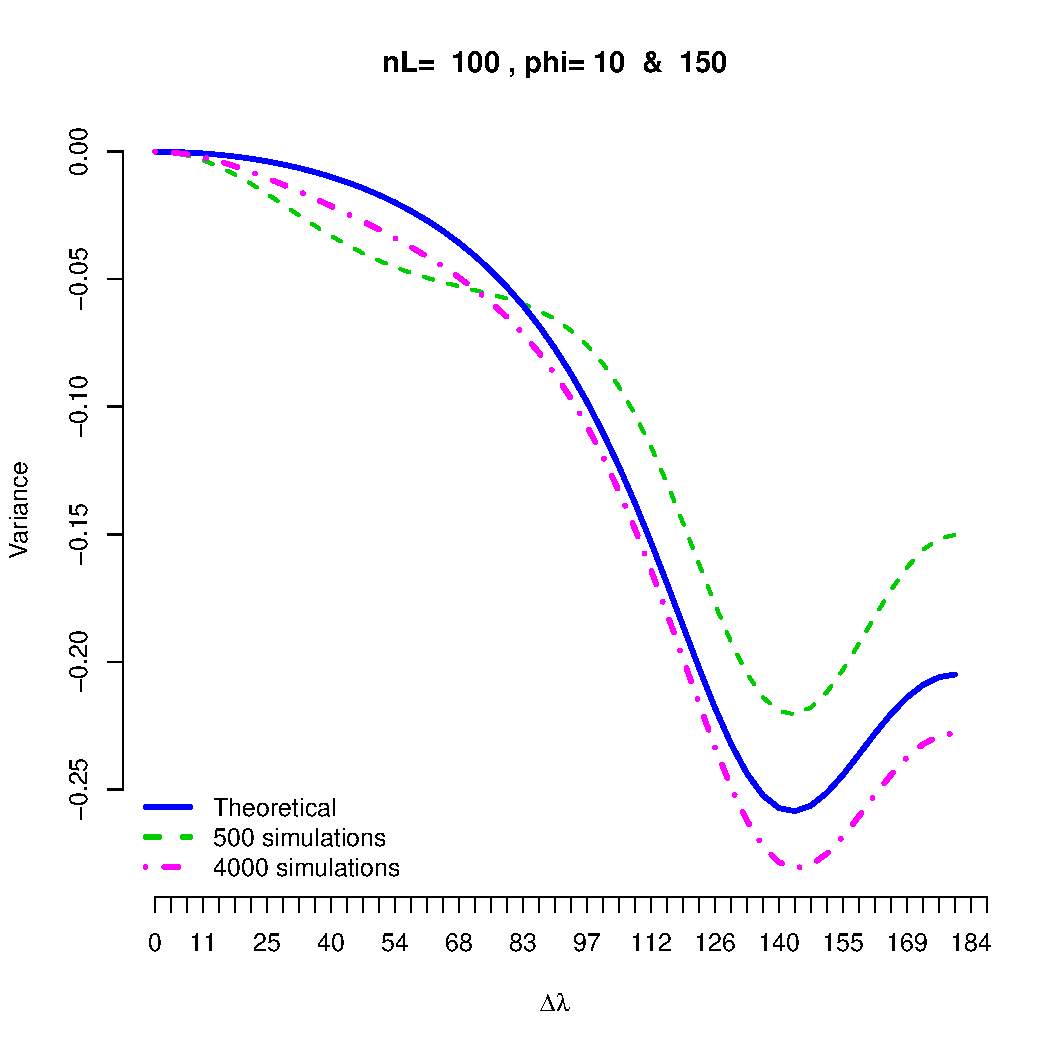
\includegraphics[width=1\linewidth]{graphs/results_variogram_model1_rpq}
		\caption{Using paramter Set 1 and $R(P,Q)$}
		\label{fig:sfig1}
	\end{subfigure}
	\begin{subfigure}{.5\textwidth}
		\centering
		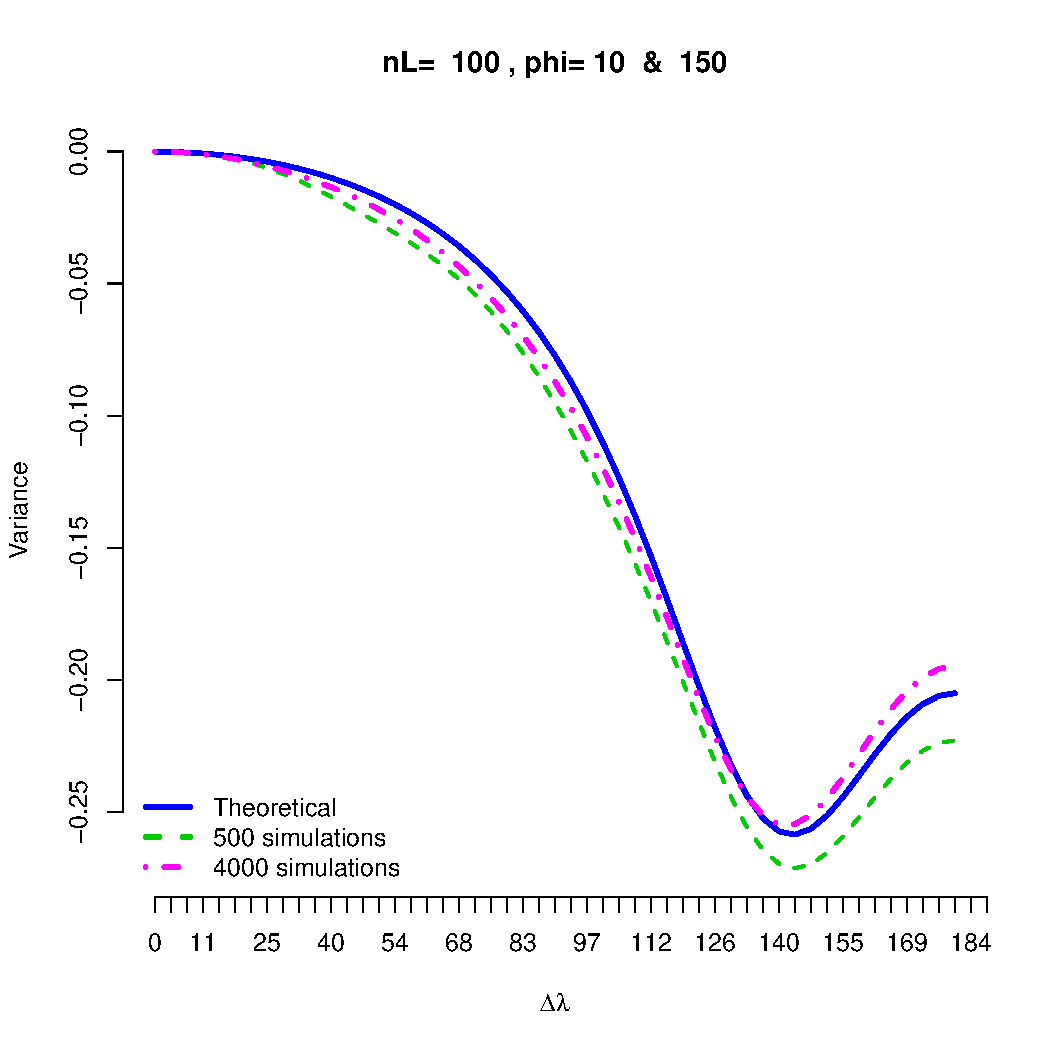
\includegraphics[width=1\linewidth]{graphs/results_variogram_model1}
		\caption{Using paramter Set 1 and $C_m$}
		\label{fig:sfig2}
	\end{subfigure}
	\begin{subfigure}{.5\textwidth}
		\centering
		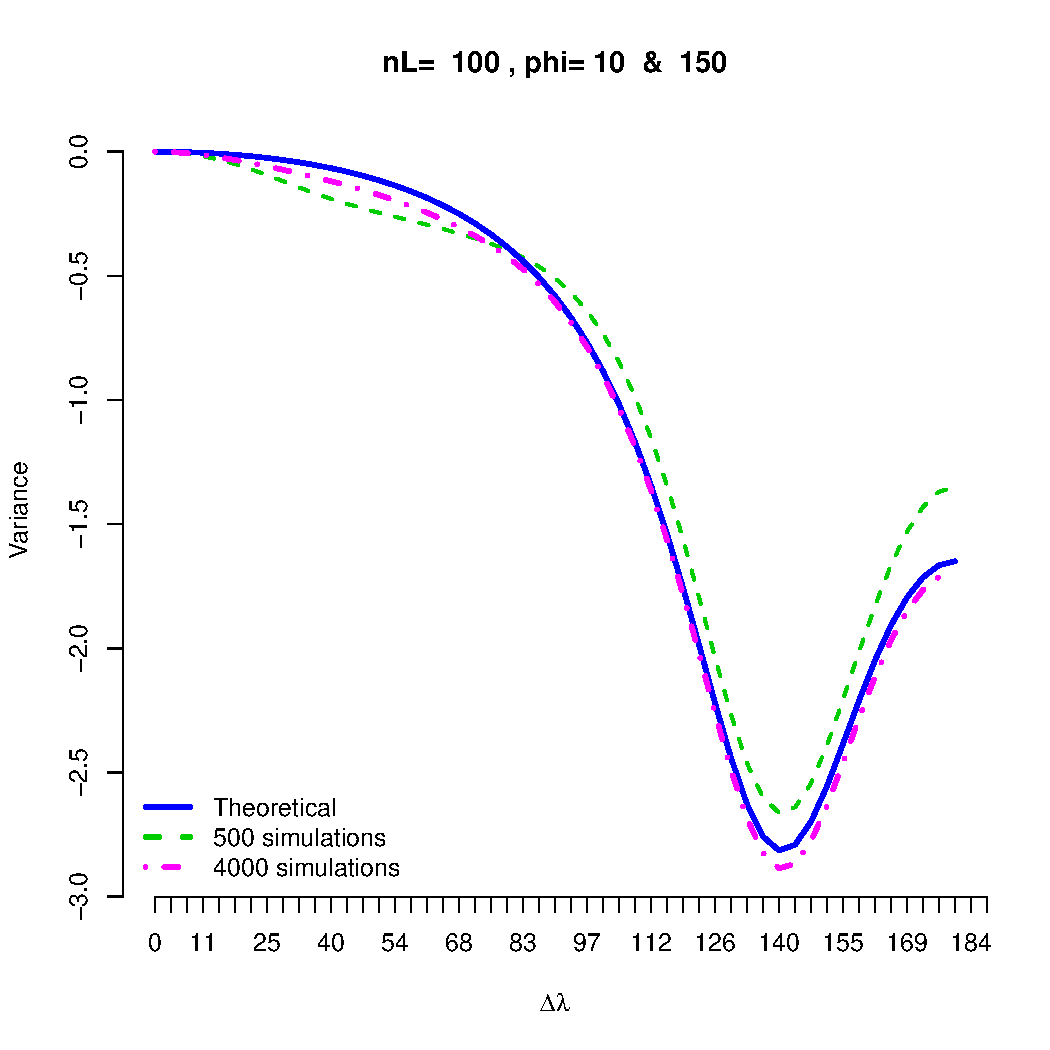
\includegraphics[width=1\linewidth]{graphs/results_variogram_model1_rpq_2}
		\caption{Using paramter Set 2 and $R(P,Q)$}
		\label{fig:sfig1}
	\end{subfigure}
	\begin{subfigure}{.5\textwidth}
		\centering
		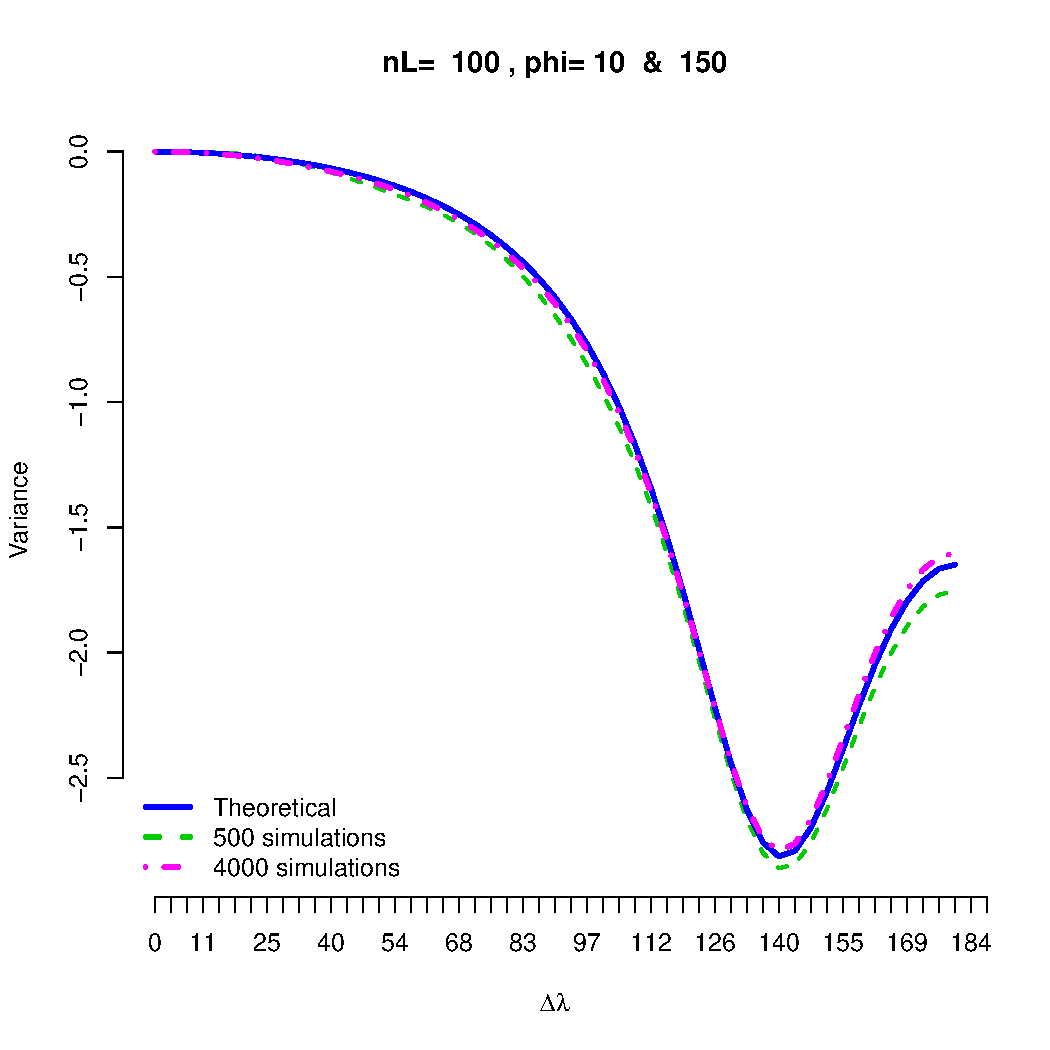
\includegraphics[width=1\linewidth]{graphs/results_variogram_model1_2}
		\caption{Using paramter Set 2 and $C_m$}
		\label{fig:sfig2}
	\end{subfigure}
	\caption[Using Parameter Set 1 and Set 2 to Perform The Variogram Estimator]{Using parameter Set 1 and Set 2 to perform the variogram estimator under model 1, solid line (blue) represents the theoretical values of cross variogram and dashed lines (green, purple) represents the estimates for 500 and 4000 simulations respectively. }
	\label{compare_varigram_sim_1}
\end{figure}


%-------------------------------------%
\subsection{Results for Longitudinally Reversible Processes}
%-------------------------------------%

Setting parameter $u = 0$ in all of our models yields longitudinally reversible covariance functions (see Figure \ref{fig_parameter_comp} 1(d) ). Based on 500 simulations, one can see that the cross variogram estimates from direct $R(P,Q)$ approach are slightly away from the theoretical values all three models (Figure \ref{logitudinal_comparison_rpq}). In contrast from the $C_m$ approach the estimates are very close to theoretical values (Figure \ref{logitudinal_comparison_cm}).

\begin{figure}[H]
	\centering
	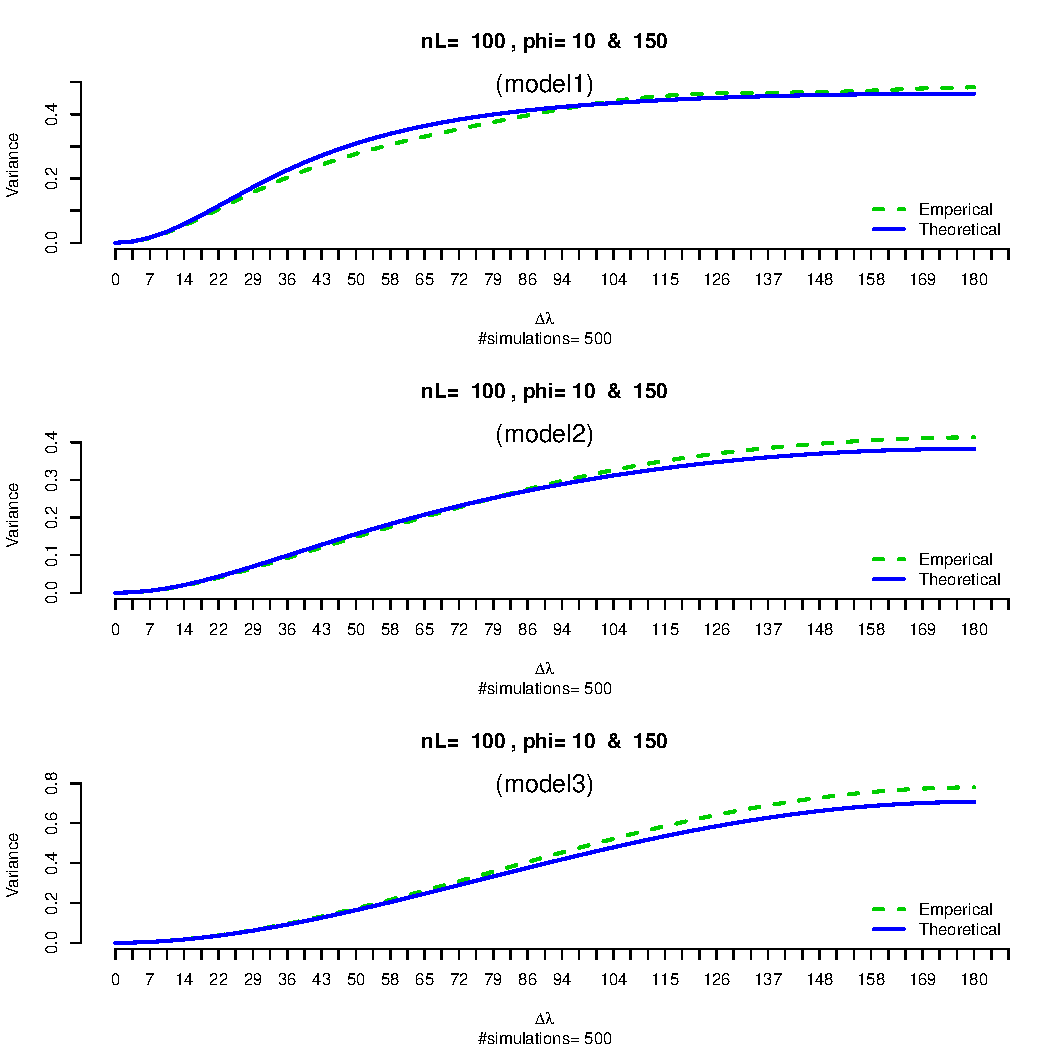
\includegraphics [scale =.9, keepaspectratio]{graphs/results_variogram_comparison_rpq}
	\caption[Based on $R(P,Q)$ Approach the Cross Variogram Estimator Comparison]{Based on $R(P,Q)$ approach the cross variogram estimator comparison for longitudinally reversible process using  model 1, model 2, and model 3 (when $u=0$).}
	\label{logitudinal_comparison_rpq}
\end{figure}

\begin{figure}[H]
	\centering
	% 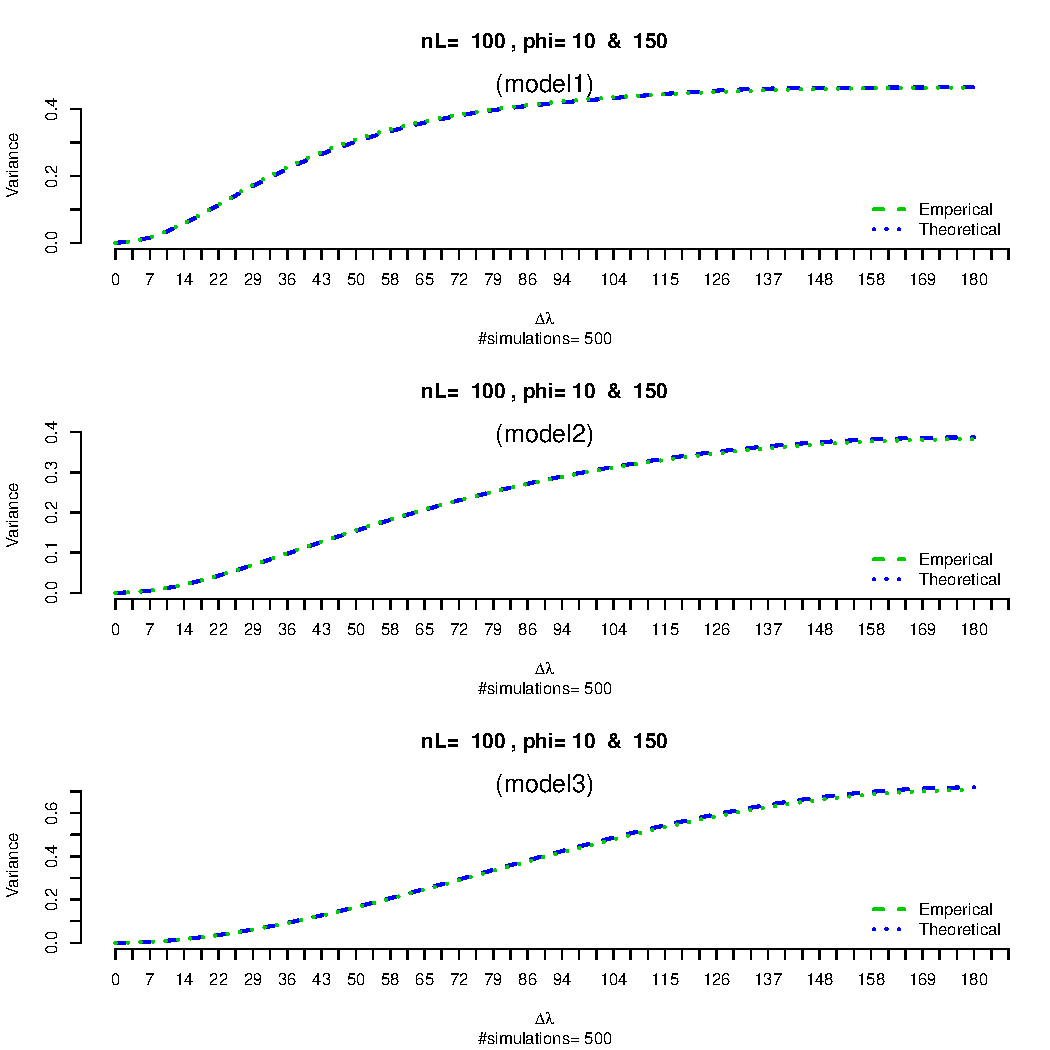
\includegraphics [width=0.9\textwidth ]{graphs/results_variogram_comparison}
	\includegraphics [scale =.9, keepaspectratio]{graphs/results_variogram_comparison_cm}
	% width=12cm,height=12cm
	\caption[Based on $C_m$ Approach the Cross Variogram Estimator Comparison]{Based on $C_m$ approach the cross variogram estimator comparison for longitudinally reversible process using  model 1, model 2, and model 3 (when $u=0$).}
	\label{logitudinal_comparison_cm}
\end{figure}


%-------------------------------------%
\subsection{Comparison of Cross Covariance}
%-------------------------------------%

As indicated from Chapter 4, when $C_0(\phi_P, \phi_Q) = 0$, the cross covariance MOM estimator is unbiased. Therefore we obtain the cross covariance MOM estimates given by \eqref{cross_covariance} under model 2 and model 3, and then compare them with the true values. Here we select two pairs of latitudes, $\phi = 70, 80$ ($20^0S$ ,$10^0S$) and $\phi = 60, 120$ ($30^0S$, $40^0N$). One can note that the cross covariance estimates match with the theoretical values very well (Figure \ref{cross_cov_comparison}).

%% individual cross covaraiance graphs
% \begin{figure}[H]
% \begin{center}
% 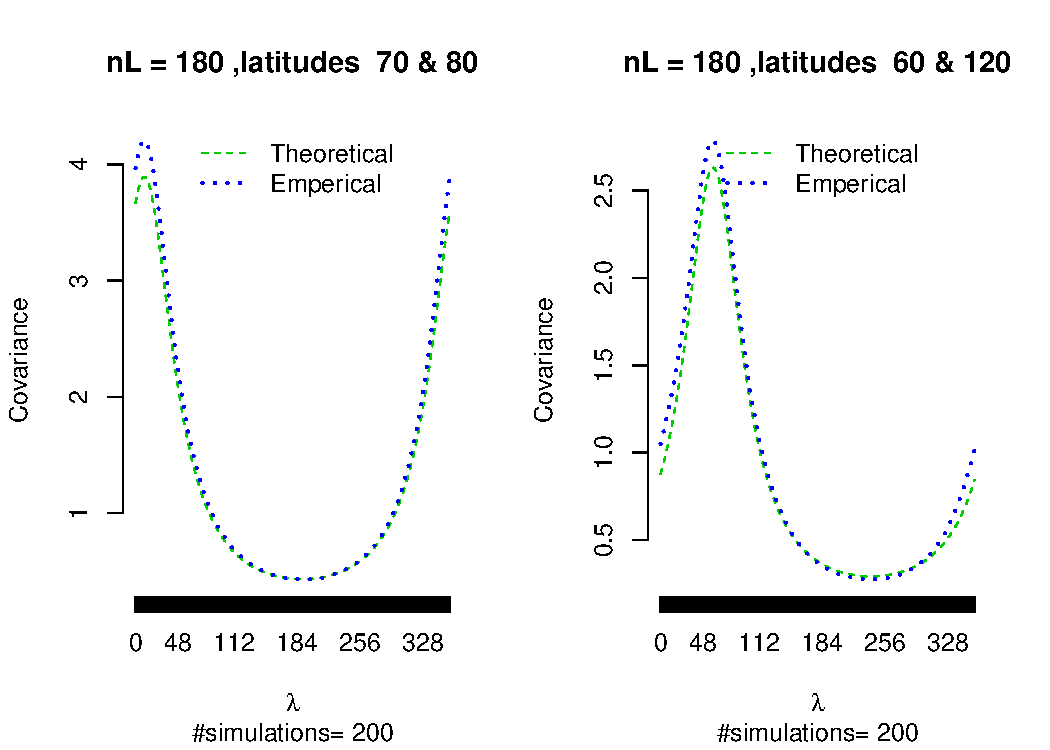
\includegraphics [width=0.75\textwidth ]{graphs/Model1.pdf}
% \caption{Cross covariance comparison of model1}
% \end{center}
% \end{figure}

% \begin{figure}[H]
% 	\begin{center}
% 		\includegraphics [width=0.75\textwidth ]{graphs/Model2.pdf}
% 		%\includegraphics [width=6in, height=3in]{Model2.pdf}
% 		\caption{Cross covariance comparison of model 2}
% 	\end{center}
% \end{figure}
% 
% 
% \begin{figure}[H]
% 	\begin{center}
% 		%\includegraphics [scale=.6]{Model3.pdf}
% 		\includegraphics [width=0.75\textwidth ]{graphs/Model3.pdf}
% 		\caption{Cross covariance comparison of model 3}
% 	\end{center}
% \end{figure}

\begin{figure}
	\begin{subfigure}{1\textwidth}
		\centering
		\includegraphics[keepaspectratio, scale=0.6]{graphs/Model2}
		\caption{Model 2 \eqref{model2}}
		\label{fig:cov2}
	\end{subfigure}
	\begin{subfigure}{1\textwidth}
		\centering
		\includegraphics[keepaspectratio, scale=0.6]{graphs/Model3}
		% \includegraphics[width=1\linewidth]{graphs/Model3}
		\caption{Model 3 \eqref{model3}}
		\label{fig:cov3}
	\end{subfigure}
\caption[Cross Covariance Comparison of Model 2 and Model 3]{Cross covariance comparison of model 2 and model 3}
\label{cross_cov_comparison}
\end{figure}


%-------------------------------------%
\subsection{Comparison of MSE}
%-------------------------------------%

In addition to comparing the biases, we also consider the mean square error (MSE) of the MOM cross variogram estimates obtained under both $C_m$ and direct $R(P,Q)$ approaches. The overall MSE is calculated based on the following formula.
\begin{eqnarray*}
MSE &=& \frac{1}{n_L} \sum (var + bias^2) \\
    &= & \frac{1}{n_L} \sum_{j=1}^{n_L} \left[ \frac{1}{nn}\sum_{i=1}^{nn}\left(\hat{\gamma_{i}}(j\delta)-\overline{\hat{\gamma}(j\delta)})^2\right) +  (\gamma_(j\delta) - \overline{\hat{\gamma}(j\delta)})^2 \right]
\end{eqnarray*}

\noi where $\delta = \frac{2\pi}{n_L}$ and $nn$ is the number of simulations.

\begin{figure}[H]
	\begin{subfigure}{.5\textwidth}
		\centering
		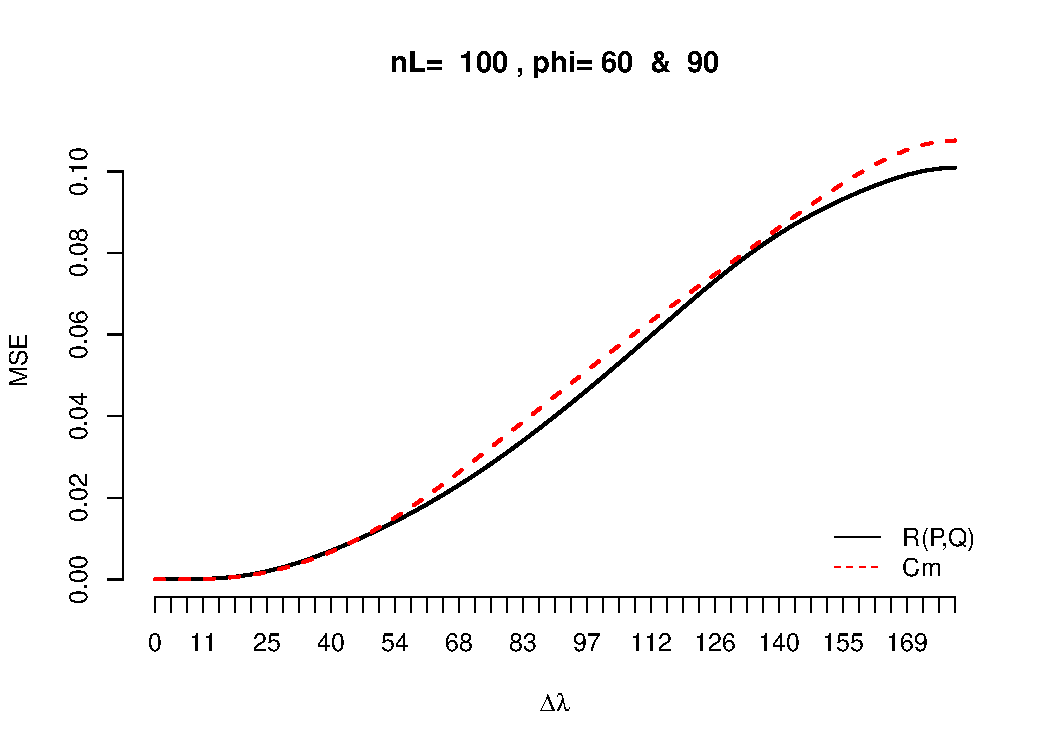
\includegraphics[width=1\linewidth]{graphs/MSE_comparison_model1_60_90}
		\caption{Model 1 (pair 1)}
		\label{fig:mse1}
	\end{subfigure}
	\begin{subfigure}{.5\textwidth}
		\centering
		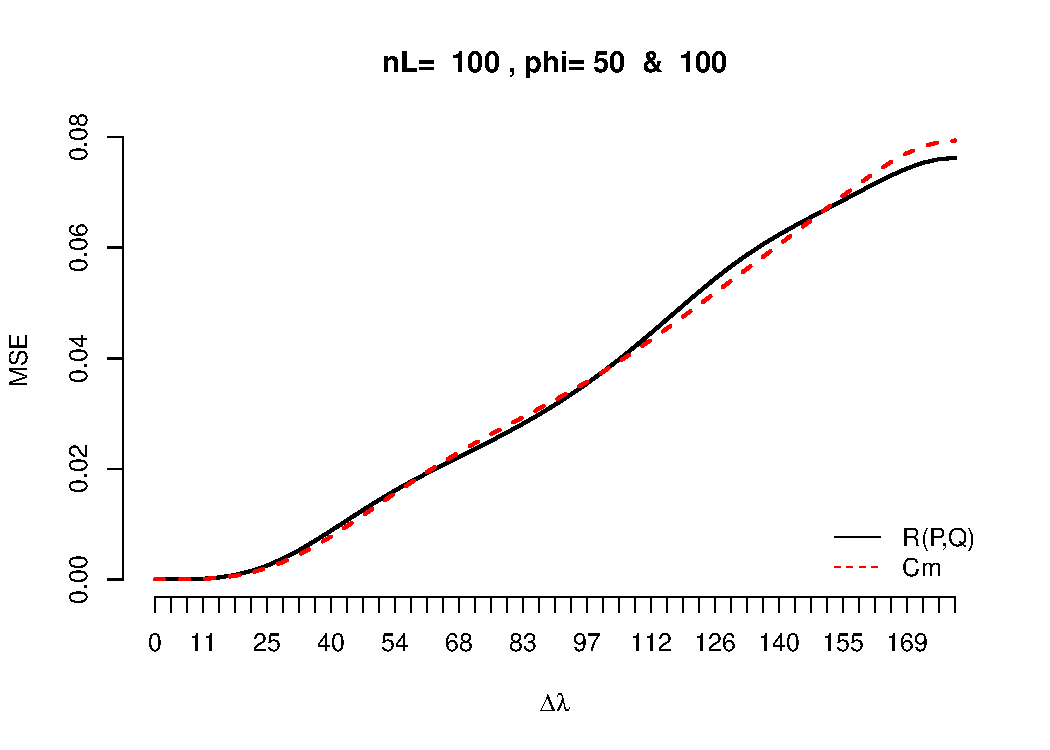
\includegraphics[width=1\linewidth]{graphs/MSE_comparison_model1_50_100}
		\caption{Model 1 (pair 2)}
		\label{fig:mse2}
	\end{subfigure}
		\begin{subfigure}{.5\textwidth}
		\centering
		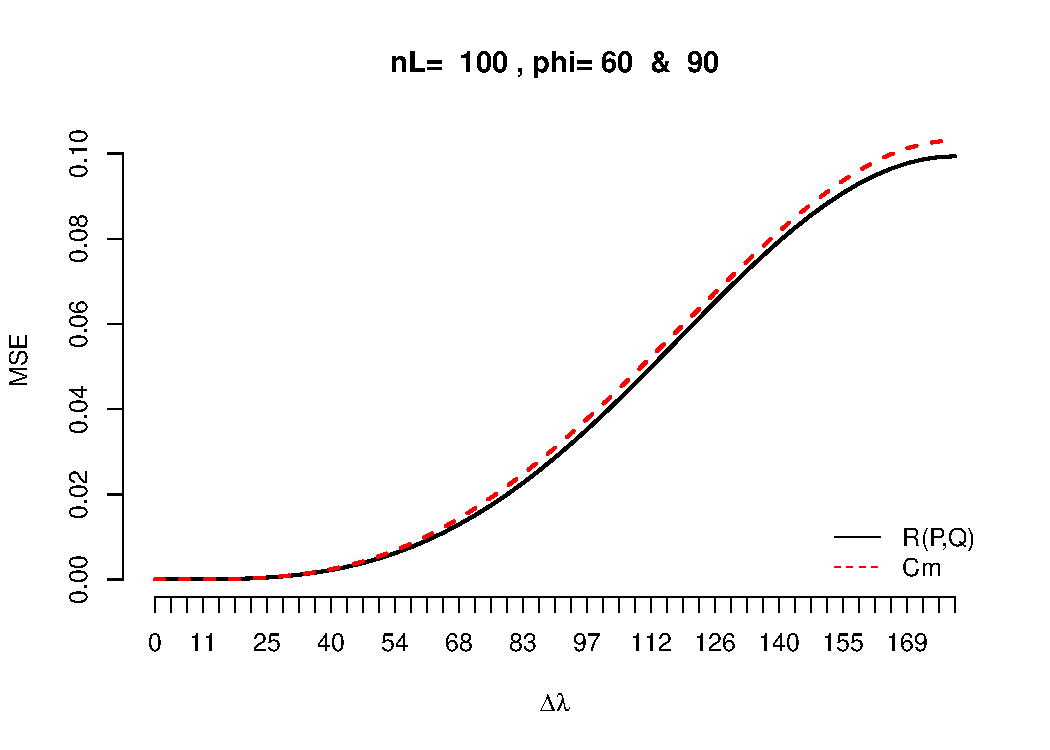
\includegraphics[width=1\linewidth]{graphs/MSE_comparison_model2_60_90}
		\caption{Model 2 (pair 1)}
		\label{fig:mse3}
	\end{subfigure}
		\begin{subfigure}{.5\textwidth}
		\centering
		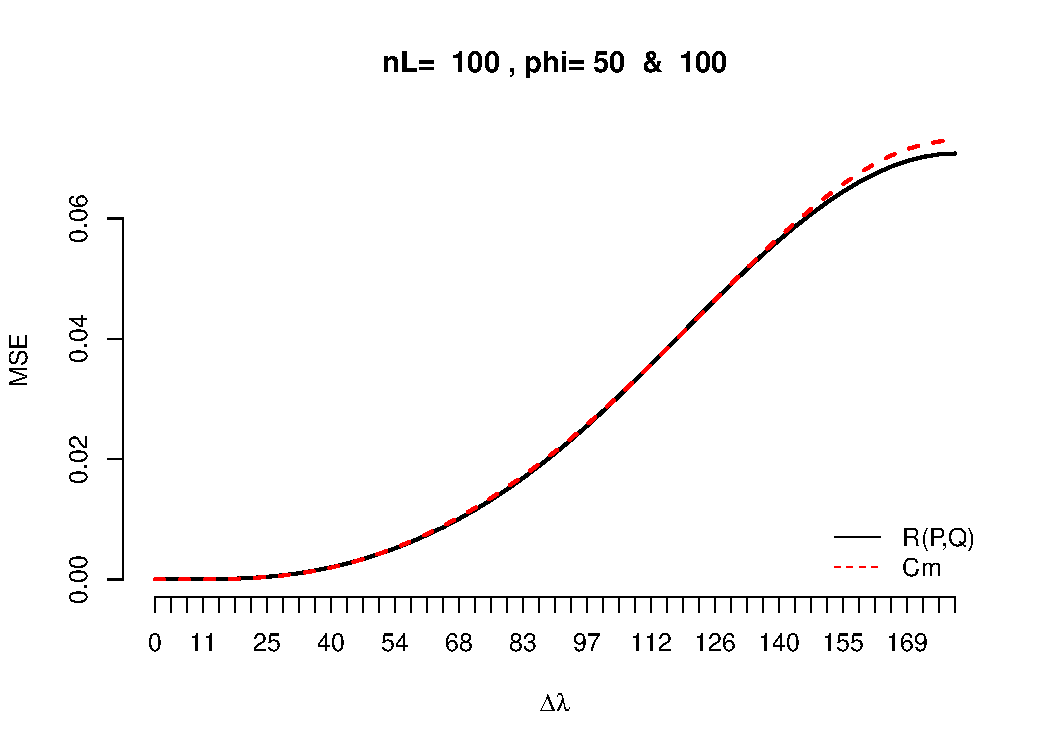
\includegraphics[width=1\linewidth]{graphs/MSE_comparison_model2_50_100}
		\caption{Model 2 (pair 2) }
		\label{fig:mes4}
	\end{subfigure}
	\caption[MSE Comparison Between $C_m$ and $R(P,Q)$ Using 500 Simulations]{MSE comparison between $C_m$ and $R(P,Q)$ using 500 simulations; pair 1 ($30^0S,0^0$), pair 2 ($40^0S, 10^0N$) figures (a) - (b) is the comparison for model 1 and figure (c)-(d) is the comparison for model 2 }
	\label{mse_comparison}
\end{figure}

\begin{table}[H]
\label{parameters}
\centering
\caption[MSE Comparison for $C_m$ and $R(P,Q)$ Approaches, the Values in Paranthesis]{MSE comparison for $C_m$ and $R(P,Q)$ approaches, the values in paranthesis are the bias for each pair.  Set 1 and Set 2 are referring to the set of parameters discussed in simulation setup}
\vskip 16pt
\begin{tabular}{|l|c|l|l|l|l|}
\hline
\multicolumn{2}{|c|}{}      & \multicolumn{2}{|c|}{Set 1} & \multicolumn{2}{|c|}{Set 2}  \\ \hline
Model & $(\phi_P, \phi_Q)$  & $R(P,Q)$  & $C_m$           & $R(P,Q)$  & $C_m$  \\ \hline
\multirow{6}{*}{Model1} & \multirow{2}{*}{(60, 90)}  & 2.298    & 2.427	  & 15.688	& 16.384	 \\
                        & &                            (0.0022) & (0.0004)& (0.0250)& (0.0015)	\\ \cline{2-6}
                        & \multirow{2}{*}{(50, 100)} & 1.784    & 1.782	  & 13.295 	& 12.767 	 \\
                        & &                            (0.0009) &(0.0001) & (0.0193)& (0.0030) 	 \\ \cline{2-6}
                        & \multirow{2}{*}{(10, 150)} & 0.564    & 0.623	  & 8.062	  & 9.177	 \\ 
                        & &                            (0.0009) &(0.0001) & (0.0226)& (0.0023)	 \\ \hline
\multirow{6}{*}{Model2} & \multirow{2}{*}{(60, 90)}  & 2.000    & 2.080	  & 12.452	& 13.021	 \\
                        & &                            (0.0004) & (0.0004)& (0.0042) & (0.0023)	\\ \cline{2-6}
                        & \multirow{2}{*}{(50, 100)} & 1.437    & 1.459	  & 9.196	  & 9.262 	 \\
                        & &                            (0.0001) &(0.0000) & (0.0015)& (0.0006) 	 \\ \cline{2-6}
                        & \multirow{2}{*}{(10, 150)} & 0.457    & 0.512	  & 6.034	  & 7.266	 \\ 
                        & &                            (0.0014) &(0.0001) & (0.0337)& (0.0026)	 \\ \hline
\end{tabular}
\end{table}

One can see from the above table that a variety of pairs of latitudes and two different sets of parameters are used in simulations. The MSEs from $C_m$ are comparable with those from direct $R(P,Q)$ approach while the $C_m$ approach gives smaller bias.



%
% \[
% MSE = \frac{1}{n_L-1}\sum_{k=1}^{n_L} (\gamma_{k}(\Delta\lambda) - \overline{\hat{\gamma}_{k}(\Delta\lambda)})^2
% \]

% \begin{table}[H]
% \label{parameters}
% \centering
% \begin{tabular}{|l|l|l|l|l|l|l|}
% \hline
%  & \multicolumn{2}{|c|}{Model 1} & \multicolumn{2}{|c|}{Model 2} & \multicolumn{2}{|c|}{Model 3} \\ \cline{2-7}
% Parameters & $R(P,Q)$  & $C_m$  & $R(P,Q)$  & $C_m$ & $R(P,Q)$  & $C_m$ \\ \hline
% % set 1 & 	0.04825 & 0.00881   & 	0.01820 & 0.00534 & 	-- & 0.01426 \\
% % set 2 & 	1.15598 & 0.16591   & 	0.42931 & 0.14270 & 	-- & 0.33726 \\ \hline \hline
%
% set 1 & 0.000965 &  0.0001762	& 0.000364	& 0.000107	&--&	0.0002852 \\
% set 2 & 0.023119 &  0.0033182	& 0.0085862	& 0.002854	&--&	0.0067452 \\ \hline \hline
%
% %model 1 4000 Cm 0.03085625
% %model 1 4000 R(P,Q) 0.1144611
%
% \end{tabular}
% \caption{MSE comparison}
% \end{table}

% Now the MSE for $R(P,Q)$ is lower but the bias is higer (bias for $C_m = 0.0325219$ and $R(P,Q) = 0.2493109$.)


%-------------------------------------%
\subsection{Generated Data}
%-------------------------------------%

\begin{figure}[H]
	\centering
		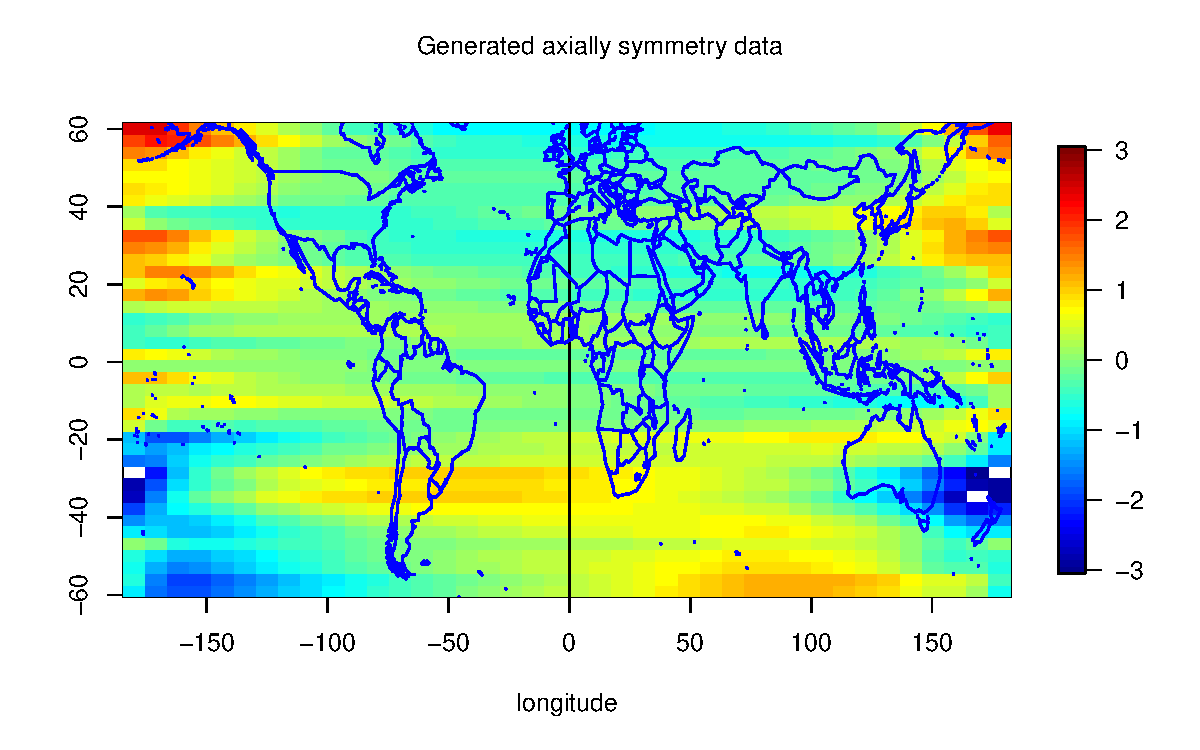
\includegraphics [width=1\textwidth ]{graphs/Data_sample_120_model2_withmap.pdf}
		\caption[A Snapshot of Global Data Generated Based on $C_m$ Approach using Zero]{A snapshot of global data generated based on $C_m$ approach using zero mean random process (model 2)}
		\label{grid_plot_model_2}
\end{figure}
The Figure \ref{grid_plot_model_2} is a snapshot of the global data generated based on model 2 and could potentially be used later for research. Clearly there are spatial trends within the latitudes but not within longitudes. It is somewhat difficult to use the covariance structure to generate data when it is closer to Earth's pole (similar complexity can also be observed in MSU and TOMS data). Therefore we produced a snapshot by generating the data on $[0,2\pi/3] \times [0,2\pi]$ (equivalent to $[-\pi/3,\pi/3] \times [-\pi,\pi]$ ) grid, with a grid resolution of $1^0\times 2^0$ ({\em i.e } $n_l = 120, n_L=180 \Rightarrow$ 21600 spatial points). However we observed some inconsistencies (strong spots) when examining closer close to the boundary points of longitudes ($\lambda \rightarrow \pm \pi$).

\begin{figure}[H]
	\begin{center}
		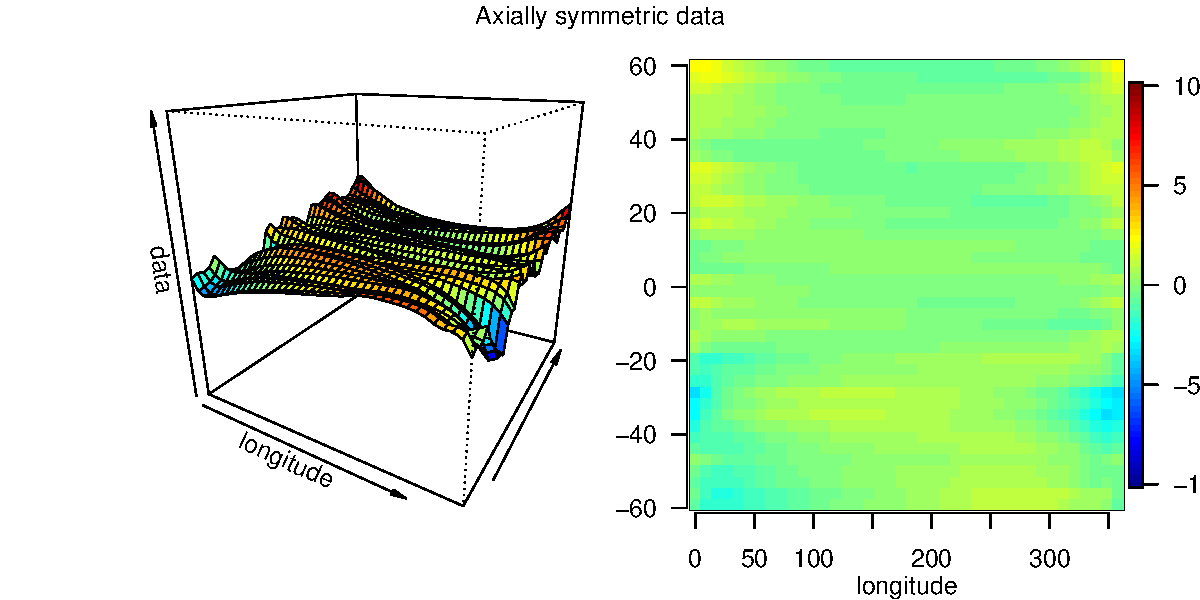
\includegraphics [width=0.9\textwidth ]{graphs/Data_sample_120_model2_density.pdf}
		\caption[One Snapshot of The Axially Symmetric Data Generated Based on Model 2]{One snapshot of the axially symmetric data generated based on model 2, grid resolution $2^0\times 1^0$ (data scale -10 and 10).}
			\label{grid_plot_model2_sim2}
	\end{center}
\end{figure}
The above Figure \ref{grid_plot_model2_sim2} refers to the data snapshot given by Figure \eqref{grid_plot_model_2} and it is clear that trends are within latitudes not within longitudes. Four snapshots of the gridded data generated based on all models are given in Appendix \ref{appendixA}.

%\end{document}


%------------------------------------%
\section{Discussion}
%------------------------------------%
The data generation algorithm proposed in this dissertation seems producing axially symmetric data that follow the given covariance models. The bias of the cross variogram estimates from the data generated based on our algorithm is generally smaller than that from direct $R(P,Q)$ approach, while maintaining the same level of MSEs. The computation cost for our algorithm is very small, with the order of $O(n_L n_l^2)$. This is much smaller than that when taking the square root of $R(P,Q)$ through SVD decomposition. Note that the dimension of $R(P,Q)$ is $n_ln_L \times n_ln_L$, which might be expensive or even not possible when performing the SVD with large dimension. In addition, obtaining $R(P,Q)^{1/2}$ with the light of block circulant matrix seems unclear. \cite{Li2013} indicated that one might find the eigenvalues using the properties of block circulant matrices, more specifically, they pointed out these eigenvalues are related to sub-matrices $R_0, R_1, \ldots, R_{n_L-1}$. However, since these matrices are not necessary symmetric, their eigenvalues could be complex-valued or negative. When submatrices are symmetric, \cite{Tee2005} proposed some methods to find the eigenvalues. This will be extensively explored in the future.



%%------------------------------------------------------------------%%
\chapter{Future Research}
%\documentclass[12pt, amstex, letterpaper] {report} %{article}


\usepackage[margin=1in]{geometry}
\topmargin -0.5in \textwidth 6.5in \textheight 9in
\footskip .5in
\headheight 0.3in


\usepackage{Sweave}

\DefineVerbatimEnvironment{Sinput}{Verbatim} {xleftmargin=0em,frame=single}
\DefineVerbatimEnvironment{Soutput}{Verbatim} {xleftmargin=0em,frame=single}

\usepackage{amssymb, mathrsfs, amsmath, amsfonts}
\usepackage{enumerate, comment}
\usepackage{hyperref, natbib,apalike, float} %cite
\usepackage{color, multirow, setspace, fancyhdr,graphicx}
\usepackage{undertilde}
\usepackage[bottom]{footmisc}
\usepackage{graphicx}
\usepackage{framed}
\usepackage{subcaption}
\usepackage{amsthm}

%\doublespacing
\pagestyle{empty}
\pagestyle{fancy}
\lhead{ }
%\rhead{May 2016}
\fancyfoot{ }
\rfoot{Dissertation $|$ \thepage}
\lfoot{Chris Vanlangenberg}
\date{}

\includecomment{comment}

\newtheorem{theorem}{Theorem}[section]
\newtheorem{defn}{Definition}[section]
\newtheorem{prop}{Proposition}
\newcommand{\pro}[1]{\begin{prop}{#1}\end{prop}}

%\newtheorem{proof}{proof}
\newtheorem{rmk}{Remark}
\newcommand{\rmark}[1]{\begin{rmk}{#1}\end{rmk}}

\numberwithin{equation}{section}
\renewcommand{\footrulewidth}{0.1pt}
\renewcommand{\headrulewidth}{0.1pt}


\newcommand{\eqn}[1]{\begin{equation}{#1}\end{equation}}

\newcommand{\beq}{\begin{equation}}
\newcommand{\eeq}{\end{equation}}
%\renewcommand\refname{Literature}
\newcommand{\blue}[1]{\textcolor{blue}{\emph{#1}}}
\newcommand{\red}[1]{\textcolor{red}{\emph{#1}}}
\newcommand{\twoc}[2]{{\textcolor{blue}{#1}} and {\textcolor{red}{#2}}}


\newcommand{\xn}{x_1,\ldots, x_n}
\newcommand{\Xn}{X_1,\ldots, X_n}
\newcommand\floor[1]{\lfloor{#1}\rfloor}
\newcommand\ceil[1]{\lceil{#1}\rceil}

\newcommand{\X}{\mathcal{X}}
\newcommand{\Sp}{\mathbb{S}}
\newcommand{\R}{\mathbb{R}}
\newcommand{\C}{\mathbb{C}}
\newcommand{\pd}{positive definite }



\newcommand{\code}[1]{{\small\texttt{#1}}}
\newcommand{\pkg}[1]{{\normalfont\textsf{#1}}}
\newcommand{\var}[1] {{\normalfont\textbf{#1}}}
\newcommand{\Cm}{$C_m(\phi_P, \phi_Q)\ $}

\newcommand{\jun}{\cite{JunStein2008}}
%\begin{document}

In this dissertation research, we focus on data generation and estimation for axially symmetric processes on the sphere. We first show that for the stationary random process on the circle, the commonly used covariance function estimator based on Method of Moments (MOM) is biased with non-estimable bias, while the unbiased MOM variogram estimator is inconsistent. Our second project emphasizes on data generation, in which the axially symmetric random process can be decomposed as Fourier series on circles, where the Fourier random coefficients can be expressed as circularly-symmetric complex random vectors. We develop an algorithm that generates axially symmetric data with the given covariance model. All of the above results and theories have been supplemented via simulations. 

We can extend this dissertation work to a number of future research areas. We will first explore the unbiasedness and consistency of the MOM covariance and variogram estimators for homogeneous and axially symmetric random processes on the sphere. In particular, we expect a similar result holds for axially symmetric random processes. On the other hand, we will also explore the ergodic condition (if exists) that ensures the consistency of these estimators.

We have noticed that our proposed data generation algorithm assumes the closed form of $C_m(\phi_P, \phi_Q)$, which sometimes may not be available. This might restrict the applicability of our data generation algorithm. Note that in order to implement the algorithm, we only need the $C_m(\phi_P, \phi_Q)$ over the gridded locations. Therefore, given the covariance structure $R(P, Q)$, we may use the Discrete Fourier Transform to obtain those gridded $C_m(\phi_P, \phi_Q)$ values. This would definitely complement our dissertation research.

Kriging, or making predictions at unobserved locations, has always been one of the important applications of data modeling and analysis in spatial statistics. With the complexity and dimensionality of global data, it is highly demanded that practically useful parametric models with interpretable parameters would be available for geography and environmental scientists. As the continuation of this dissertation research, we wish to enhance the kriging techniques and make use of proposed global data generation methods to make global predictions with less dimensionality.

%\end{document}

%%------------------------------------------------------------------%%
%%------------------------ Bibliography ----------------------------%%
%%------------------------------------------------------------------%%
%% Replace the myreferences with the name of your bib file.  Then you
%% can run bibtex as usual.  See tips for details.
%%------------------------------------------------------------------%%

\bibliography{biblography}
\bibliographystyle{amsalpha}

%%------------------------------------------------------------------%%
%%------------------------- Appendices -----------------------------%%
%%------------------------------------------------------------------%%
%% If you choose not to have appendices, comment out the \appendix
%% line and the chapters below.
%%------------------------------------------------------------------%%
\appendix
\chapter{Data snapshots for all Models}  \label{appendixA}
%\section*{\centering Appendix A }
%%%%%%%% this is a appendix for simulation results
% \documentclass[12pt, amstex, letterpaper] {report} %{article}


\usepackage[margin=1in]{geometry}
\topmargin -0.5in \textwidth 6.5in \textheight 9in
\footskip .5in
\headheight 0.3in


\usepackage{Sweave}

\DefineVerbatimEnvironment{Sinput}{Verbatim} {xleftmargin=0em,frame=single}
\DefineVerbatimEnvironment{Soutput}{Verbatim} {xleftmargin=0em,frame=single}

\usepackage{amssymb, mathrsfs, amsmath, amsfonts}
\usepackage{enumerate, comment}
\usepackage{hyperref, natbib,apalike, float} %cite
\usepackage{color, multirow, setspace, fancyhdr,graphicx}
\usepackage{undertilde}
\usepackage[bottom]{footmisc}
\usepackage{graphicx}
\usepackage{framed}
\usepackage{subcaption}
\usepackage{amsthm}

%\doublespacing
\pagestyle{empty}
\pagestyle{fancy}
\lhead{ }
%\rhead{May 2016}
\fancyfoot{ }
\rfoot{Dissertation $|$ \thepage}
\lfoot{Chris Vanlangenberg}
\date{}

\includecomment{comment}

\newtheorem{theorem}{Theorem}[section]
\newtheorem{defn}{Definition}[section]
\newtheorem{prop}{Proposition}
\newcommand{\pro}[1]{\begin{prop}{#1}\end{prop}}

%\newtheorem{proof}{proof}
\newtheorem{rmk}{Remark}
\newcommand{\rmark}[1]{\begin{rmk}{#1}\end{rmk}}

\numberwithin{equation}{section}
\renewcommand{\footrulewidth}{0.1pt}
\renewcommand{\headrulewidth}{0.1pt}


\newcommand{\eqn}[1]{\begin{equation}{#1}\end{equation}}

\newcommand{\beq}{\begin{equation}}
\newcommand{\eeq}{\end{equation}}
%\renewcommand\refname{Literature}
\newcommand{\blue}[1]{\textcolor{blue}{\emph{#1}}}
\newcommand{\red}[1]{\textcolor{red}{\emph{#1}}}
\newcommand{\twoc}[2]{{\textcolor{blue}{#1}} and {\textcolor{red}{#2}}}


\newcommand{\xn}{x_1,\ldots, x_n}
\newcommand{\Xn}{X_1,\ldots, X_n}
\newcommand\floor[1]{\lfloor{#1}\rfloor}
\newcommand\ceil[1]{\lceil{#1}\rceil}

\newcommand{\X}{\mathcal{X}}
\newcommand{\Sp}{\mathbb{S}}
\newcommand{\R}{\mathbb{R}}
\newcommand{\C}{\mathbb{C}}
\newcommand{\pd}{positive definite }



\newcommand{\code}[1]{{\small\texttt{#1}}}
\newcommand{\pkg}[1]{{\normalfont\textsf{#1}}}
\newcommand{\var}[1] {{\normalfont\textbf{#1}}}
\newcommand{\Cm}{$C_m(\phi_P, \phi_Q)\ $}

\newcommand{\jun}{\cite{JunStein2008}}
% \begin{document}
% \section{Simulations}

\begin{figure}[H]
\label{grid_plot_model1}
\begin{center}
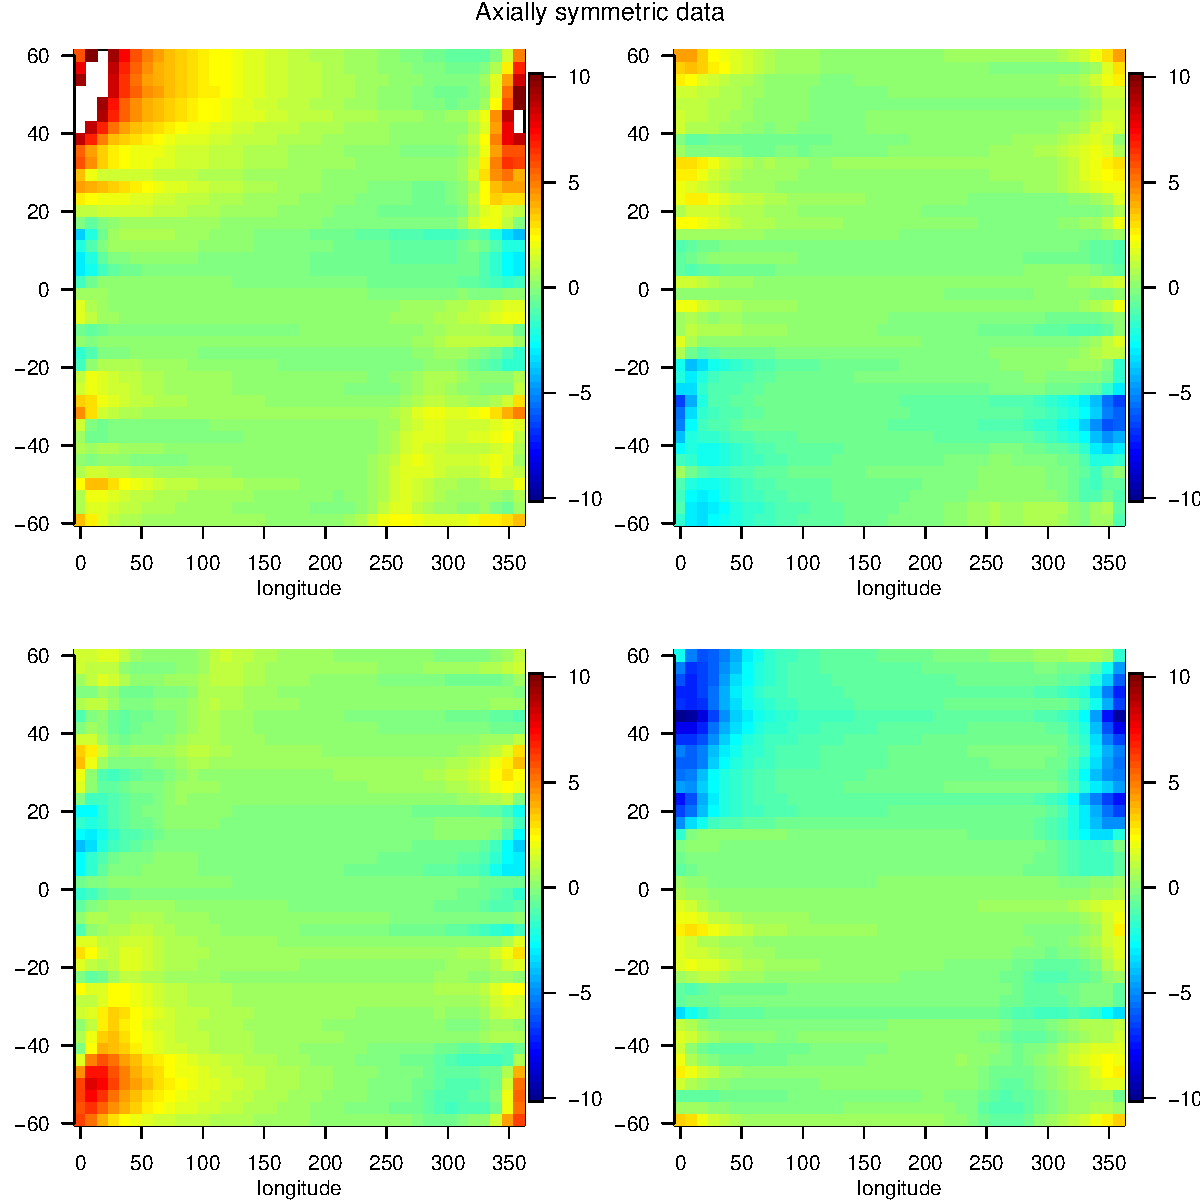
\includegraphics [scale=.8]{graphs/Data_sample_120_model1.pdf}
\caption*{Four consecutive axially symmetric data snapshots based on model 1, grid resolution $2^0\times 1^0$ (data scale -10 and 10).}
\end{center}
\end{figure}

\begin{figure}[H]
	\label{grid_plot_model2}
	\begin{center}
		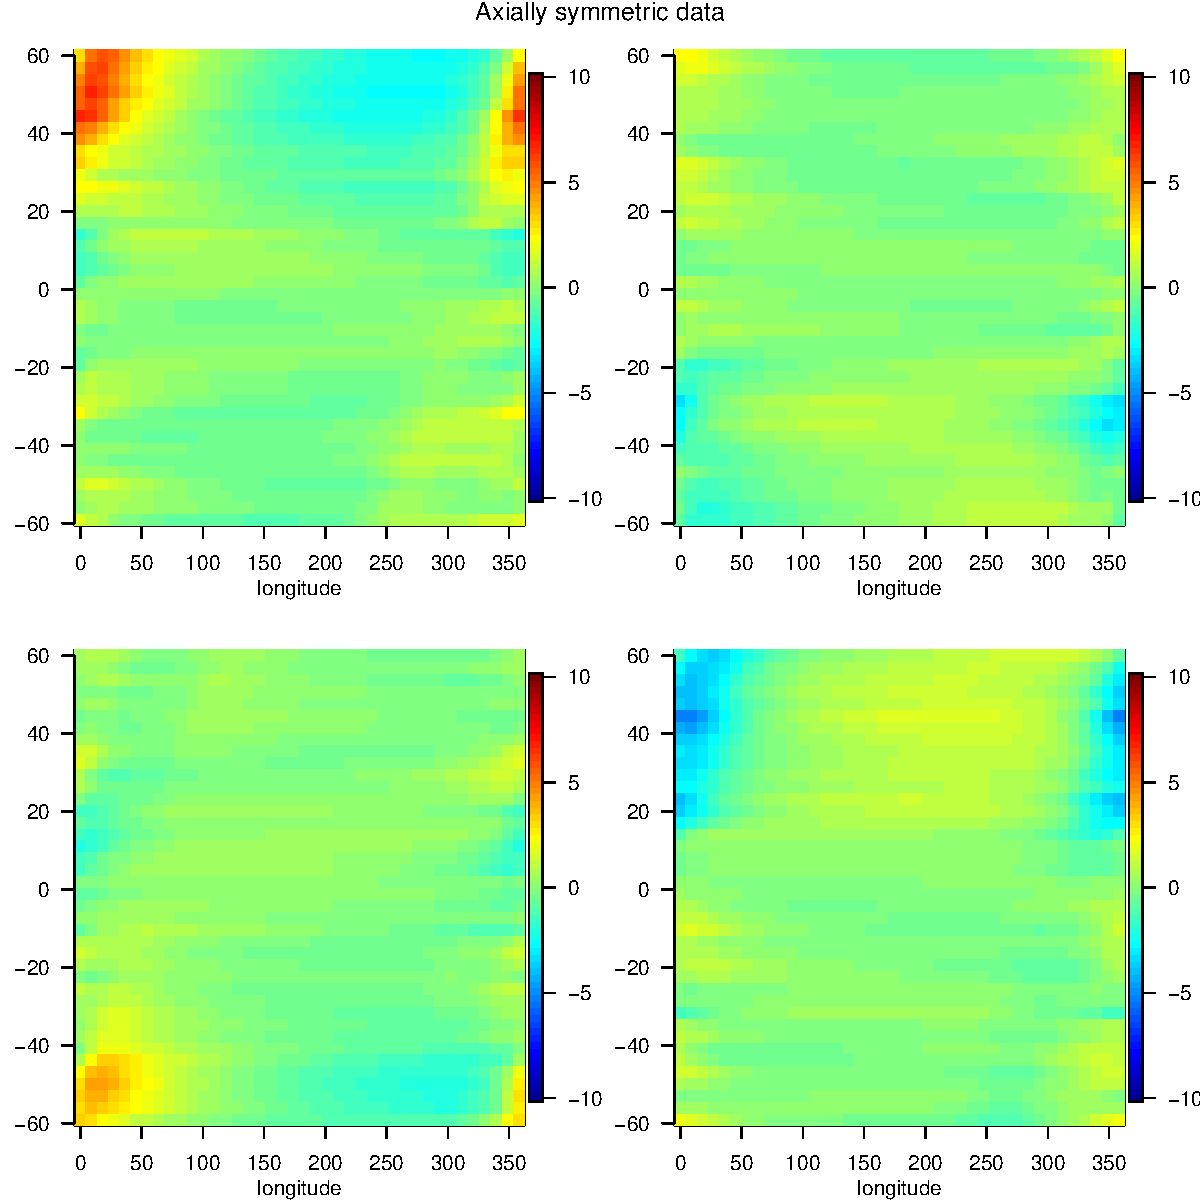
\includegraphics [scale=.8]{graphs/Data_sample_120_model2.pdf}
		\caption{Four consecutive axially symmetric data snapshots based on model 2, grid resolution $2^0\times 1^0$ (data scale -10 and 10).}
	\end{center}
\end{figure}


\begin{figure}[H]
\label{grid_plot_model3}
\begin{center}
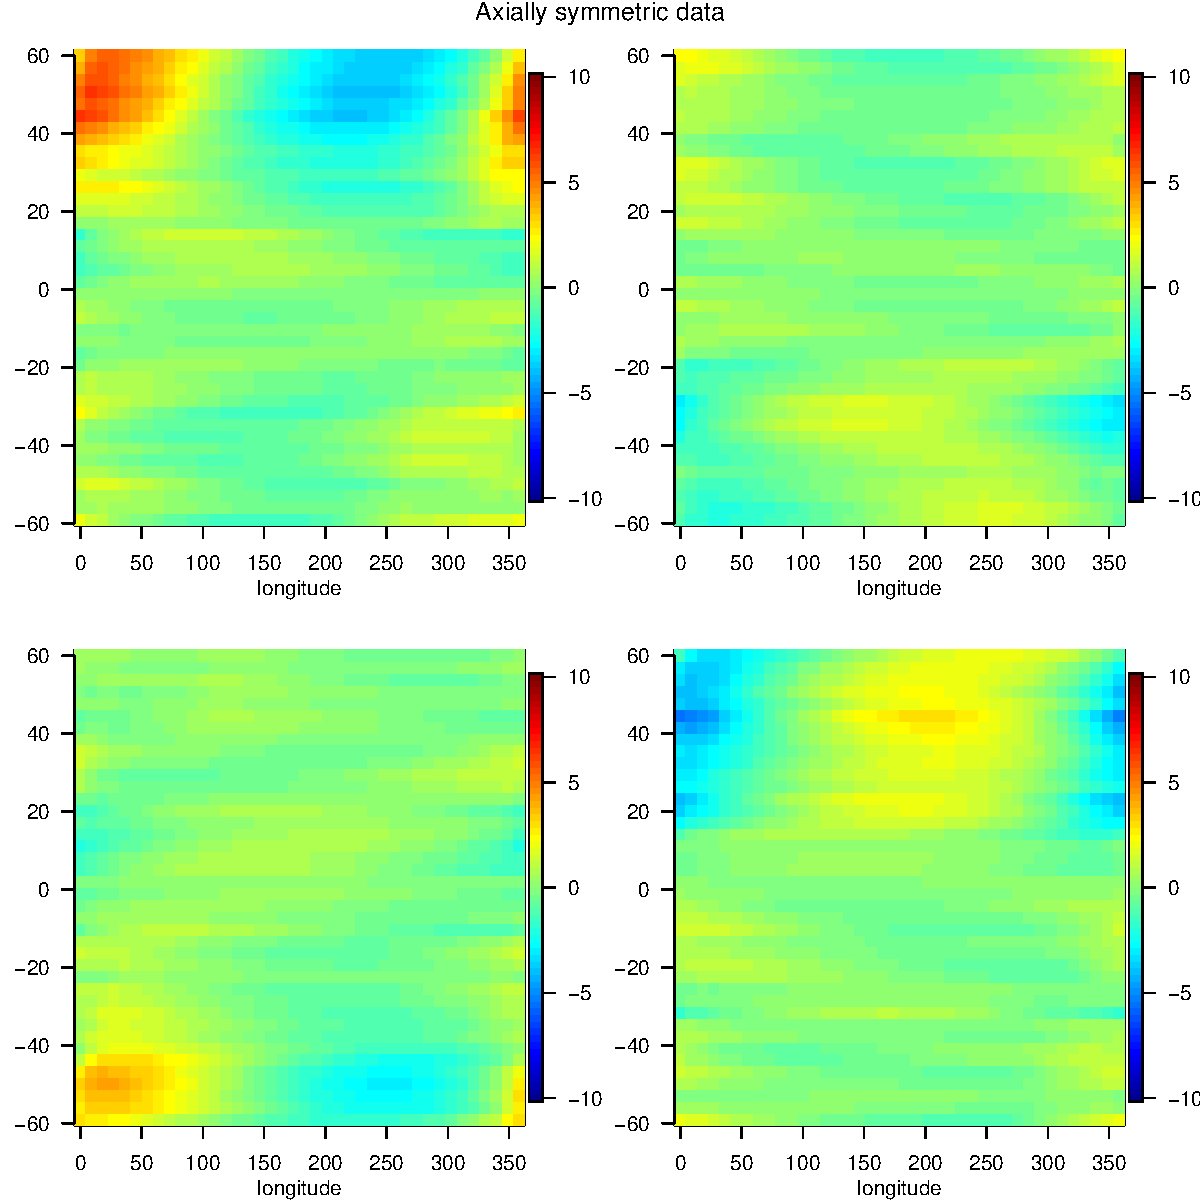
\includegraphics [scale=.8]{graphs/Data_sample_120_model3.pdf}
\caption*{Four consecutive axially symmetric data snapshots based on model 3, grid resolution $2^0\times 1^0$ (data scale -10 and 10).}
\end{center}
\end{figure}


%%------------------------------------------------------------------%%
\backmatter % required
%%------------------------------------------------------------------%%
%%----------------------- YOU ARE FINISHED ! -----------------------%%
%%------------------------------------------------------------------%%

\end{document}
